\chapter{Implementacja sprzętowo-programowa systemu wizyjnego}

%TODO krótki wstępn. M. in. po co implementacja sprzętowa.
Celem implementacji sprzętowej jest realizacja określonej funkcjonalności przez dany układ scalony. W przeciwieństwie do programu komputerowego, urządzenie realizujące sprzętowo odpowiednio zaimplementowany algorytm cechuje się większą szybkością działania. Wadą takiego rozwiązania jest z kolei koszt i czas jego przygotowania.

\section{Układy Zynq}
%TODO No właśnie FPGA czy Zynq ? Bo chyba jednak Zynq%ODP OK

Najważniejszym i najbardziej czasochłonnym elementem pracy była sprzętowa implementacja algorytmów detekcji i śledzenia. %TODO raczej sprzętowa implementacja algorytmów detekcji i śledzenia.%ODP OK
W dzisiejszych czasach istnieje możliwość skorzystania z przeróżnych platform obliczeniowych, które dzieli się, jak przedstawiono poniżej:
\begin{itemize}
	\item brak możliwości zmiany funkcjonalności po wyprodukowaniu układu:
	\begin{itemize}
		\item procesory ASIP (ang. \textit{Application Specific Instruction Set Processor}) -- zaprojektowane z dedykowanym zestawem instrukcji		
		\item układy ASIC (ang. \textit{Application Specific Integrated Circuit}) -- zaprojektowane do realizacji określonej z góry zadań
		\item procesory ogólnego przeznaczenia GPP (ang. \textit{General Purpose Processor}) %TODO raczej GPP general purpose processor %ODP OK
		\item procesory graficzne GPU (ang. \textit{Graphics Processing Unit})
		\item procesory sygnałowe DSP (ang. \textit{Digital Signal Processor})
	\end{itemize}
	\item z możliwością konfiguracji po procesie produkcyjnym:
	\begin{itemize} 
		\item układy rekonfigurowalne z architekturą gruboziarnistą,  czyli softprocesory (Nios, uBlaze)%TODO czyli co to takiego ? %ODP OK, ale nie jestem pewien
		\item układy rekonfigurowalne z architekturą drobnoziarnistą - FPGA (ang. \textit{Field-Programmable Gate Array}) oraz CPLD (ang. \textit{Complex Programmable Logic Device})
	\end{itemize}
\end{itemize}

Specjalizowane układy ASIC są niestety drogie w prototypowaniu. Proces ten oznacza stworzenie układu scalonego od podstaw, i biorąc pod uwagę brak możliwości rekonfiguracji, musi uwzględniać szereg działań związanych z zapewnieniem poprawności działania w momencie przekazania do produkcji.  %TODO może zdanie dlaczego %ODP OK

Procesory CPU nie pozwalają na przetworzenie tak wielkiej ilości danych w czasie rzeczywistym. %TODO pozwalają %ODP nie jestem pewien czy to uwaga dotycząca błędu styl. czy tego, że procesory są zdolne ogarnąć przetworzenie obrazu real-time?

Z kolei druga z wymienionych grup urządzeń ma atut polegający na możliwości zmiany architektury układu oraz zrównoleglenia obliczeń tak bardzo, jak tylko pozwala na to liczba dostępnych zasobów. %TODO Druga z wymienionych grup ilość->liczba %ODP OK
Dodatkowo -- i paradoksalnie zarazem -- urządzenia te charakteryzują się stosunkowo niskim zapotrzebowaniem na energię. 
Ma to istotne znaczenie, mając na uwadze światowy trend poszukiwań energooszczędnych rozwiązań w każdej branży -  a zwłaszcza na rynku dronów, których czas lotu jest przeważnie ograniczony pojemnością baterii do kilkunastu minut. %TODO napisać, że dla drona tym bardziej. %ODP OK
Obszary, w których FPGA znajduje zastosowanie to między innymi:
\begin{itemize}
	\item studia dźwiękowe,
	\item telekomunikacja,
	\item przemysł motoryzacyjny/zbrojeniowy/lotniczy/kosmiczny,
	\item szyfrowanie i przetwarzanie danych,
	\item aparatura medyczna,
	\item systemy wizyjne.
\end{itemize}
To wszystko nie oznacza jednak, że układy FPGA nie są pozbawione wad. 
Przykładowo, realizacja niektórych rodzajów algorytmów (głównie rekurencyjnych) jest utrudniona i pozbawiona sensu. %TODO nieprawda, można ale jest to utrudnione i nieracjonalne. Zawsze przecież może Pan "zrobić" procesor... %ODP OK
Ponadto, sam proces rozwoju konkretnej architektury nie należy do najprostszych i może wymagać potwierdzenia funkcjonalności na kilka sposobów:
\begin{itemize}
	\item porównanie wyników z modelem stworzonym w innym, konwencjonalnym środowisku (MATLAB, OpenCV). Przykładowo, pozwala to zweryfikować poprawność logiki w układzie rekonfigurowalnym, która jest tworzona w oparciu o zapis stałoprzecinkowy. Dla wspólnego scenariusza testowego, przebiegi odpowiednich sygnałów nie powinny przekraczać akceptowalnego poziomu błędu.
	\item symulacja HDL na komputerze - umożliwia weryfikację projektu lub jednego z modułów poprzez określenie wymuszeń sygnałów z testowym module zewnętrznym, tzw. \textit{testbenchu}. Proces ten aktualizuje stan logiczny wszystkich obiektów w określonym odstępie czasu, przykładowo 1ps.
	\item weryfikacja wybranych sygnałów w układzie przy użyciu zintegrowanego analizatora logicznego -  SignalTap dla urządzeń firmy Intel (dawniej Altera), ILA dla układów firmy Xilinx. Oznaczając w budowanym projekcie odpowiednie sygnały i wykorzystując protokół JTAG, możliwe jest skomunikowanie się z układem i akwizycja zdefiniowanej ilości próbek każdego z elementów. Na szczególną uwagę zasługuje opcja wyzwolenia procesu akwizycji spełnieniem określonego warunku (powiązanego ze stanem dostępnych sygnałów).  %TODO Altera to już Intel.  firmy Intel (Altera), firmy Xilinx. (takie Xilina to potoczne jest) %ODP OK, co prawda nazwa 'Altera' nadal figuruje jako spółka córka, ale produkty mają brand Intel FPGA.
\end{itemize}
%TODO Natomiast te punkty to są zbyt skórtowo opisane. 1-2 zdania więcej. %ODP OK

Część problemów bywa z czasem rozwiązywana przez producentów. 
Stopień skomplikowania projektu można znacznie zredukować, wykorzystując dostępną z oprogramowaniem własność intelektualną -- odpowiednio skonfigurowane tzw. IP Core'y -- i łącząc sygnały pomiędzy nimi na diagramach graficznych. 
Co więcej, narzędzie Vivado High-Level Synthesis (HLS) oferuje możliwość adaptacji języka C/C++ do technologii FPGA, upraszczając proces powstawania architektury. 

Postępująca zwłaszcza w ostatnich latach integracja i zmniejszanie procesu technologicznego pozwoliły na stworzenie układów łączących logikę programowalną (FPGA) oraz dwurdzeniowy procesor ARM. 
Układ, na którym oprócz jednostki obliczeniowej znajdują się różne peryferia, nosi nazwę układu heterogenicznego, w branży bardziej znanego jako \textit{System on a Chip} (SoC). %TODO Krzem (pot.) -> układ %ODP OK
Dzięki magistrali (przykładowo AXI) zapewniającej szybką wymianę danych pomiędzy blokami, taki układ pozwala łączyć możliwość zrównoleglania obliczeń, którą daje logika programowalna (\textit{ang. PL - Programmable Logic}) oraz prostotę rozwoju oprogramowania uruchamianego na procesorze (\textit{ang. PS - Processing System}). 
W tej ostatniej części istnieje możliwość pracy w systemie operacyjnym (jednym ze specjalnych dystrybucj systemu Linux) lub nawet stworzenia konfiguracji opartej o wieloprocesorowość asynchroniczną (ang. AMP - asynchronous multiprocessing), która pozwala wykorzystać oba dostępne rdzenie procesora do niezależnych celów. Poza prostym przypadkiem jak praca z dwiema równoległymi aplikacjami, możliwe jest nawet działanie w konfiguracji Linux+RTOS \cite{AMP}. %TODO powt. uruchomienia, rozwinąć AMP %ODP OK
Warto tu zauważyć, że narzędzia syntezy logiki od dawna oferowały możliwość stworzenia softprocesorów w układach FPGA (Altera - Nios, Xilinx - MicroBlaze), jednak te rozwiązania istotnie ograniczały dostępne zasoby, a częstotliwość taktowania takich komponentów rzadko przekraczała 200 MHz. 

Powyższa charakterystyka przekonuje, że układy FPGA, a zwłaszcza SoC mógłby być szczególnie doceniony na platformie latającej, gdyż byłby w stanie sprostać wymaganiom stawianym przez zadanie przetwarzania obrazu w czasie rzeczywistym, a dzięki niewielkim wymiarom i niskiemu zużyciu energii nie stanowiłby wielkiego obciążenia przy i tak już mocno ograniczonym czasie lotu na jednej baterii. 

W pracy zdecydowano się wykorzystać układ Zynq SoC firmy Xilinx. O wyborze zadecydował nie tylko charakter projektu wymagający zrównoleglenia wykonywanych obliczeń, ale też niski pobór mocy oraz obecność dwóch rdzeni procesora ARM do realizacji części zadań.%TODO Słabe uzasadnienie %ODP OK 
Oczywiście, ze względu na poziom skomplikowania montażu tego urządzenia nie podjęto decyzji o prototypowaniu własnego obwodu drukowanego, lecz wykorzystano niewielki, lecz bogaty w peryferia zestaw PYNQ z układem Zynq SoC XC7Z020. Oprogramowaniem wspierającym rozwój architektury na to urządzenie jest pakiet Xilinx Vivado + SDK.

Część PS układu XC7Z020 jest wyposażona w:
\begin{itemize}
	\item dwurdzeniowy procesor Cortex-A9 taktowany zegarem 650MHz,
	\item kontroler pamięci DDR3 z 8 kanałami DMA oraz 4 wydajnymi portami AXI3,
	\item wydajne kontrolery 1Gb Ethernet, USB 2.0, SDIO,
	\item kontrolery SPI, UART, CAN, I2C.
\end{itemize}
Część PL stanowi logika z rodziny urządzeń Artix-7, z następującymi parametrami:
\begin{itemize}
	\item 13300 elementów slice, każdy wyposażony w 4 sześcioportowe tablice LUT oraz 8 przerzutników,
	\item 630KB szybkiej pamięci Block RAM,
	\item 4 obszary zarządzania zegarami, każdy z układem PLL i MMCM,
	\item 220 elementów DSP,
	\item konwerter analogowo-cyfrowy (XADC).
\end{itemize}

Poniżej przedstawiono pozostałe najważniejsze parametry platformy PYNQ:
\begin{itemize}
	\item sygnał zegarowy o częstotliwości $125$MHz
	\item 512 MB pamięci DDR3 z 16-bitową magistralą o przepustowości 1050Mbps,
	\item 16MB pamięci flash,
	\item slot na kartę MicroSD,
	\item złącza: MicroUSB z interfejsem JTAG, USB, Ethernet, 2x PMOD, 3.5mm audio, we/wy HDMI,
	\item 4 przyciski, 2 przełączniki, 4 jednokolorowe diody LED oraz 2 RGB LED.
	\item możliwość zasilania bateryjnego, poprzez USB lub dołączony zasilacz 12V.
\end{itemize}

\begin{figure}[h]
	\centering
	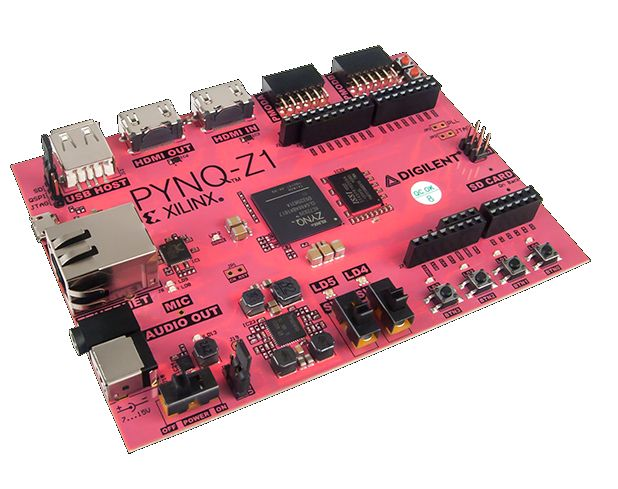
\includegraphics[width=10cm]{4_PYNQ.jpg}
	\caption{Platforma PYNQ z układem Zynq SoC XC7Z020 w centrum}
	\label{fig:PYNQ}
\end{figure}
%TODO Po takim wstępnie powinien nastąpić krótki opis układu Zynq, schemat, omówienie części PS i PL oraz omówinie platfomry PYNQ - zdjęcie... %ODP OK

\section{Tor wizyjny w części PL} %TODO w czści PL ? %ODP OK
\label{sec:counter}


%TODO ???  trzeba zacząć prosto. Podstawowym komponentem... %ODP OK
Podstawowym komponentem toru wizyjnego jest moduł odbierający sygnał wideo z zewnętrznego źródła -- w tym wypadku poprzez port HDMI - i poprawne zdekodowanie go do podstawowej, użytecznej przestrzeni barw RGB. 
Taki zestaw sygnałów może być w prosty sposób wykorzystany w tworzonych algorytmach. %TODO może zostać wykorzystane %ODP OK
Opcjonalne i zalecane jest również wyprowadzenie przetworzonego sygnału RGB na monitor, co pozwoli zweryfikować poprawność tworzonej architektury. 
Wyżej opisany szkielet został stworzony w tzw. \textit{Block Designie}, a poza modułami firmy Xilinx wykorzystano konwertery DVI$\rightarrow$RGB oraz RGB$\rightarrow$DVI dostarczone przez firmę Digilent -- producenta zestawu PYNQ. 
Ponadto, podstawowym zegarem systemu jest dostarczany z karty PYNQ zegar o częstotliwości $125$MHz, na bazie którego powstaje szereg pozostałych zegarów. %TODO a ten radiowy to co i skąd ? Też w tej początkowej koncepcji to powinno być opisane... %ODP pozbyłem się tu informacji o czymkolwiek niezwiązanym z torem wizyjnym
 
W zadaniu śledzenia i detekcji zdecydowanie najważniejszym parametrem jest częstotliwość próbkowania sygnału wideo ze względu na potrzebę analizy jak najmniejszych ruchów obiektu. Kolejnym parametrem jest rozdzielczość - obiekt na obrazie o wyższej rozdzielczości będzie opisywany większą ilością pikseli, jednak niekorzystnie wpływa to na zużycie zasobów układu - wymagane jest osiągnięcie pewnego kompromisu. Z tego względu założono, że transmisja z kamery i przetwarzanie wideo będzie się odbywać w oparciu o standard \textit{720p/60fps}.%TODO napisać dlaczego %ODP OK

Sygnały wideo, które można wyodrębnić po zdekodowaniu, to:
\begin{itemize}
	\item zegar taktujący pikseli ($74.25$MHz),
	\item kolor czerwony R (8 bitów),
	\item kolor zielony G (8 bitów),
	\item kolor niebieski B (8 bitów),
	\item synchronizacja pozioma -- poziom wysoki sygnalizuje koniec poziomej linii,
	\item synchronizacja pionowa -- poziom wysoki sygnalizuje koniec klatki obrazu,
	\item sygnał aktywny -- poziom wysoki sygnalizuje obecność poprawnego piksela.
\end{itemize}

Uwzględniając narzut dany przez sygnały sterujące, ostateczna częstotliwość taktowania piksela wynosi w tym przypadku $74.25$MHz. 
To właśnie ten zegar, nazywany dalej w pracy \textit{\boldmath pixel\char`_clk}, steruje pracą modułów odpowiadających za potokowe przetwarzanie obrazów w części PL. %TODO raczej steruje pracą modułów odpowiadających za %ODP OK
Poniższa ilustracja przedstawia zapis klatki z sygnałami sterującymi, gdzie jednostką jest cykl zegara taktującego piksel. 

\begin{figure}[h]
	\centering
	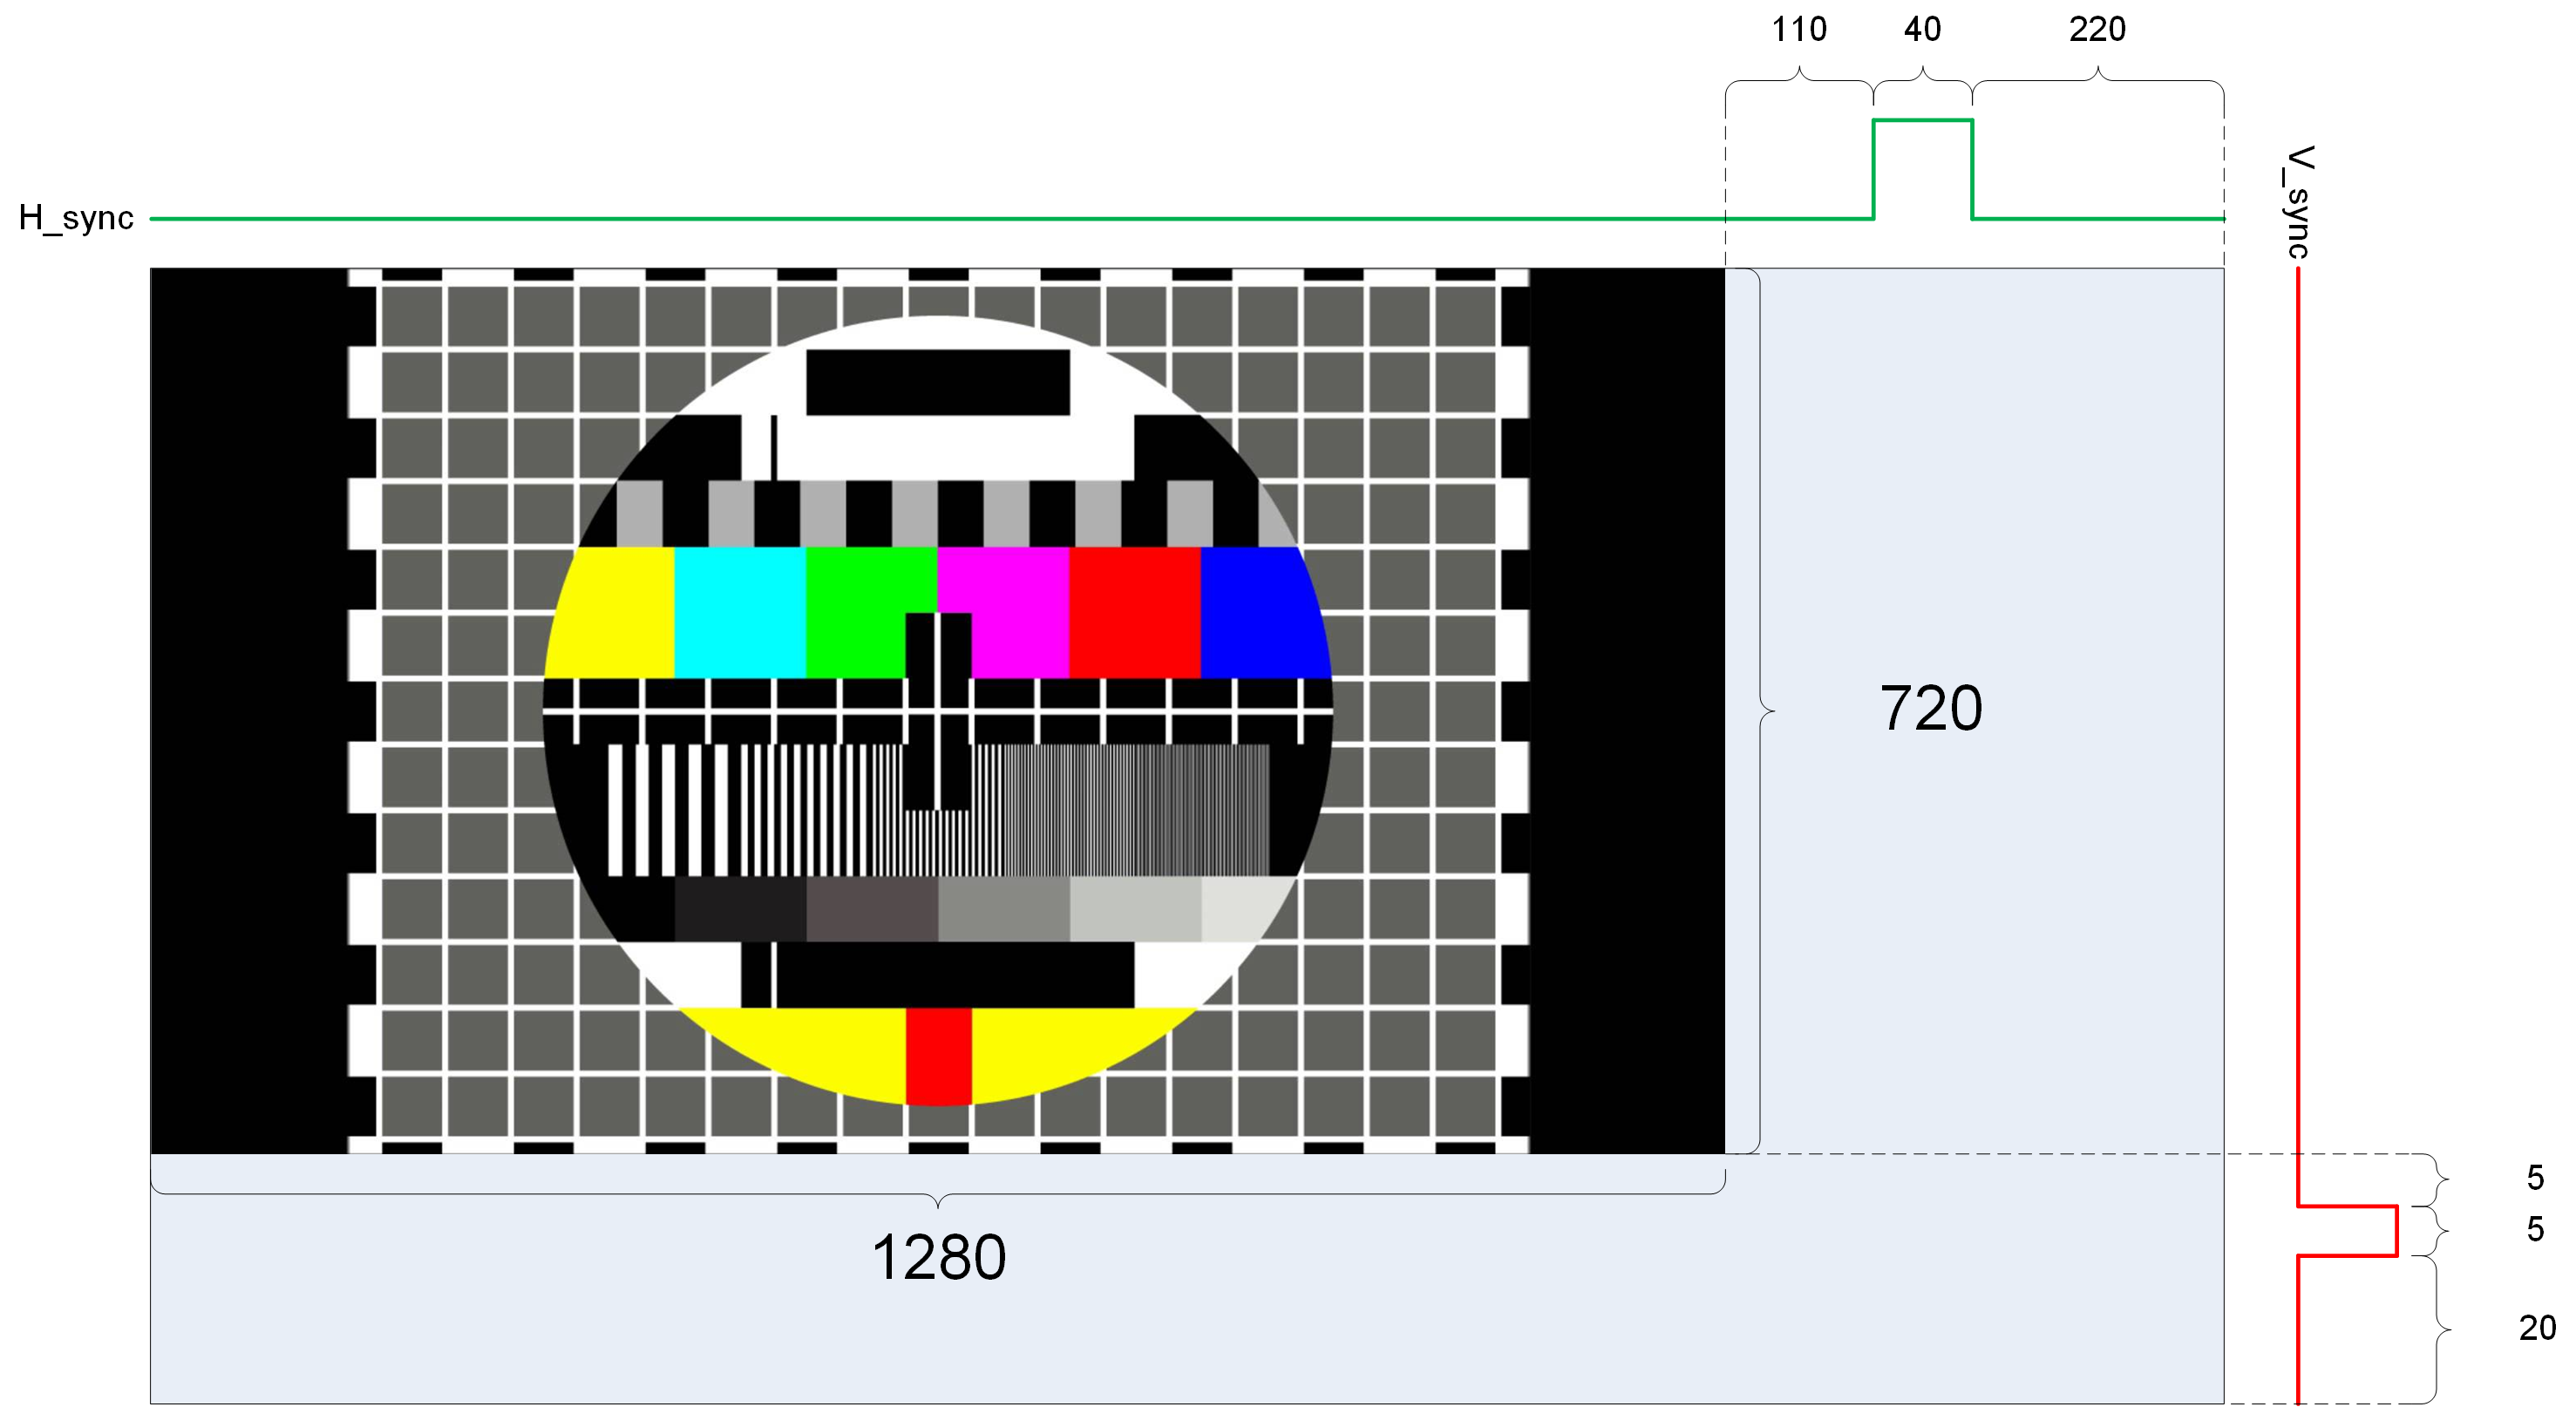
\includegraphics[width=17cm]{4_720p.png}
	\caption{Schemat zapisu klatki w rozdzielczości $720p$}
	\label{fig:720_frame}
\end{figure}

Algorytmy opisane w dalszej części pracy będą często posiłkować się informacją o aktualnym położeniu piksela na właściwym obrazie. 
Stworzono w tym celu licznik obliczający tę pozycję dla osi pionowej i poziomej w oparciu o długości trwania sygnałów kontrolnych z rysunku \ref{fig:720_frame}. 

 
\section{Implementacja algorytmu MeanShift} %TODO Implementacja %ODP OK

Działanie algorytmu MeanShift rozpoczyna się po otrzymaniu sygnału \textit{meanshift\_en} i polega na zdefiniowaniu wzorca, na bazie którego obliczana i zapisywana jest funkcja gęstości prawdopodobieństwa. Następnie porównuje się ją z funkcjami gęstości prawdopodobieństwa kandydatów uzyskanych w kolejnych ramkach obrazu. Na tej podstawie obliczany jest wektor MeanShift, który określa przesunięcie kandydata i jednocześnie obszar następnych poszukiwań.

Pracując nad implementacją, istotne stało się określenie wielkości obszaru śledzonego, który ma być zapisywany z każdej klatki obrazu na podstawie materiału wideo w przestrzeni barw HSV.
Uwzględniając parametry optyczne kamery, jak i rozdzielczość wejściową materiału wideo, podjęto decyzję o śledzeniu obszaru o wymiarach $100 \times 100$ pikseli i ograniczeniu jego otoczenia (czyli możliwości ruchu obiektu pomiędzy klatkami) do 15 pikseli w każdym kierunku.
Po zakończeniu zapisu fragmentu o wymiarach $130 \times 130$, obliczana jest funkcja gęstości prawdopodobieństwa. Tworzona jest ona w oparciu o jądro i jego gradient, które wygenerowano w procesie inicjalizacji. Ostatnim etapem jest obliczenie podobieństwa i określenie przesunięcia obszaru. Algorytm wykonuje ostatnie etapy w sposób iteracyjny, tj. powiększa precyzję przesunięcia śledzonego obszaru, wykorzystując zapisane sąsiedztwo obszaru w celu obliczenia aktualnej funkcji gęstości prawdopodobieństwa. Po określonej ilości iteracji podejmowana jest akwizycja obszaru kandydata z kolejnej klatki.
Analizując możliwości pracy układu w oparciu o testy symulacyjne okazało się, że algorytm jest w stanie pracować z częstotliwością \textit{60Hz}. Może bowiem przetworzyć rozpatrywany fragment z bieżącej klatki obrazu w czasie ok. 4ms, co przy okresie trwania ramki wynoszącym 16.(6)ms  pozwala zakończyć analizę przed zapisem obszaru z kolejnej ramki.  %TODO przedstawić tą analizę... %ODP OK
Ogólny schemat blokowy jest przedstawiony na rysunku \ref{fig:MS_scheme}.
\begin{figure}[h]
	\centering
	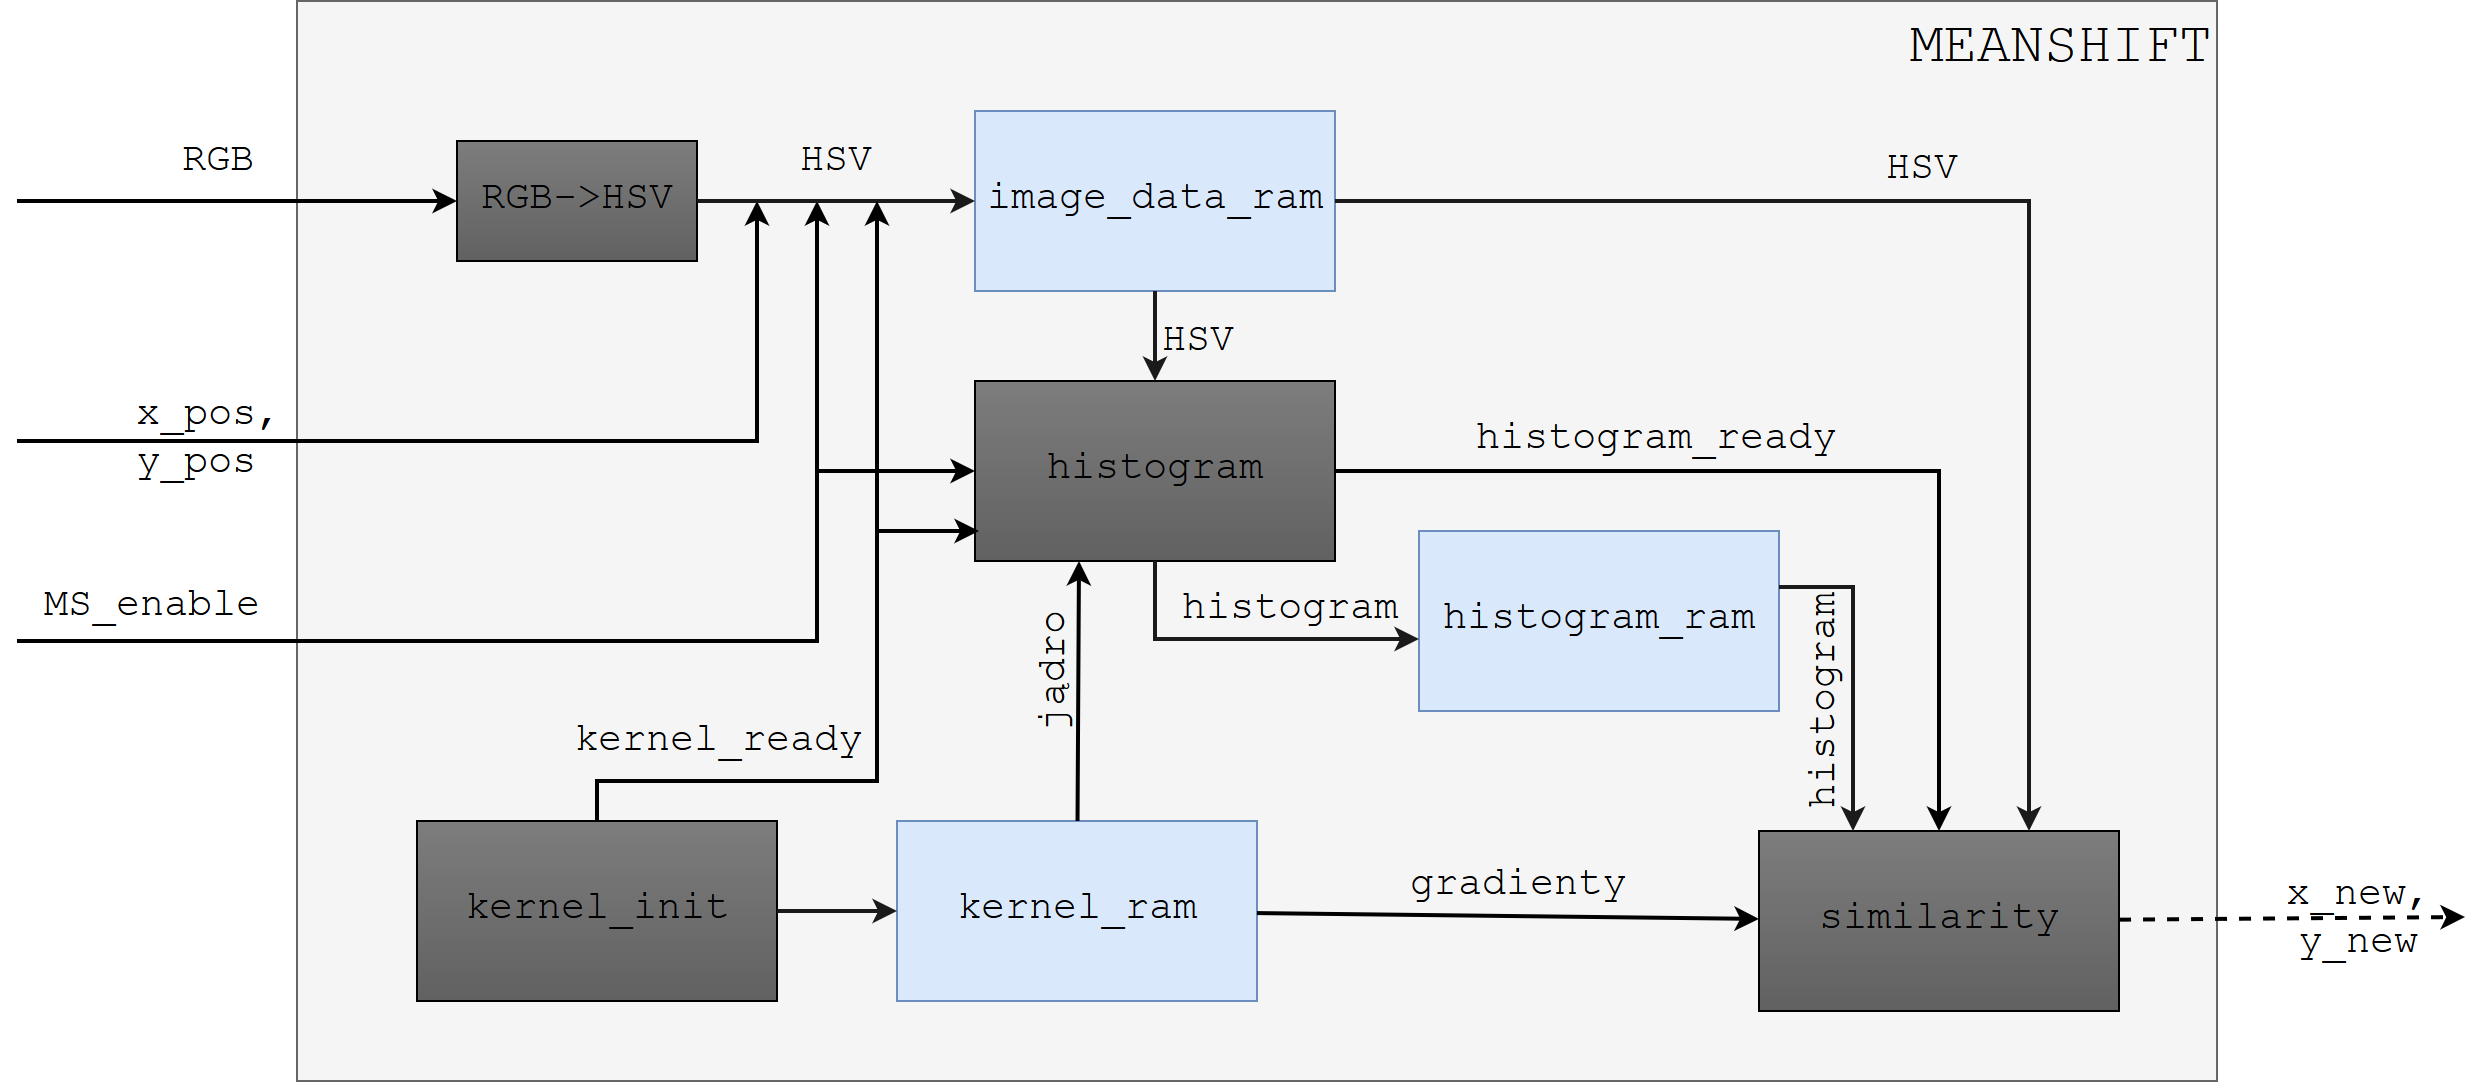
\includegraphics[width=16cm]{Meanshift.png}
	\captionsetup{justification=centering,margin=1cm}
	\caption{Schemat blokowy przedstawiający zależności pomiędzy modułami algorytmu MeanShift}
	\label{fig:MS_scheme}
\end{figure}

%TODO  Tu opisać koncepcję ralizacji...  %ODP OK

\subsection{Konwersja przestrzeni barw RGB->HSV}
%TODO To dać w subsection %ODP OK

Wstępnym etapem toru wizyjnego wewnątrz algorytmu MeanShift jest konwersja przestrzeni barw, realizowana zgodnie ze wzorami \eqref{HSV_first}--\eqref{HSV_last} w module \textit{rgb2hsv}. %TODO na drodze danych -> potoczne %ODP OK
Moduł działa w trybie potokowym pracując na zegarze \textit{pixel\char`_clk} i odpowiednio opóźnia wszystkie sygnały sterujące, co jest istotnym warunkiem poprawnego rozpoznawania odpowiednich pikseli w dalszych etapach przetwarzania.
Dane te są na bieżąco dostarczane do modułu \textit{Meanshift}, realizującego główną część zadań. 

\subsection{Inicjalizacja}

Mimo, że właściwe działanie algorytmu ma miejsce po otrzymaniu sygnału zewnętrznego (\textit{algorithm\char`_en}), wymaga on wcześniejszej inicjalizacji -- odbywa się ona tuż po zaprogramowaniu części PL układu Zynq. %TODO części PL układu Zynq ? %ODP OK
W głównej mierze jest ona związana z obliczeniem jądra i jego gradientów. 
Dane te, wykorzystywane potem w charakterze informacji tylko do odczytu, muszą tu być zapisane w dość uporządkowany sposób. 
Najlepiej nadaje się do tego konfigurowalna pamięć BRAM. 
Powinna ona przechowywać informacje dla wszystkich elementów obszaru, to jest 10000 pól. 
Jej ostateczną organizację przedstawia tabela \ref{tab:kerBRAM}. W kolumnie „Format” litera \textit{U} oznacza liczbę bez znaku, natomiast \textit{S} uwzględnia znak. Kropka oddziela dwie wartości, które określają liczbę bitów przyporządkowanych odpowiednio części całkowitej i ułamkowej.
\newcolumntype{P}[1]{>{\centering\arraybackslash}p{#1}}
\begin{table}[h]
\centering
\caption{Organizacja pamięci BRAM \textit{kernel\char`_ram}}
\begin{tabular}{|P{5cm} |P{3cm} |P{2.5cm}|}

\hline
\rowcolor{lightgray} Informacja & Adres rejestru & Format \\ 
Jądro: $K(||P-P'(x,y)||)$				& 0:9999		& U3.15\\ 
\hline
Gradienty: $g_x$, $g_y$		& 10000:19999	& S0.11, S0.11\\ 
\hline
Norma: $\sqrt{g_x^2+g_y^2}$	& 20000:29999	& U0.11\\ \hline
\end{tabular}

\label{tab:kerBRAM}
\end{table}
%TODO wypda objaśnić kolumnę format %ODP OK
\newline
Warto nadmienić, że zestaw informacji związanych z konkretnym pikselem w obszarze 100x100 opisują rejestry pod adresami:
\begin{equation}
\{100y+x, 10000+100y+x, 20000+100y+x\}, x,y=0..99,
\end{equation}
Ułatwia to zaprogramowanie dostępu do tych danych. %TODO raczej Ułatwia zaprogramowanie dostępu... %ODP OK
By umożliwić odczyt obydwu gradientów w jednym cyklu zegara, zagregowano je w wektor o długości rejestru, tj. 18 bitów. 
Obserwacje poczynione na zapisie gradientów w symulacji dowiodły jednak, że ich wartości są na tyle małe, że 3 najstarsze bity ułamkowe są zawsze równe bitowi znaku. Przykładowo, wartość $0.01$ w formacie S0.11 ma postać $12'b111111011000$. Dysponując $18/2=9$ bitami na gradient można było rozszerzyć precyzję informacji pomijając te 3 nieistotne bity i zapisując ją w pamięci w notacji S0.11, a nie S0.8 -- co pozytywnie wpływa do dokładność obliczeń. Należy pamiętać jednak o tym, by odczyt z rejestru przechowującego gradienty dołączył te 3 bity do wartości przed rozpoczęciem jakichkolwiek obliczeń. %TODO trochę to niejasne -> opisać jak uzyskano ostateczną wartość %ODP OK

Pierwszym etapem inicjalizacji jest obliczenie jądra o wymiarach $100\times 100$. Proces ten przebiega iteracyjnie, budując kolejne warstwy jądra \ref{fig:kernel} w 49 powtórzeniach (bok obszaru -1). Wartością dodawaną do odpowiednich elementóW jądra jest $1/100/2=0.02$, zapisywana w formacie U3.15 jako $0.019989013671875$. Algorytm przechodzi przez 3 zagnieżdżone pętle, przemieszczając się po komórkach jądra \textit{\{x,y\}} i kolejnych warstwach \textit{z}. Schemat \ref{fig:kernel_build} przedstawia przebieg algorytmu. Główny warunek może wydawać się wyzwaniem, jednak wyrażenia typu $W/2$, $H/2$ wymagają jedynie przesunięcia wektora o 1 bit w prawo. Nie zmienia to faktu, że implementacja obliczeń wymaga uwzględnienia odpowiednich opóźnień, a następnie synchronizacji z odczytem i zapisem danego rejestru jądra.
\begin{figure}[h]
	\centering
	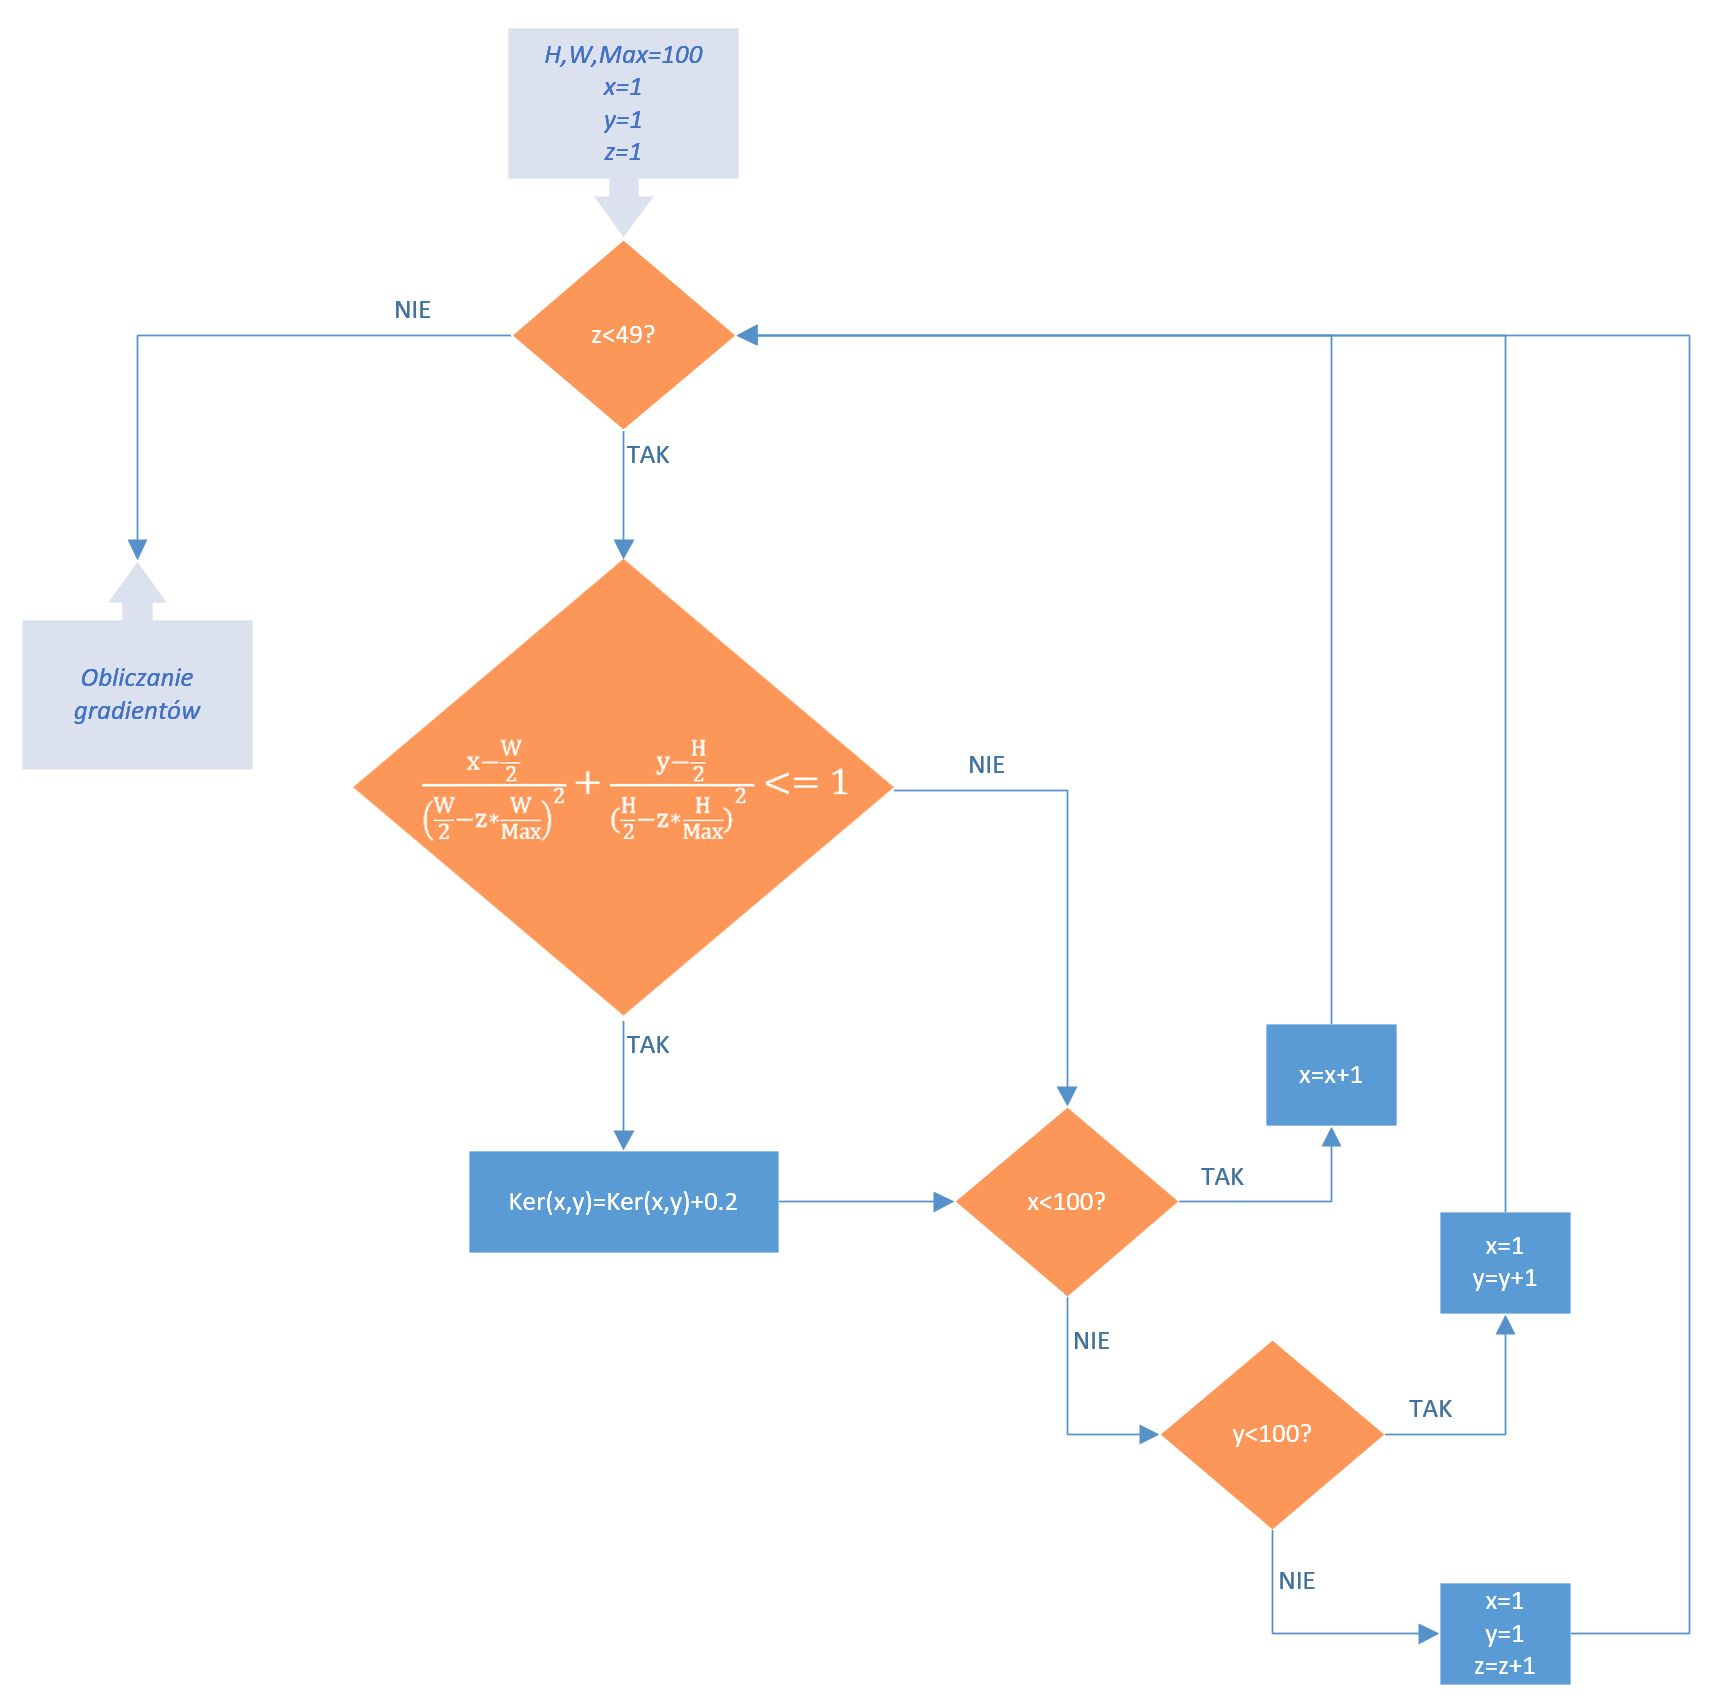
\includegraphics[width=15cm]{4_kernel.jpg}
	\caption{Proces tworzenia jądra obrazu}
	\label{fig:kernel_build}
\end{figure}

Kolejnym etapem jest obliczenie gradientów i ich normy na podstawie gotowego jądra. Dla każdego elementu odczytywane są wartości 4 sąsiadów i kalkulowane gradienty przy użyciu masek: $[1,0,-1]$ oraz $[1,0,-1]^T$. W przypadku sytuacji brzegowych niedostępny sąsiad zostaje zastąpiony rozpatrywanym elementem, a wartość gradientu jest przesuwana o jeden bit w lewo (dwukrotnie zmniejszona odległość pomiędzy obiektami skutkuje dwukrotnym powiększeniem wyniku ilorazu różnicowego).  Na tej podstawie obliczana jest norma gradientu, która wymaga zastosowania dwóch mnożarek i pierwiastkującego bloku CORDIC. Jest to proces na tyle długi, że po zapisie gradientów w pamięci zdecydowano się przejść do kolejnych elementów jądra, jedynie zapamiętując adres rejestru, w którym gotowa wartość normy powinna być zapisana.

Po zebraniu kompletu danych ustawiana jest flaga \textit{kernel\char`_rom\char`_ready}, której obecność sygnalizuje gotowość uruchomienia właściwej części algorytmu. 
Jak stwierdzono w oparciu o symulacje, w rzeczywistości inicjalizacja pamięci \textit{kernel\char`_rom} trwa około 5ms, jest to zatem pomijalnie krótki czas, niewpływający na funkcjonalność (<1 klatka obrazu).


%TODO no dobra, ale to jest jakoś liczone nie ? przecież nie jest to hard-coded. Czyli proszę opisać też elementy to obliczające. %ODP OK, opisano i wrzucono schemat

\subsection{Zapis obszaru wideo}
\label{ssec:savideo}
%TODO żeby to było jasne, to gdzieś wcześniej - na początku, trzeba opisać koncepcję realizacji tego modułu. %ODP OK

Na szerszy opis zasługuje sposób zapisu informacji z obrazu, należy bowiem tymczasowo zapamiętać wartości pikseli $H$, na których obliczenia będą kilkukrotnie wykonywane. 
Dużym obciążeniem dla zasobów układu byłaby próba zapisania całych klatek -- pojedyncza wymagałaby: $1280\cdot720\cdot9\text{b} = 1.037$MB dostępnego miejsca. 
Z tego względu postanowiono zapisywać jedynie obszar w aktualnym położeniu obiektu, z dodatkowym sąsiedztwem 15 pikseli z każdej strony. Szerokość sąsiedztwa dobrano metodą doświadczalną, uwzględniając maksymalne przemieszczenia obiektu pomiędzy kolejnymi klatkami i ograniczenia związane z zasobami.
W procesie zapisu uwzględniono zabezpieczenie na wypadek próby wyjścia poza przestrzeń obrazu. Opiera się na sprawdzeniu pozycji środka obszaru względem ramki obrazu - minimalna odległość od każdej krawędzi to $65$. Zabezpieczenie to funkcjonuje również w samym algorytmie, utrzymując ostateczną pozycję obszaru wewnątrz dozwolonego wycinka ramki. %TODO za długie zdanie. to zabezpieczenie to osobnego zdania i opisać lepiej %ODP OK
%Sąsiedztwo to pozwoli algorytmowi wskazać przesunięcie obszaru najbardziej zbliżone do faktycznego ruchu obiektu. 
%TODO styl. algorytmowi i w sumie niejanse. %ODP zakomentowano, parę linijek wyżej jest lepsze wytłumaczenie


Proces śledzenia musi poprawnie określić położenie aktualnego, \enquote{użytecznego} piksela, a także rozpoznać początek kolejnej klatki. 
Jest to możliwe poprzez stworzenie logiki opierającej się na licznikach: horyzontalnym i wertykalnym, która wykrywa zbocza sygnałów sterujących. %TODO analizującą -- źle brzmi i też coś nie pasuje %ODP OK
Liczniki wykorzystują informacje przedstawione na rysunku \ref{fig:720_frame}; zliczają odpowiednio do wartości 1280 oraz 720.

Otrzymanie sygnału \textit{algorithm\char`_en} inicjuje realizację algorytmu. 
Istotne jest, aby w momencie pojawienia się tego sygnału, w obszarze zdefiniowanym jako startowy (domyślnie środek obrazu) znajdował się śledzony obiekt. 
Obszar ten, będący od teraz wzorcem, jest zatrzaskiwany na najbliższej pełnej klatce obrazu. 
Następnie obliczana jest funkcja gęstości prawdopodobieństwa, opisana w podrozdziale \ref{ssec:fgp}. %TODO sekcja -> (pod)rozdzał (to jest złe słowo w PL) %ODP OK

Wartości pikseli -- linia po linii --  są przechowywane w module BRAM działającym w trybie True Dual Port, \textit{image\char`_data\char`_ram}.
Dzięki temu możliwy jest jednoczesny zapis/odczyt pod warunkiem, że porty nie pracują jednocześnie na tym samym adresie. 
Ze względu na konieczność posiadania kompletnego fragmentu obszaru i możliwość zapisu kolejnego, pamięć zdolna jest pomieścić 2 obszary z ostatnich klatek, każdy o wymiarach $130 \times 130$: łącznie 33800 adresów. 
Zamiennie, co klatkę, wykonywany jest zapis najnowszych danych do jednej połowy przestrzeni, i przetwarzanie (odczyt) drugiej \ref{tab:imageBRAM}. 
%Warto jednak zwrócić uwagę na rozbieżność w szybkości obu tych procesów --  o ile zapis działa synchronicznie z zegarem piksela, \textit{pixel\char`_clk}, to algorytm będzie odczytywał dane z prędkością \textit{\boldmath calc\char`_clk}, celowo taktowanego innym zegarem (100MHz).
%TODO pozwala to na ?? %ODP True dual port pozwala na dostęp do pamięci na dwóch różnych zegarach, ale rzeczywiście jakiś czas temu cofnąłem prędkość działania meanshift w całości do PixelClk, bo w zupełności wystarcza. Zakomentowałem to zdanie.

\newcolumntype{P}[1]{>{\centering\arraybackslash}p{#1}}
\begin{table}[h]
	\centering
	\caption{Organizacja pamięci BRAM \textit{image\char`_data\char`_ram}}
	\begin{tabular}{|P{4cm} |P{3cm} |P{2cm}|}
		
		\hline
		\rowcolor{lightgray} Informacja & Adres rejestru & Format \\ 
		Klatka $t\%2==0$			& 0:16899		& U9\\ 
		\hline
		Klatka $t\%2==1$		& 16900:33799	& U9\\ 
		\hline
	\end{tabular}

	\label{tab:imageBRAM}
\end{table}
%TODO brak referencji do tabeli w tekście %ODP OK
%\newline

%TODO Jednego nie rozumiem. Zatrzaskiwany jest też wzorzec, czy tylko są dla niego obliczany histogram.
%ODP Zatrzaskiwany jest histogram wzorca, do bieżącego śledzenia wymagane są jedynie wartości pikseli kandydata.
\subsection{Funkcja gęstości prawdopodobieństwa}
\label{ssec:fgp}

Wartość funkcji gęstości prawdopodobieństwa jest inaczej wartością histogramu dla danej barwy piksela ($H$ z zakresu 0-359). 
W tym celu utworzono pamięć BRAM, która przechowuje dwa histogramy dla wzorca oraz kandydata -- w sumie 720 rejestrów \ref{tab:histBRAM}. 
\newcolumntype{P}[1]{>{\centering\arraybackslash}p{#1}}
\begin{table}[h]
	\centering
	\caption{Organizacja pamięci BRAM \textit{histogram\char`_ram}}
	\begin{tabular}{|P{4cm} |P{3cm} |P{2cm}|}
		
		\hline
		\rowcolor{lightgray} Informacja & Adres rejestru & Format \\ 
		Histogram wzorca			& 0:359		& U10.15\\ 
		\hline
		Histogram kandydata		& 360:719	& U10.15\\ 
		\hline
	\end{tabular}

	\label{tab:histBRAM}
\end{table}
%TODO brak ref do tab %ODP OK
\newline
Histogram wzorca jest tworzony raz, w oparciu o pierwszy obraz; kolejne histogramy są związane z kandydatem i zostają zapisane w górnej połowie adresowej ($H+360$). 
Wartość piksela, umożliwiając dostęp do odpowiedniego rejestru pamięci, pozwala na odczyt dotychczasowej wartości przedziału histogramu i przygotowanie go do aktualizacji. Z kolei współrzędne piksela w odniesieniu do obszaru $100 \times 100$ są wykorzystywane do odczytu elementu jądra. Przedział histogramu jest aktualizowany zapisem sumy obu wartości.  %TODO styl. piksel nie dodaje. + lepiej to opisać ? moduł DSP użyty , %ODP OK
Format rejestrów pamięci \textit{histogram\char`_ram} pozwala na zapis wartości w formacie U10.15, czyli w zakresie [0:1023.99997]. %TODO też precyzję opisać. %ODP OK
Zdarzają się jednak przypadki, gdy większość pikseli na obszarze (zwłaszcza w centrum -- miejscu największych wartości jądra) jest jednokolorowa, co może skutkować przekroczeniem dopuszczalnych wartości dla rejestru. %TODO bez próbą %ODP OK
Chroni przed tym dodatkowy fragment logiki, który wykrywając takie zdarzenie, pozostawia rejestr z maksymalną wartością.

Wartość pikseli jest odczytywana bezpośrednio z pamięci przechowującej analizowany obszar, opisanej w podrozdziale \ref{ssec:savideo}. 
Do obliczenia histogramu wymaganych jest jedynie $100\times 100$ pikseli, pozostałe (sąsiedztwo) należy zignorować. %TODO to jest trochę niejasne %ODP OK
Wartości \textit{offset\char`_X} oraz \textit{offset\char`_Y} określają pozycję pierwszego analizowanego piksela (w lewym górnym rogu). Startując z tego miejsca, praca liczników \textit{H\char`_count} oraz \textit{W\char`_count} pomaga w zebraniu jedynie 100 pikseli ze 100 linii. %TODO styl. rejestry obliczają. %ODP OK
Przykładowo, obliczając po raz pierwszy histogram dla ostatnio zapisanej klatki zmienne \textit{offset\char`_X} i \textit{offset\char`_Y} mają wartości domyślne $(15,15)$. 
Oznacza to, że z zapisanego obszaru o wymiarach $130\times 130$ należy odczytać jego środek, a koordynaty pierwszego piksela będą wynosić $(15,15)$. W kolejnych iteracjach algorytmu dla tej samej klatki obrazu zmienne mogą przyjąć inne wartości, tworząc w efekcie funkcję gęstości prawdopodobieństwa odpowiadającą nowemu fragmentowi obszaru $100\times 100$. %TODO czyli w środku rozważanego obszaru ? %ODP tak, poprawiono
Zakres dopuszczalnych wartości dla każdej z tych zmiennych to $<0,29>$. 

Po przejściu przez wszystkie piksele obszaru następuje ustawienie flagi \textit{histogram\char`_ready}, gdzie w przypadku przetwarzania klatki-wzorca kolejnym zadaniem jest akwizycja pierwszego kandydata, natomiast dla każdej kolejnej rozpocznie obliczanie funkcji podobieństwa.
Podobnie jak \textit{image\char`_data\char`_ram}, \textit{histogram\char`_ram} działa w trybie True Dual Port. %TODO algroytm przechodzi %ODP OK
Po obliczeniu funkcji gęstości dla aktualnego obszaru, z pamięci jednocześnie są odczytywane wartości funkcji dla wzorca (port A) i kandydata (port B pamięci) -- umożliwiając wykonywanie części dalszych obliczeń w sposób równoległy. %TODO też "jest on w stanie". %ODP OK

%TODO to proszę konktrertnie co jest przez jakie porty... %ODP OK,wskazano porty w zdaniu w zdaniu wyżej

\subsection{Funkcja podobieństwa}

Moduł implementujący kalkulację funkcji podobieństwa (i ostatecznie przesunięcia) obszaru, jest najbardziej złożony w tej części systemu. 
Funkcja podobieństwa, opisana wzorem \eqref{eq:position}, jest obliczana dla każdego piksela w pamięci, należącym do właściwego obszaru (bez sąsiedztwa). %TODO raczej dla każdego piksela %ODP OK

Dla każdego piksela z obszaru $100 \times 100$, którego wartość $H$ jest adresem dla pamięci $histogram\char`_ram$, wczytywana jest wartość funkcji prawdopodobieństwa wzorca i kandydata. 
Moduł oblicza ich iloraz (wzorzec/kandydat) używając bloku Divider Generator (w wersji 5.1) dostarczonego przez firmę Xilinx. %TODO konkretnie %ODP OK
Ze względów optymalizacyjnych obcięto 9 najmłodszych bitów obu wartości, gdyż nie wpływały w większym stopniu na dokładność, a ich pominięcie pozwoliło zmniejszyć latencję modułu. %TODO pozbycie -> pominięcie %ODP OK
Podczas takiego dzielenia logika musi ponadto sprawdzić obecność zera w mianowniku -- wówczas iloraz powinien być zerowany. 
Brak obsługi takiego zdarzenia doprowadziłby do otrzymania ilorazu o trudnej do przewidzenia wartości -- mogłoby to powodować poważne błędy w działaniu algorytmu. 

Gotowy iloraz należy poddać pierwiastkowaniu. 
Moduł obliczający pierwiastek wymaga, by wejście z danymi było liczbą całkowitą lub  też ułamkową -- ale z jednym bitem dla części całkowitej: U1.X. 
W tym celu wynik dzielenia -- liczba w formacie: U16.16 -- została obcięta do U13.11., a następnie ,,wirtualnie'' przesunięta o 12 bitów w prawo, do postaci: U1.23. 
Wynik pierwiastkowania wymaga przesunięcia w lewo już tylko o 6 bitów ($\sqrt{2^{12}}=2^6$), po czym jest obcinany do 16 najbardziej znaczących bitów: U7.9.
Operacje te, mimo że zawiłe, nie wpływają na wynik, lecz gwarantują poprawne działanie modułu \textit{CORDIC} realizującego pierwiastkowanie.

Wartości pierwiastka współtworzyć będą zarówno licznik, jak i mianownik ilorazu wektora MeanShift -- oddzielnie dla przesunięcia pionowego i poziomego. %TODO rozdzielnie -> oddzielnie %ODP OK
Obliczenie iloczynów wymaga pobrania z pamięci \textit{kernel\char`_ram} obu gradientów oraz ich normy. 
Odczyt jest zoptymalizowany pod zminimalizowanie liczby cykli zegara potrzebnych na odczytanie obu wartości i został oparty o maszynę stanu.
Po zakończeniu przetwarzania wszystkich pikseli obszaru $100 \times 100$ (sumowania obliczonych na ich podstawie wartościach) ustawiana jest flaga \textit{div\_enable\_de}, która jest podłączona do modułów realizujących dzielenie w wektorze MeanShift. Otrzymane wyniki dzielenia odpowiadają przesunięciu obszaru śledzenia, należy je jednak znormalizować do postaci całkowitej i upewnić się, że obszar po przesunięciu nadal będzie w całości znajdował się w zapisanym fragmencie o wymiarach $130 \times 130$. Pozwoli to wykonać kolejne iteracje, które mogą poprawić wynik śledzenia. O ile pierwsza iteracja rozpoczyna analizę w środku obszaru, to w trakcie kolejnych informacja o położeniu obszaru wewnątrz $130 \times 130$ jest zapamiętywana przez zmienne \textit{offset\_X} oraz \textit{offset\_Y}.
%TODO no właśnie opisać... %nie przyuważyłem tego braku, dopisano.


%TODO Brakuje schematu blokowego modułów wchodząych w skład algorymtu. Te pamięci, konwersja itp... %ODP Dodano we wstępie


\section{Realizacja algorytmu HOG+SVM}

%TODO Też trzeba zacząć od jakieś koncepcji implementacji. %ODP dodano poniżej

Wymagania stawiane przez system mówią o konieczności rozpoznania osoby wraz z dodatkowym określeniem jej wielkości na ekranie (skala ta pozwoli dość ogólnie wyznaczyć odległość drona od obiektu, co wpłynie na sterowanie maszyny). Jednym z celów jest bowiem utrzymanie stałej odległości od postaci. %TODO w sumie można napisać/powtórzyć, że celem jest utrzymanie stałej odłegłości od pieszego. %ODP OK
Z tego względu implementacja musi wykorzystać tzw. piramidę skal, czyli równoległą detekcję HOG+SVM na serii obrazów o różnych wymiarach. %TODO serii obrazów o różnych wymiarach %ODP OK
Dysponując obrazem o rozdzielczości $1280 \times720$, należy przeskalować go do kilku mniejszych, a następnie przeprowadzić na nich opisane wcześniej operacje wyliczenia wektora cech i sklasyfikować go przy użyciu SVM. 
Odpowiednia lokalizacja postaci (i jej odległość od kamery) zostanie wybrana na podstawie najlepszego \textbf{pozytywnego} wyniku klasyfikacji, w oparciu o wartość $r$ \eqref{eq:HOG_classification}. %TODO \eqref do stosownego równania %ODP OK

Algorytm ten może rozpocząć działanie jedynie na pełnej klatce obrazu, zatem stworzono mechanizm, który niezależnie od momentu pojawienia się sygnału wyzwalającego pracę algorytmu będzie oczekiwał na zbocze opadające sygnału synchronizacji pionowej, czyli nową, pełną ramkę. Tylko w takim przypadku gwarantowane jest poprawne działanie algorytmu. %TODO trochę niejasne %ODP OK
Drugim warunkiem jest to, by w momencie nadejścia nowej klatki algorytm nie był w trakcie przetwarzania poprzedniej -- w przeciwnym wypadku histogramy mogłyby być nadpisywane nowymi wartościami. 
Oznacza to jednak, że co druga klatka obrazu będzie pomijana w przetwarzaniu, ograniczając częstotliwość pracy algorytmu do \textit{30Hz}.
%TODO rozumiem, że to nie jest w pełni potokowa implementacja %ODPOstatecznie nie, wymagane byłoby stworzenie drugiego zestawu pamięci dla wektorów cech nieparzystych klatek, a na to nie ma BRAMów

W pierwszej kolejności obraz wejściowy poddawany jest konwersji do skali odcieni szarości. 
Następna w kolei, operacja skalowania do 5 mniejszych obrazów metodą najbliższego sąsiedztwa, jest realizowana potokowo, dzięki czemu można zachować sygnały kontrolne VGA (synchronizację poziomą oraz pionową). %TODO jaka metoda skalowanie, jakie te skale, co Pan rozumie poprzez "na bieżąco". %ODP OK
Na pomniejszonych obrazach obliczane są wektory cech, bazując na komórkach o wielkości $4\times 4$ i blokach o rozmiarze $2\times2$. 
Dysponując określoną liczbą zasobów układu XC7Z020, nie jest możliwa analiza całego obrazu, a jedynie otoczenia aktualnie śledzonego fragmentu.
%TODO no to nie jest prawda, bo da się to zrobić i dla całego obrazu i dla wielu skal - są takie artykułu. Przy czym jest to niewątpliwe dość trudne i wymaga sporo zasobów %O tym wiem, odnosiłem się oczywiście do urządzenia które mam pod ręką - uściśliłem
Musi ono być jednak wystarczająco duże, by klasyfikator miał szansę wybrać jak najlepszą detekcję osoby w jego wnętrzu. 
Jak wspomniano wcześniej, wektor cech tworzony jest na wycinku o rozmiarze $128\times 64$ pikseli. 
Przedstawia to obraz \ref{fig:HOG_mesh}, gdzie taki wycinek zaznaczono zieloną linią. %TODO rzut-> obrazek oraz nie poniższy tylko ref

\begin{figure}[h]
	\centering
	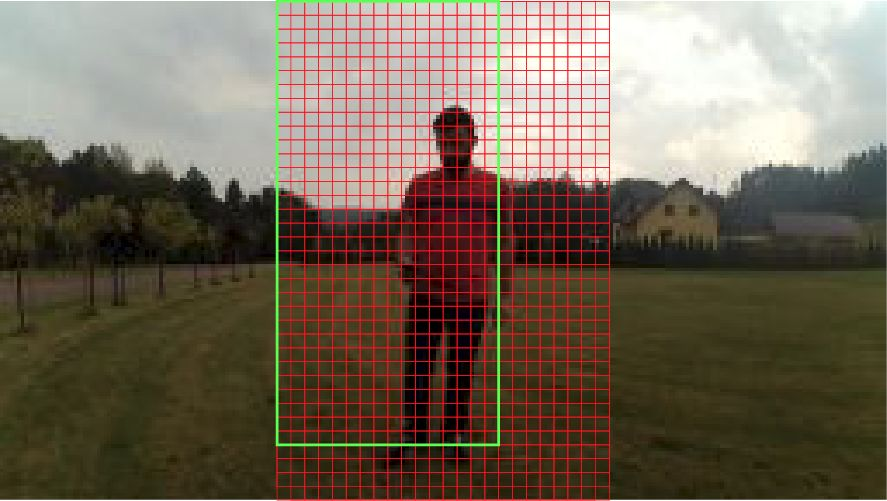
\includegraphics[width=11cm]{4_scaled_hog_example.jpg}
	\caption{Analiza obrazu o rozmiarach $144\times 256$}
	\label{fig:HOG_mesh}
\end{figure}
%\newline

Jeśli algorytm będzie pracował na obszarze $144\times 96$, to zakładając stałe położenie komórek na obrazie (są to kwadraty $4\times4$ wydzielone czerwonymi liniami), powstanie łącznie $5\cdot9=45$ wektorów cech. 
Reszta obrazu zostaje zignorowana. 
Współrzędne centrum obszaru detekcji są określane na początku działania pojedynczej iteracji algorytmu i są natychmiastowo konwertowane do odpowiednich skal obrazu. Po zakończeniu klasyfikacji współrzędne odpowiadające najlepszej detekcji są konwertowane do oryginalnej skali i wykorzystywane podczas analizy kolejnej dostępnej klatki obrazu.

Ogólny schemat blokowy jest przedstawiony na rysunku \ref{fig:HOG_SVM_scheme}.
\begin{figure}[h]
	\centering
	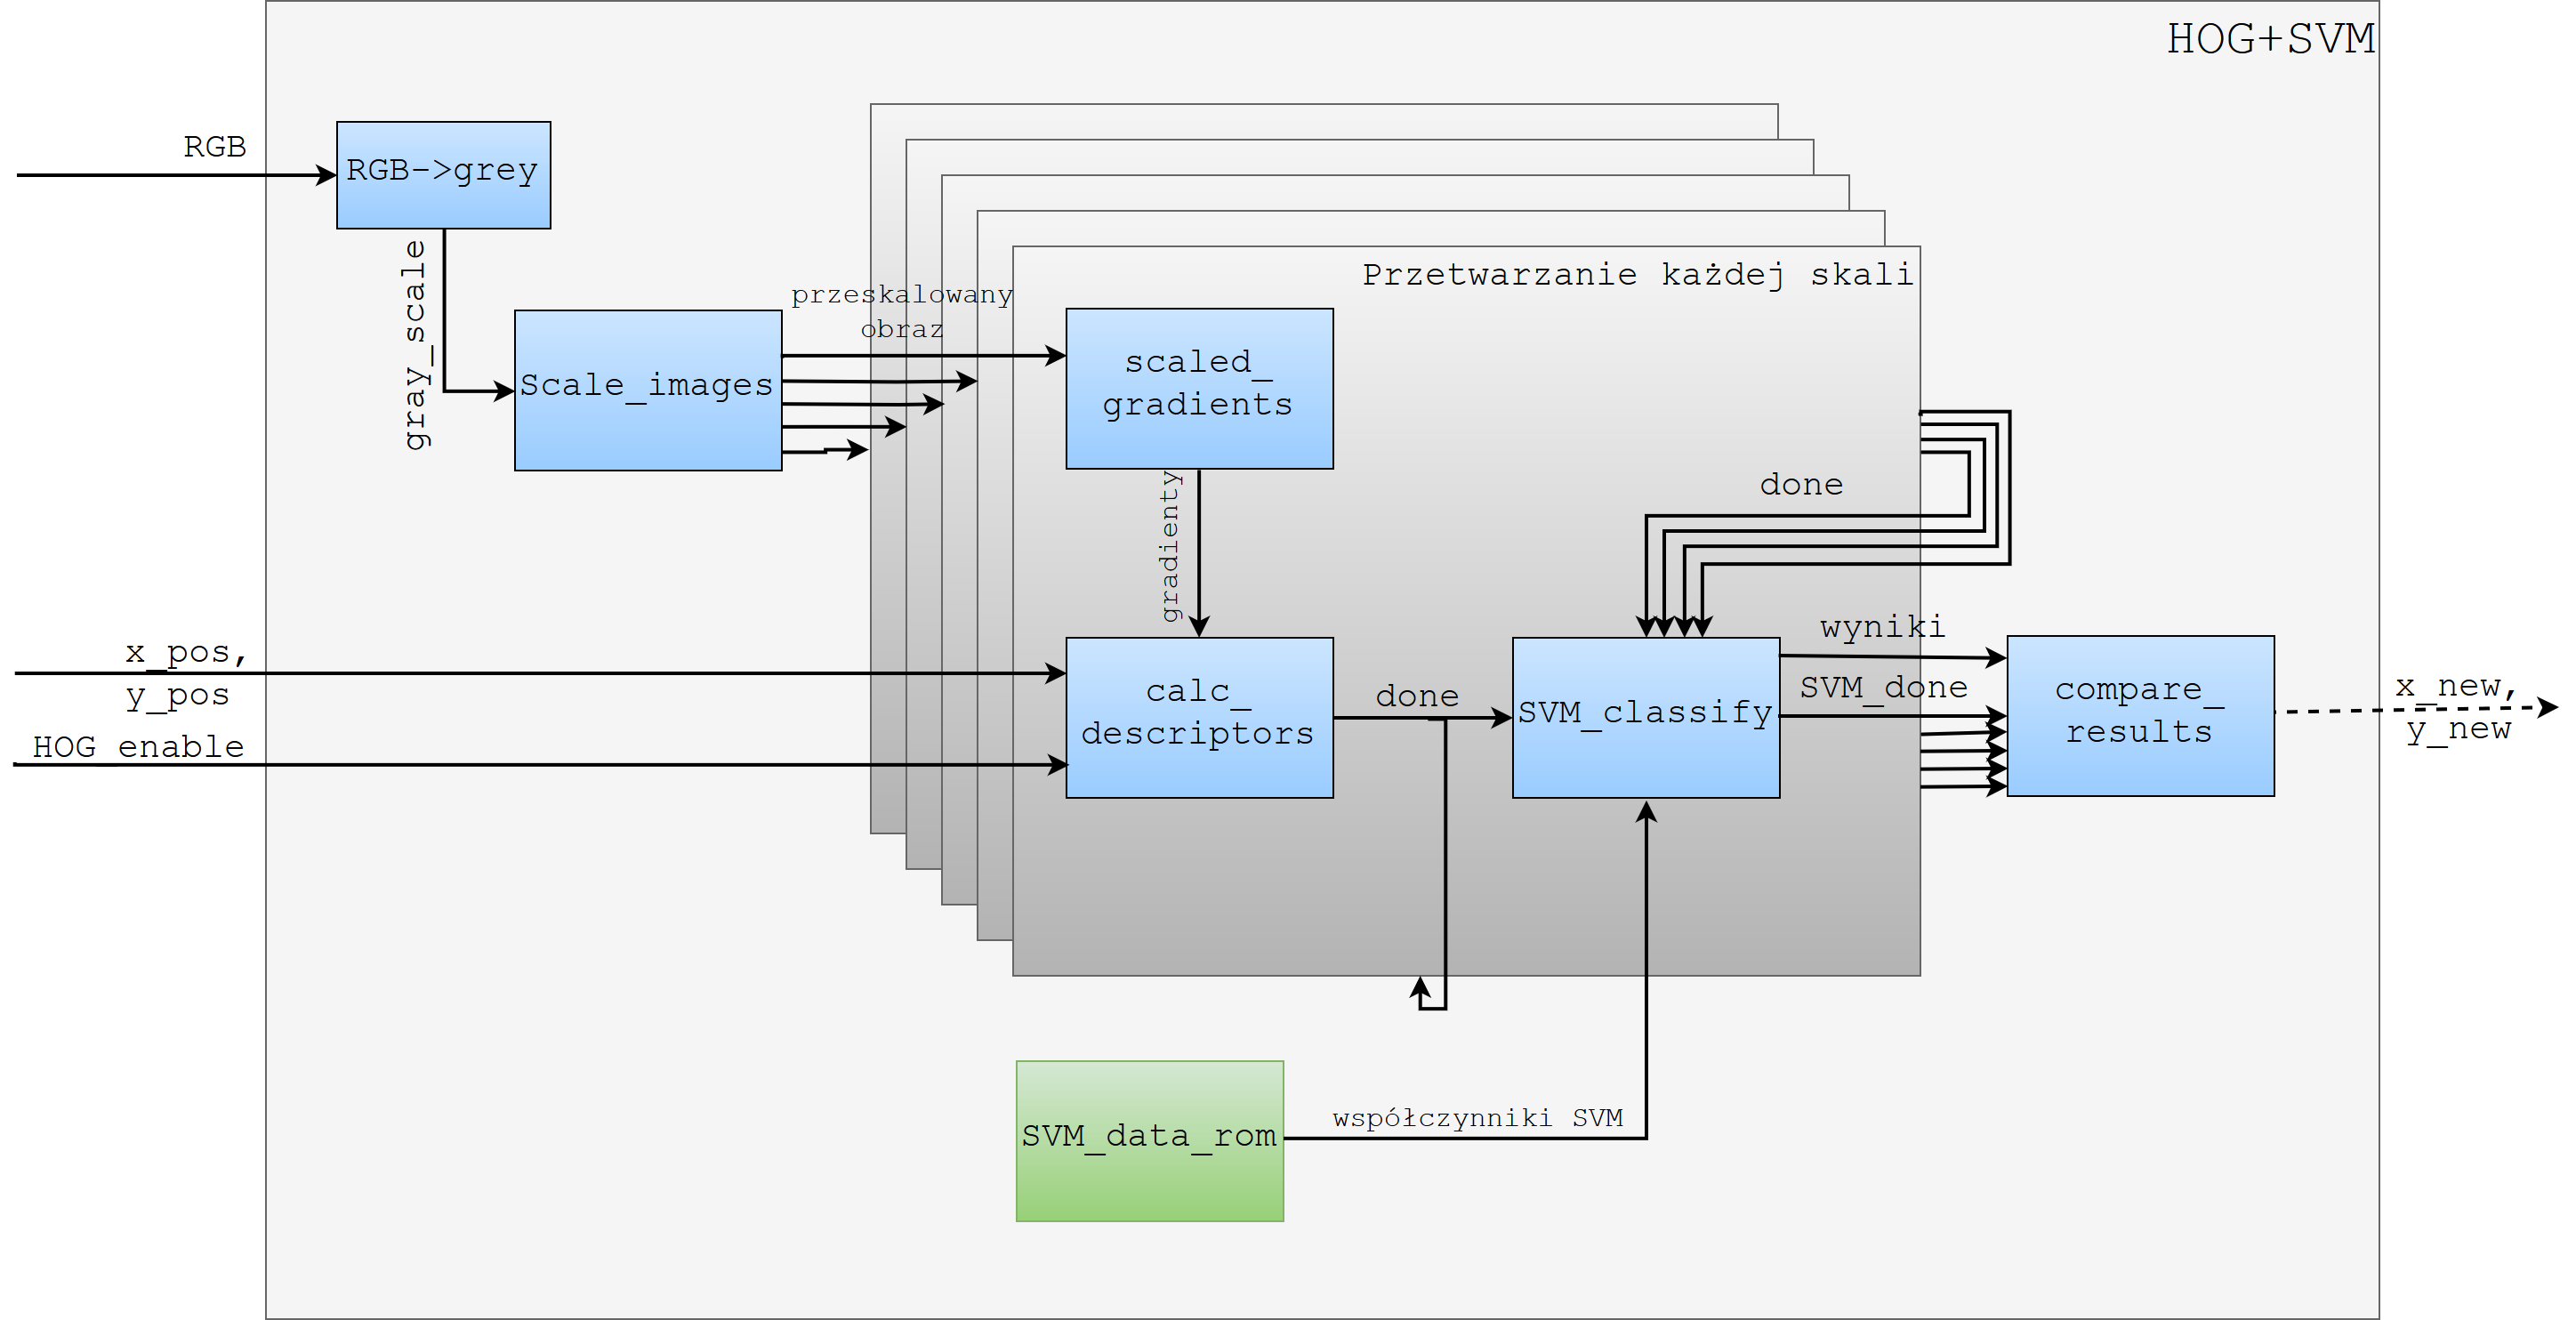
\includegraphics[width=16cm]{HOG_SVM.png}
	\captionsetup{justification=centering,margin=1cm}
	\caption{Schemat blokowy przedstawiający zależności pomiędzy modułami algorytmu HOG+SVM}
	\label{fig:HOG_SVM_scheme}
\end{figure}
\subsection{Konwersja RGB do skali odcieni szarości}

Obraz wejściowy jest poddawany konwersji zgodnie ze wzorem \eqref{eq:rgb2gray}. 
Używane są tu trzy równoległe mnożarki, a suma iloczynów jest zaokrąglana do 8 bitów (do postaci liczby całkowitej z zakresu 0-255).

\subsection{Skalowanie}

Kolejny etap to przeskalowanie obrazu wejściowego. 
Sama idea okazuje się być tym bardziej na miejscu, jeśli wziąć pod uwagę parametry kamery zamontowanej na dronie -- w przypadku tego projektu jest to Xiaomi Yi, urządzenie do zastosowań sportowych i charakteryzujące się dużym kątem widzenia -- 155$^{\circ}$. %TODO myśl dobra, ale styl do zmiany.. %ODP OK
W efekcie osoba oddalająca się od kamery bardzo szybko zmniejszy swoje wymiary na obrazie. 
Materiał $1280\times 720$ pikseli przeskalowano do 5 obrazów przy użyciu następujących skal:
\NumTabs{15}
\begin{itemize}
	\item \textbf{1:  2}\tab{:}\tab{$720\times 1280\rightarrow360\times 640$} pikseli
	\item \textbf{1:2.5}\tab{:}\tab{$720\times 1280\rightarrow288\times 512$} pikseli	
	\item \textbf{1:  3}\tab{:}\tab{$720\times 1280\rightarrow240\times 426$} pikseli
	\item \textbf{1:3.5}\tab{:}\tab{$720\times 1280\rightarrow205\times 365$} pikseli
	\item \textbf{1:  4}\tab{:}\tab{$720\times 1280\rightarrow180\times 320$} pikseli
\end{itemize}

Powyższe wartości pozwalają jednocześnie zachować prostotę implementacji (skale są reprezentowane w formacie U3.1) i z akceptowalnym marginesem błędu określić odległość drona od postaci. %TODO wyraźnie to złe słowo. %ODP OK

Skalowanie przebiega w dość prosty sposób i polega na pomijaniu odpowiednich wierszy lub/i kolumn oryginalnego obrazu. Jeśli założyć, że: %TODO chyba pomijanie odpowiednich/wybranych %ODP OK
\begin{itemize}
	\item $x_i$, $y_i$ -- współrzędne obrazu wejściowego,
	\item $x_o$, $y_o$ -- współrzędne obrazu wyjściowego (przeskalowanego),
	\item $s_c$ -- skala do zastosowania w pionie oraz w poziomie,
\end{itemize}
to przypisanie wartości obrazu wejściowego nastąpi przy jednoczesnym spełnieniu obu poniższych warunków:
\begin{equation}
\label{eq:scaling}
\left.\begin{aligned} 
x_i&==\lfloor s_cx_o\rfloor \\ 
y_i&==\lfloor s_cy_o \rfloor
\end{aligned}\right.
\end{equation}
Po natrafieniu na odpowiedni piksel, oprócz przypisania jego wartości do wyjścia, wystawiony zostanie sygnał sterujący \textit{valid}, bardzo ważny dla dalszej części algorytmu.
Przykład dla kilku pierwszych wartości \textit{x\char`_o} jest widoczny w tabeli \ref{tab:scaling}.
\begin{table}[h]
	\centering
	\captionsetup{justification=centering,margin=1cm}
	\caption{Przykładowy przebieg skalowania dla $s_c=2.5$ wraz z przypisywanymi pikselami wejściowymi}	
	\begin{tabular}{|P{2cm} |P{3cm} |P{2cm}|}	
		\hline
		\rowcolor{lightgray} $x_o$ & $x_is_c$ & $x_i$ \\ 
		1		& 2.5	& 2\\ 
		\hline
		2		& 5		& 5\\ 
		\hline
		3		& 7.5	& 7\\ 
		\hline
		4		& 10	& 10\\ 
		\hline		
	\end{tabular}
	\label{tab:scaling}
\end{table}

Działanie modułu opiera się na stworzeniu dwóch zestawów liczników dla każdej skali. 
Pierwszy zestaw pozwala na określenie indeksów piksela wejściowego ($x_i$, $y_i$) i został opisany w sekcji \ref{sec:counter}. %TODO zdeterminowanie... dziwne słowo w tym kontkeście %ODP spolszczenie angielskiego słowa, poprawione
Drugi zestaw liczników działa zgodnie ze schematem \ref{fig:scaling_sch}. %TODO nie poniższym tylko przedstawionym na rys... %ODP OK 
Oznaczeniem \textit{@PixelClk} opisano proces oczekiwania na kolejne zbocze narastające zegara pikselowego. W momencie pojawienia się sygnału synchronizacji pionowej następuje inicjalizacja liczników koordynatami piksela zlokalizowanego w lewym górnym rogu docelowej klatki skalowanego obrazu. W trakcie otrzymywania kolejnych pikseli na wejściu porównywane są wartości obu liczników - spełniony warunek oznacza wystawienie wartości piksela na wyjście modułu wraz z sygnałem aktywnym. W przeciwnym wypadku sygnał aktywny jest zdejmowany. Obecna na schemacie zmienna \textit{flag} służy do jednorazowych inkrementacji licznika $y_0$ z uwagi na dwie kwestie:
\begin{itemize}
	\item sygnał synchronizacji poziomej jest ustawiany na 40 cykli zegara pikselowego
	\item sygnał synchronizacji poziomej jest obecny po sygnale synchronizacji pionowej a przed nadejściem pierwszego piksela
\end{itemize}   
\begin{figure}[!h]
	\centering
	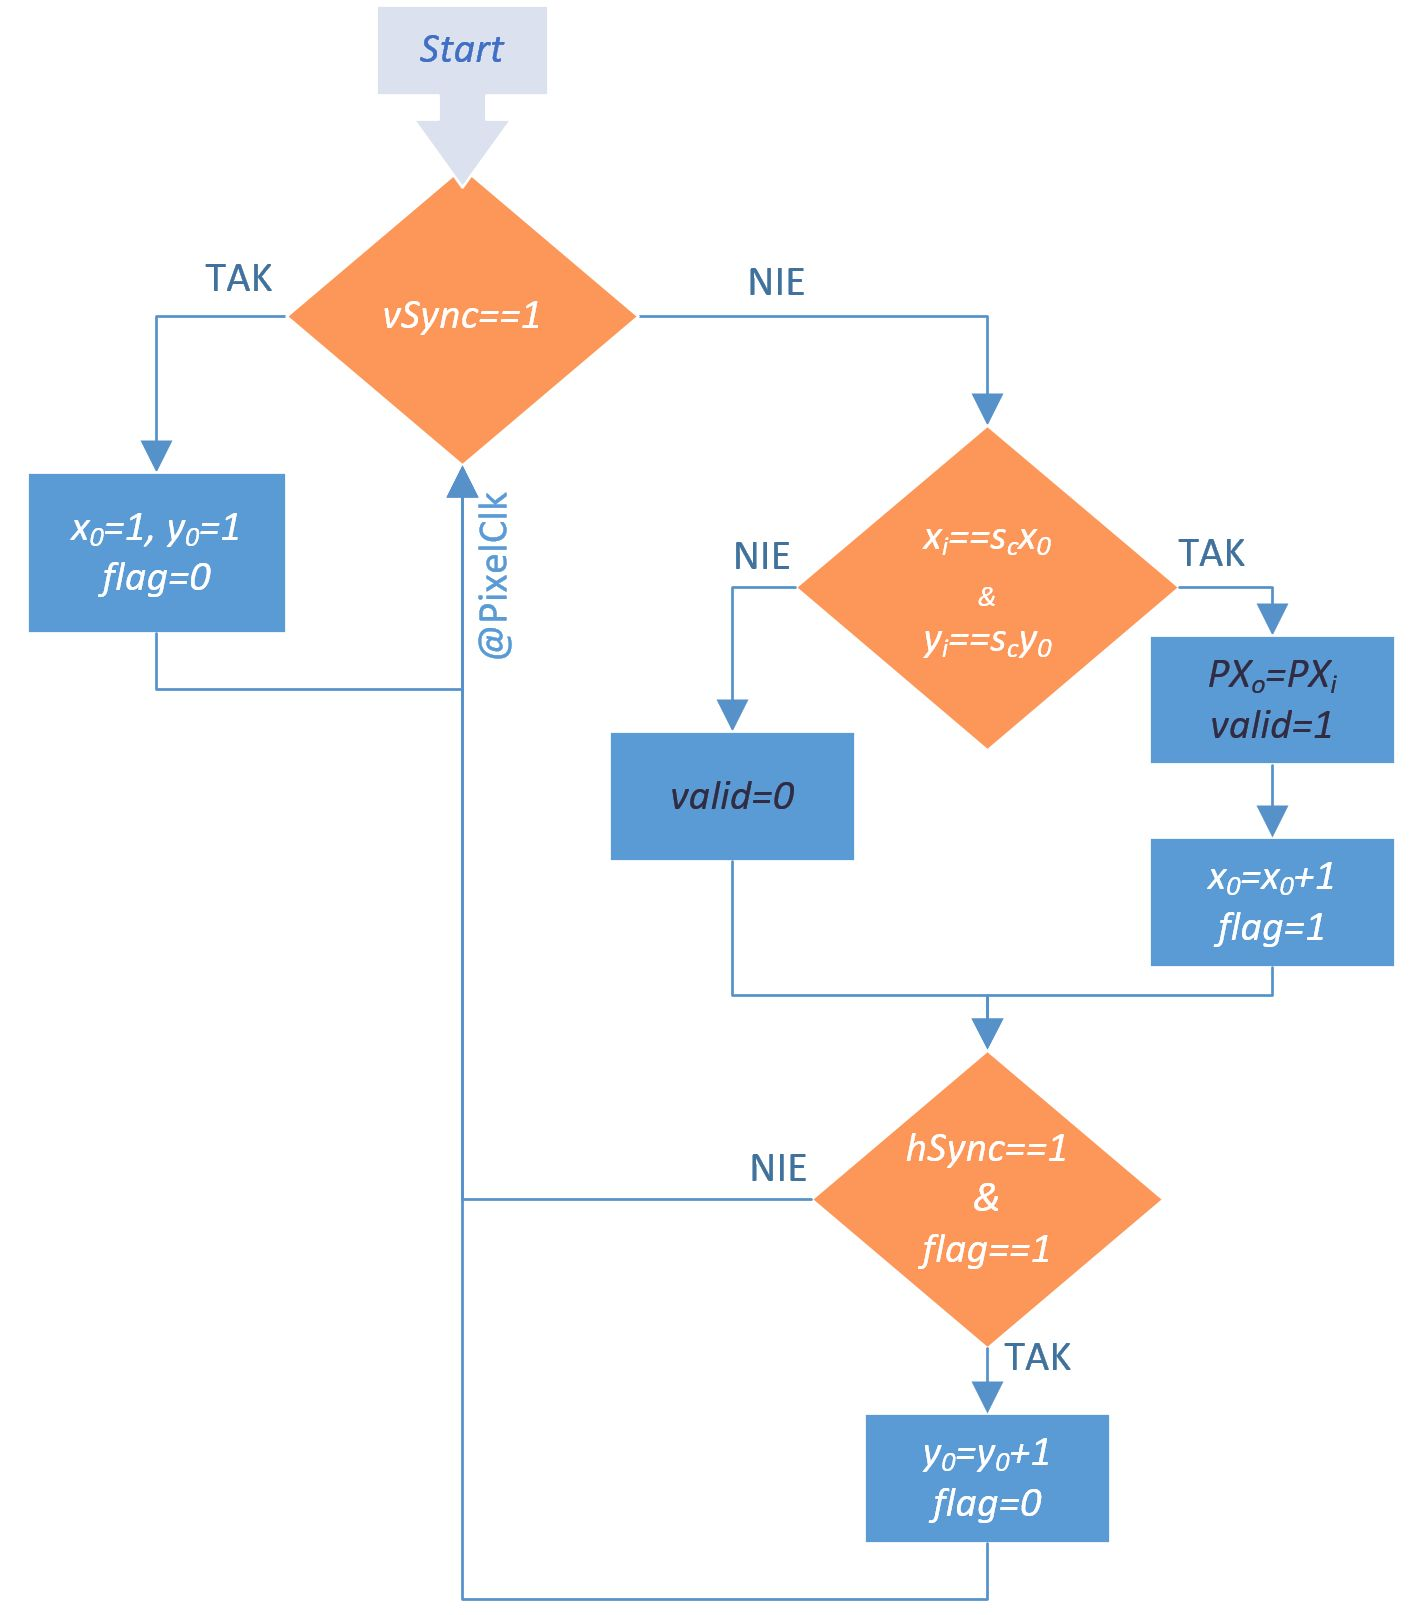
\includegraphics[width=11cm]{4_scaling.jpg}
	\caption{Schemat działania licznika skalującego}
	\label{fig:scaling_sch}
\end{figure}
%TODO jednak opis tego schematu. %ODP dodano nad schematem

Gwarancją poprawnie przeprowadzonego procesu skalowania jest obecność sygnałów sterujących VGA -- tylko wtedy następuje poprawny przyrost wartości liczników. 
Z kolei inicjalizacja (po lewej stronie diagramu) ma miejsce po otrzymaniu sygnału synchronizacji pionowej, zatem podłączony do układu sygnał wideo będzie skalowany już od pierwszej pełnej klatki.

%TODO albo tu albo wcześniej jest potrzebny schemat jak to wygląda - może ogólny. Że jest ramka wejściowa. 5 wynikowych potem HOG i klasyfikacja.

\subsection{Obliczanie gradientów}

Nawet odpowiednio przeskalowane obrazy są zbyt duże, by przechowywać informację o ich gradientach w wewnętrznych zasobach układu XC7Z020. %TODO to zdanie jest niejasne... chyba, żeby je zapamiętać bez wykorzystania zewnętrznej pamięci RAM. %ODP OK
Nie ma jednak takiej potrzeby, jeśli zastosuje się implementację algorytmu z maksymalizacją przetwarzania potokowego, opartego o sygnał aktywnego piksela \textit{valid} z modułu skalowania. %TODO postawi się -> złe sformułwoanie (zastosuje,wykorzysta) %ODP OK

Implementacja gradientu pionowego jest nieco złożona, gdyż wymagane w pojedynczej operacji piksele leżą w kilku kolejnych liniach obrazu. 
Konieczne jest zapamiętanie dwóch ostatnich linii -- zrealizowano to przy użyciu dwóch kolejek FIFO \ref{fig:fifo_gradient}.
Do jednej z nich (oznaczonej numerem \#1) wpisywane są wartości bieżących pikseli.
Przejście do każdej kolejnej linii obrazu powoduje systematyczną wymianę pikseli na najnowsze - wówczas do kolejki \#2 są zapisywane wartości bezpośrednio z \#1. %TODO trochę potoczny styl tego opisu. Najlepiej rysunek (takie jak jest) %ODP nieco poprawiono
Logika została zaprojektowana w sposób pozwalający uzyskać jednoczesny dostęp do 3 kolejnych pikseli leżących w linii pionowej. 
Umożliwia to specjalny tryb modułu FIFO -- First Word Fall Through (FWFT), dzięki któremu pierwsze dostępne słowo jest natychmiastowo wystawiane na wyjście, i tylko zdejmowane (zastępowane kolejnym) w odpowiedzi na wysoki stan sygnału odczytu \cite{FIFO}. %TODO nie duża załuga, tylko umożliwia to %ODP OK
Ostatecznie logika, będąc w linii $i$ ($i>1$), obliczy gradient pionowy dla piksela z linii $i-1$. %TODO nie poniżej tylko \ref. no i nie algorytm %ODP OK, \ref umieszczono wyżej
\begin{figure}[h]
	\centering
	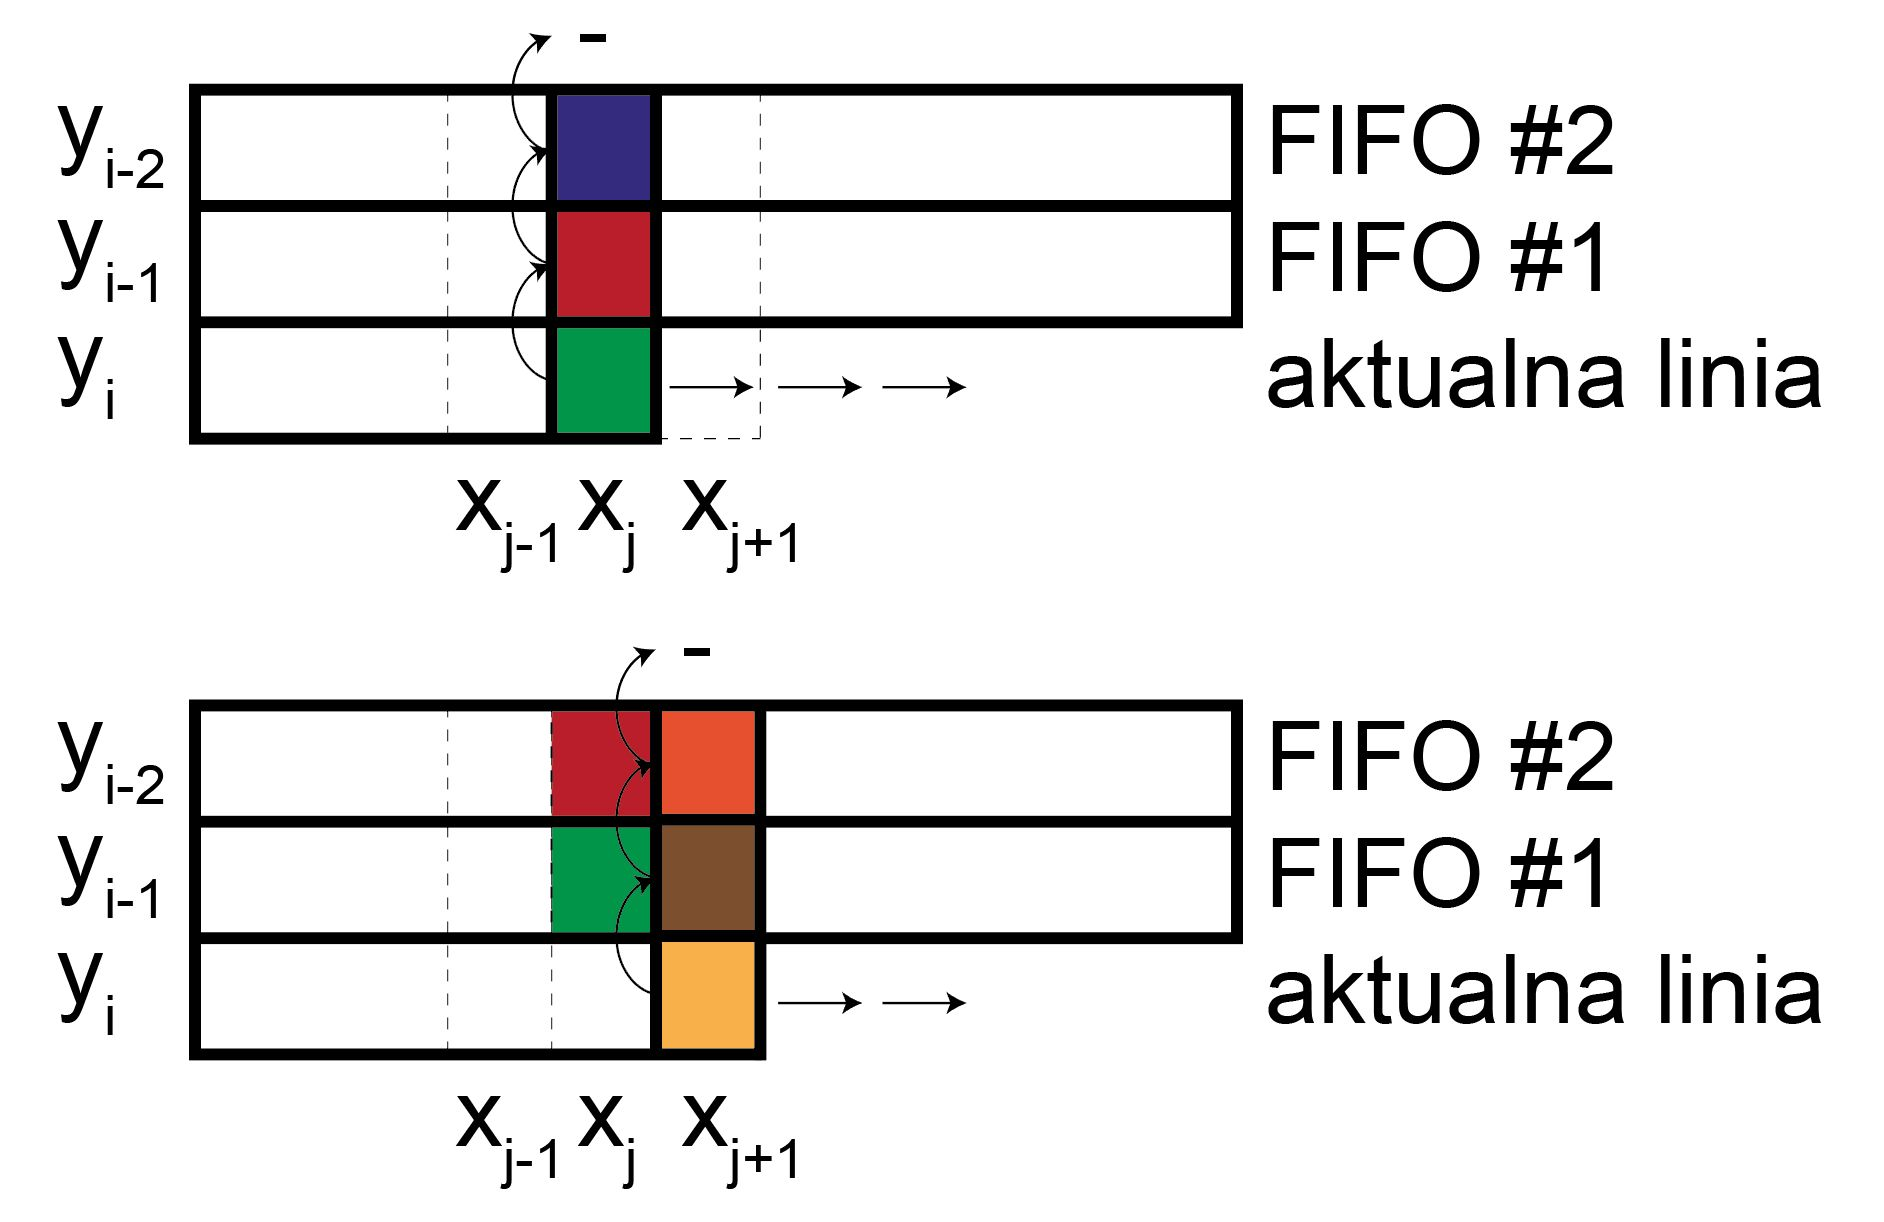
\includegraphics[width=11cm]{4_fifo_gradient.jpg}
	\caption{Schemat działania kolejek FIFO w procesie obliczania gradientu pionowego}
	\label{fig:fifo_gradient}
\end{figure}

Obliczanie gradientu poziomego nie nastręcza już tak wielu trudności -- sąsiadujące ze sobą piksele pojawiają się tuż po sobie, jednak w tym wypadku zamiast aktualnych wykorzystywane są piksele wychodzące z FIFO \#1 i zapamiętywane w rejestrze przesuwnym. 
Oznacza to, że w chwili pojawienia się na wejściu do modułu nowego piksela ($i,j$), obliczony zostanie gradient poziomy piksela ($i-1,j-1$). 
Przez tę latencję potrzebne jest również nieznaczne opóźnienie gradientu pionowego, by obie wartości były zsynchronizowane i ustawione na wyjściu w tym samym momencie.

Sytuacje opisane powyżej dotyczą gradientów dla pikseli wewnątrz obrazu. 
Dla piksela znajdującego się na „początku” obrazu (lewa oraz górna krawędź), gradientem będzie dwukrotność różnicy pomiędzy nim a jedynym jego sąsiadem -- w odpowiedniej osi. %TODO nie na początku tylko na brzegu. Swoja drogą to normalnie się to pomija. %ODP pomija się opis, czy obliczenia gradientów brzegowych?

Poprzednie obliczenia były przeprowadzane w oparciu o sygnał aktywnego piksela ($valid$), którego zbocza były wykorzystywane do określenia gradientów aż do przedostatniego wiersza i kolumny obrazu ($i-1, j-1$). %TODO powt. obliczenia
Piksele znajdujące się przy prawej i dolnej krawędzi ekranu wymagają innego podejścia. 
W tym przypadku, wymagane było stworzenie logiki kontynuującej obliczenia i generującej wyjściowe sygnały aktywne pomimo brak sygnału ($valid$). 
Opisywana sytuacja to również brak nowych wartości pikseli dla kolejek FIFO, co skutkuje ich spodziewanym opróżnieniem krótko po odebraniu pełnej ramki obrazu.
O ile poprzednio tempo obliczania kolejnych gradientów było podyktowane obecnością nowych pikseli, to w tym przypadku logika korzysta wyłącznie z opróżnianych kolejek FIFO, redukując odstęp pomiędzy wynikami do minimum (1 cykl zegara), co jest w zasadzie bez znaczenia dla dalszych obliczeń, które korzystają z poprawnie wygenerowanego sygnału aktywnego sygnalizującego obecność wyniku na wyjściu.


%TODO to jest trochę niejasne %ODP postarałem się nieco uporządkować ten paragraf

\subsection{Histogram gradientów}

Obliczone gradienty stanowią wejście modułu obliczającego wartość $arctg(\frac{g_y}{g_x})$. %TODO a moduł nie ? %ODP OK
Fragment logiki odpowiedzialny za obliczenie modułu został zrealizowany przy użyciu dwóch mnożarek dla obu gradientów, a sumę ich kwadratów następnie poddano pierwiastkowaniu, również w bloku CORDIC. %TODO w bloku - a to opisać wcześniej przy atan %ODP OK
Wykorzystano tutaj blok IP CORDIC \cite{CORDIC}, który na wejściu spodziewa się wektora złożonego z licznika oraz mianownika o tych samych długościach, przy czym jego całkowita długość jest zaokrąglana do wielokrotności liczby 16. 
Gradienty uzyskane z poprzedniego modułu są zapisane w notacji S9.1, zatem wektor wejściowy musi mieć długość 32 -- po 16 bitów na oba gradienty.
Bardziej znaczące bity tych połówek zostały wypełnione zerami i nie mają znaczenia dla obliczeń.
 
Moduł będzie rozpoczynać obliczenia dla danych wejściowych tylko w przypadku, gdy policzone zostały oba gradienty (dwa niezależne sygnały \textit{valid\char`_x/y}) oraz gdy przynajmniej jeden z nich jest różny od zera ($\frac{0}{0}$ jest elementem nieoznaczonym, z którego nie sposób policzyć implementowaną funkcję). 
Opisane warunki \textit{valid\char`_x/y}, połączone odpowiednimi operatorami logicznymi, wyprowadzono jako sygnał aktywny modułu. %TODO potoczne spięte %ODP OK

Otrzymane wartości należy następnie umieścić w dziewięciu 20-stopniowych przedziałach, co opisuje schemat \ref{fig:hog_gradient}. 
\begin{figure}[!ht]
	\centering
	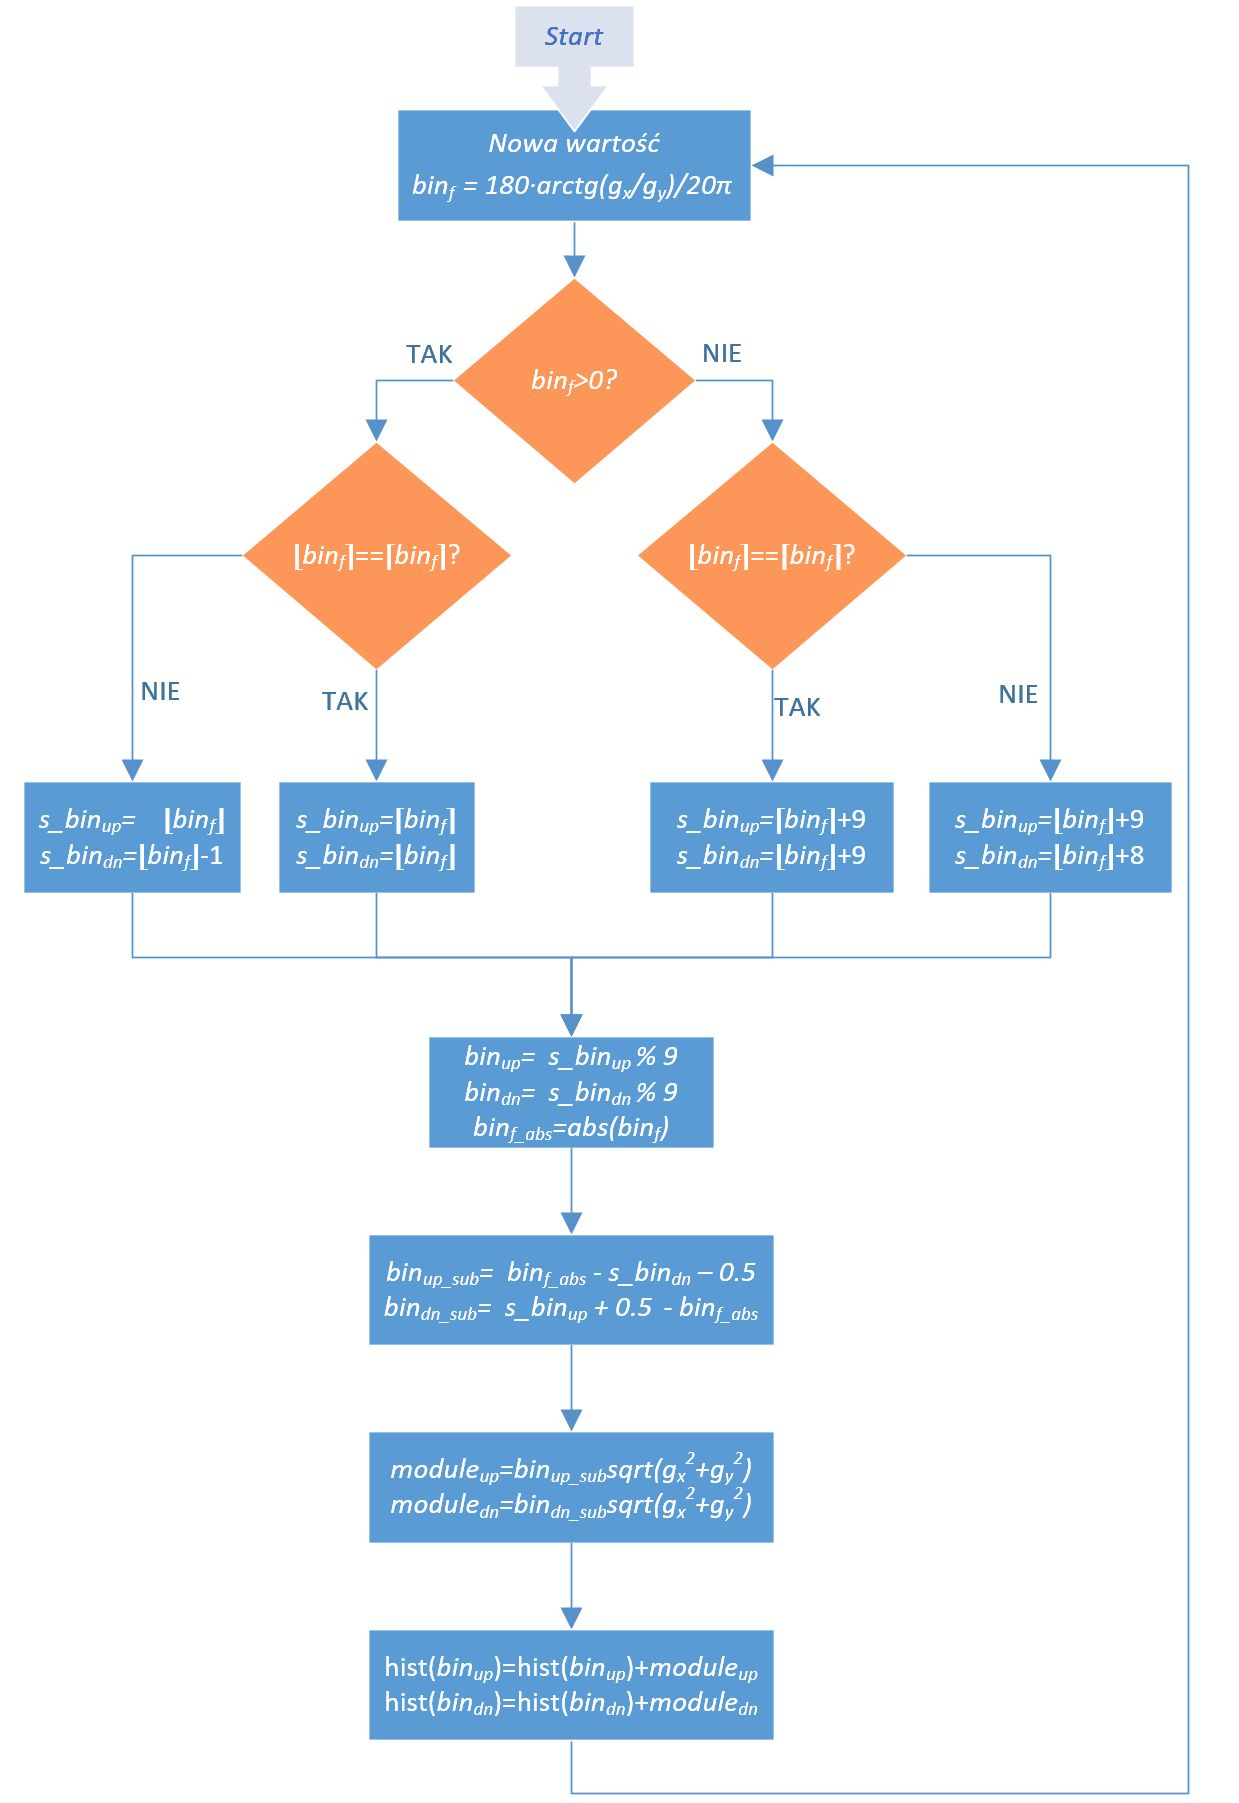
\includegraphics[width=12cm]{4_HOG_gradients.jpg}
	\caption{Schemat działania obliczeń prowadzących do utworzenia histogramu gradientów}
	\label{fig:hog_gradient}
\end{figure}
Pierwszym krokiem jest operacja mnożenia kątów podanych w radianach przez $\frac{180}{20\pi}$, która konwertuje je do liczb ułamkowych stanowiących wstępny przydział (niech będzie to $bin_f$).

Następnie, w zależności od położenia względem środka danego przedziału, wybierane są przedziały: górny i dolny w postaci liczb całkowitych: $s\_bin_{up}$ oraz $s\_bin_{dn}$. 
Ostateczne będą one jednak wymagać normalizacji do postaci liczb z zakresu 0-8 i dopiero wówczas
dwa przedziały histogramu zostaną powiększone o interpolowane wartości modułu gradientów. %TODO coś źle na początku zdania, też ta personifikacja %ODP OK

W procesie obliczania modułu, suma mnożeń podnoszących gradienty do kwadratu jest wektorem U21.2, który poprzez dopisanie bitu '0' rozszerzono do U21.3. 
Zgodnie z dokumentacją bloku CORDIC, wektor o tej długości jest traktowany jako U1.23 -- zatem jest wirtualnie przemnożony przez $2^{20}$. 
Wartość wyjściową należy później interpretować jako U11.13 (wirtualnie podzieloną przez $\sqrt{2^{20}}=2^{10}$). 
Podstawową informacją wykorzystywaną w interpolacji jest odległość $abs(bin_f)$ od środków przedziałów $s\_bin_{up}$ oraz $s\_bin_{dn}$. 
Na tej podstawie obliczane są $module_{up}$ oraz $module_{dn}$ których suma jest równa pełnemu modułowi gradientów.
Ostateczne informacje -- to jest dane o przedziałach i odpowiadające im części modułu zostały przekazane dalej, wraz z wygenerowanymi sygnałami aktywnymi, które sygnalizują obecność wyniku. %TODO co to są wygenerowane sygnały aktywne %ODP OK

Cały powyższy fragment podrozdziału skupiał się na operacjach związanych z pojedynczym pikselem. 
Teraz należy spojrzeć jednak z innej perspektywy, mianowicie na grupowanie pikseli w komórki, bloki i tworzenie wektorów cech na podstawie histogramu. 

Jak opisano we wstępie do rozdziału, najlepszy rezultat detekcji osiągnie się, realizując klasyfikację w obszarze zainteresowań dla jak największej liczby wektorów cech. Te powinny być wygenerowane dla fragmentów obrazu, których przesunięcie względem siebie jest jak najmniejsze -- zilustrowano to na rysunku \ref{fig:HOG_mesh}. %TODO to jest niejasne %ODP OK
Informacje o wektorach cech są zapisywane w pamięci BRAM, %TODO ale jakie ? %ODP OK
jednak szybki przyrost zużycia zasobów układu ogranicza implementację do przetwarzania jedynie określonej liczby obszarów w sąsiedztwie miejsca podejrzewanego o obecność postaci - dane te muszą być przechowane jednocześnie do momentu zakończenia klasyfikacji. %TODO lepiej opisać, bo nie wiadomo dlaczego ten przyrost ma nastąpić. %ODP OK

By nie zużywać cennego miejsca w blokach BRAM, zdecydowano się zapisywać surowe histogramy, a nie gotowe wektory cech -- wiedząc, że dalsza logika dokonując odczytu z tej pamięci, w odpowiedni sposób przekaże te informacje do klasyfikatora. %TODO marnować - potoczne. %ODP OK
Ostatecznie, pojedyncze okno detekcji $128\times 64$ to $32\cdot16=512$ histogramów, czyli $4608$ wartości. 
Wektor cech to aż $31\cdot15\cdot4\cdot9=16740$ wartości. %TODO no właśnie... a dlaczego właściwie użył Pan 4x4 a nie 8x8 - proszę napisać (może przy modelu programowym) %ODP opisano w podrozdziale związanym z uczeniem
Oszczędność wynikająca z zapisu pojedynczych histogramów pozwoli utworzyć znacznie więcej wektorów cech. 
Przykładowo, dla okna o wielkości $144\times 96$ należy zapisać $7776$ wartości. 
Pozwala to jednak wygenerować $9\cdot5=45$ wektorów cech. 
Gdyby zaś wpisywać je do pamięci w gotowej formie, wymagałoby to aż $16740\cdot45=753300$ elementów. %TODO to pozycji to złe słowo %ODP OK

Pamięć RAM należy potraktować jako zbiór 9-elementowych histogramów ułożonych obok siebie. 
Przetwarzanie obrazu, rozumianego jako obiekt dwuwymiarowy, wymaga odpowiedniego mapowania tworzonych wartości do postaci jednowymiarowej, adresowej. 
Schemat \ref{fig:hog_histogram_scheme} przedstawia działanie logiki na ramce obrazu w kontekście zapisu histogramów do pamięci. %TODO styl. sposób pracy %ODP OK
Symbolem „$<=$” określa się przypisanie nieblokujące, które rzeczywisty efekt będzie miało dopiero na następnym zboczu narastającym zegara (i może być zastąpione kolejnym przypisaniem w obrębie jednego cyklu zegara).
 
\begin{figure}[]
	\centering
	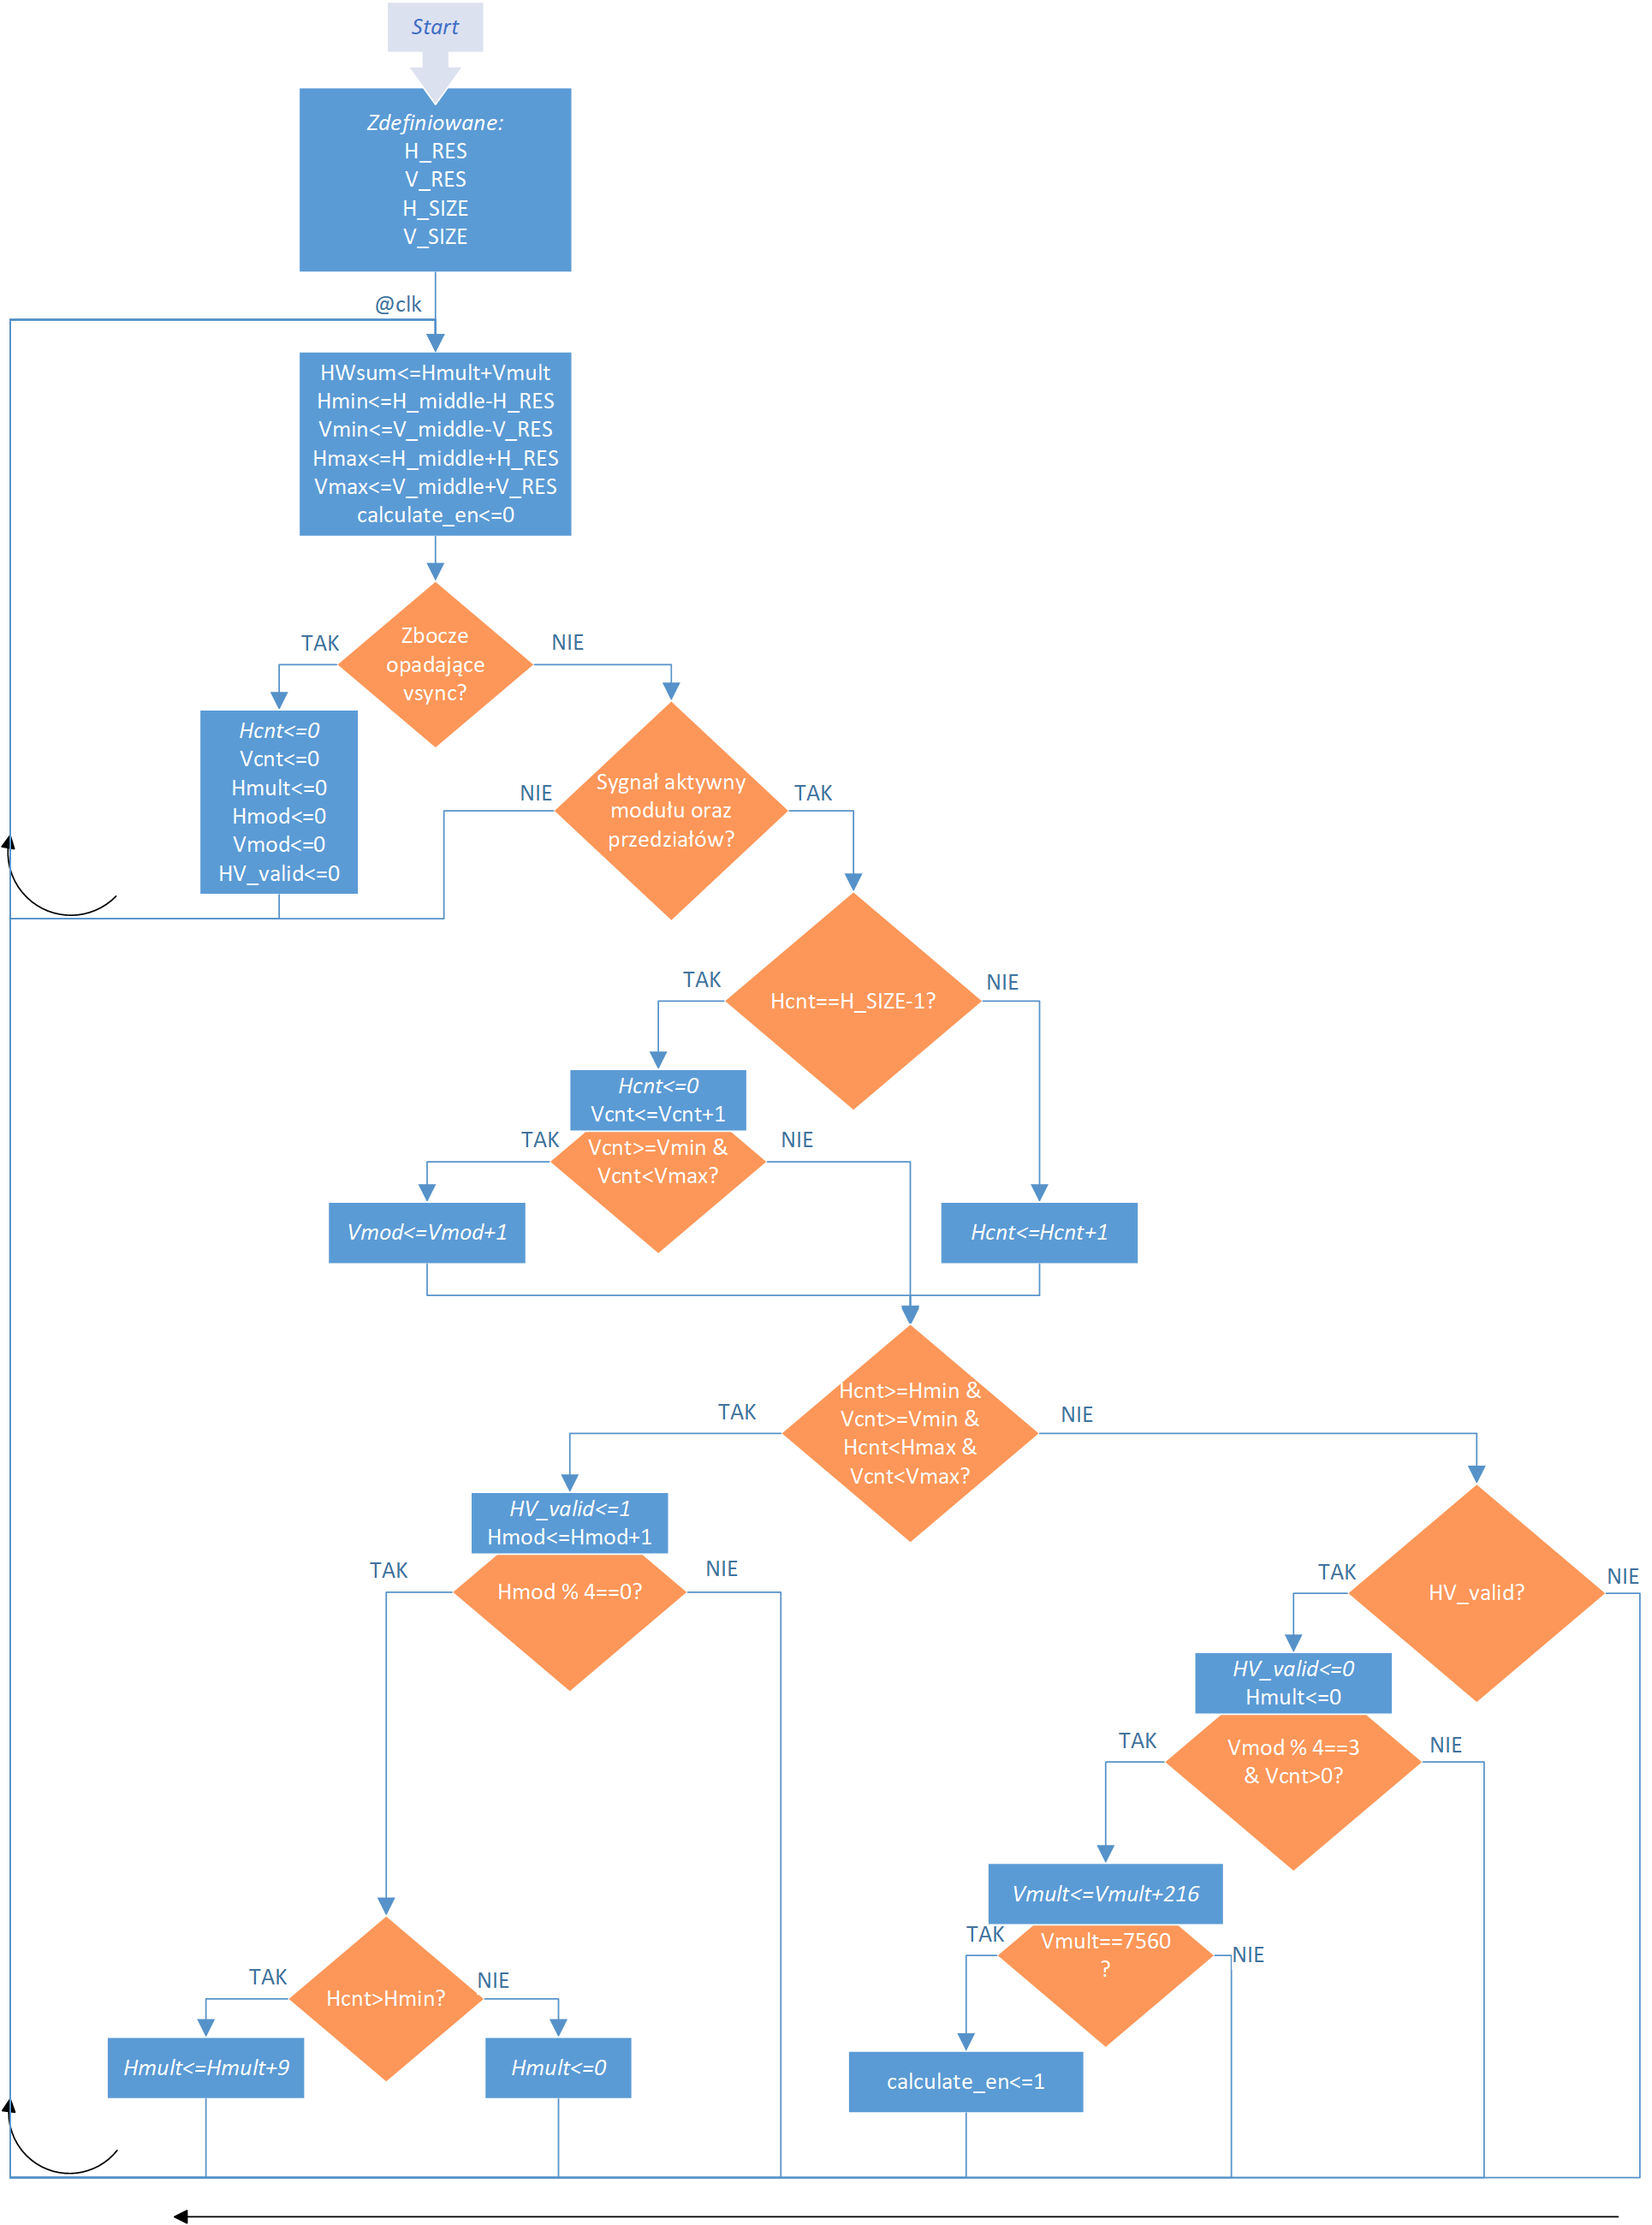
\includegraphics[width=16cm]{4_HOG_Histograms.png}
	\caption{Procedura wyboru adresu pamięci RAM w oparciu o pozycję aktualnego piksela}
	\label{fig:hog_histogram_scheme}
\end{figure} 
%TODO Dlaczego x2 H_RES i V_RES %ODP Poprawiono
%TODO Obawiam się, że ten schemat bez opisu słownego (po tym wymienienu paramtrów) jest nieczytelny (tzn. trudny w odbiorze) %ODP opisano po liście parametrów
 
Określenie aktualnego położenia na obrazie jest możliwe dzięki zastosowaniu liczników, opierających swoje działanie na obecności sygnału aktywnego sygnalizującego gotowe dane wejściowe.
%TODO co to jest ten syg. aktywny %ODP OK
Wykorzystano następujące parametry:
\begin{itemize}
	\item \textit{H\_SIZE}, \textit{V\_SIZE} -- rozdzielczość obrazu przeskalowanego (indywidualnie dla każdej skali),
	\item \textit{H\_middle}, \textit{V\_middle} -- współrzędne piksela środkowego, będącego w centrum analizowanego obszaru (w odniesieniu do odpowiedniej skali, dostarczone przed rozpoczęciem analizy pełnej klatki),
	\item \textit{H\_RES}, \textit{V\_RES} -- wartości określające zasięg analizowanego obszaru -- w odległości od piksela środkowego - dla tego projektu są to odpowiednio: $96/2=48$ oraz $144/2=72$,
\end{itemize}
oraz zmienne:
\begin{itemize}
	\item \textit{Hcnt}, \textit{Vcnt} -- zmienne inkrementowane odpowiednio do wartości maksymalnych \textit{H\_SIZE}, \textit{V\_SIZE} -- pozwalają określić aktualne położenie na obrazie (i względem analizowanego obszaru),
	\item \textit{HV\_valid} -- sygnał aktywny, który wysokim stanem informuje o aktualnym położeniu wewnątrz analizowanego obszaru,
	\item \textit{Hmod}, \textit{Vmod} -- liczniki modulo służące do rozdzielenia pikseli wchodzących w skład różnych histogramów (kwadratów o boku $4\times 4$),
	\item \textit{Hmult}, \textit{Vmult} -- zmienne będące bazą adresową do zapisu aktualnego histogramu (horyzontalna zmienna powiększana o $9$, wertykalna o $9\cdot24$ -- liczba histogramów w linii poziomej),
	\item \textit{calculate\_en} -- sygnalizacja zakończonego procesu obliczania i zapisywania histogramów -- gotowość do rozpoczęcia normalizacji i klasyfikacji dla danej skali. %TODO a gdzie normalizacja ? %ODP normalizacja w module klasyfikacyjnym, więc odbywa się później - ale dla poprawności dodano tu ten termin 
\end{itemize}
Logika, działająca niezależnie dla każdej skali, jest reinicjalizowana po odebraniu sygnału nowej ramki (\textit{vsync}). W momencie otrzymania informacji o kolejnym zestawie przedziałów i modułu, liczniki \textit{Hcnt} oraz \textit{Vcnt} warunkują jego obecność w oczekiwanym obszarze detekcji. Jeśli wynik jest pozytywny, liczniki modulo \textit{Hmod} i \textit{Vmod} są inkrementowane -- odpowiednio co każdy piksel w obszarze, oraz co kolejną linię w obszarze. Podzielność któregokolwiek z nich przez 4 oznacza zmianę histogramu dla kolejnych danych -- wymaga to powiększenia rejestru \textit{Hmult} o 9, lub \textit{Vmult} o 216. 
Ostatecznie, dostępy do odpowiednich adresów pamięci są przedstawione równaniem:
\begin{equation}
\label{eq:adressing_hist}
\left.\begin{aligned} 
addr_{up}&=Hmult+Vmult+s\_bin_{up} \\ 
addr_{dn}&=Hmult+Vmult+s\_bin_{dn}
\end{aligned}\right.
\end{equation}
Pamięć histogramu pracuje w trybie True Dual Port, umożliwiając jednoczesny dostęp do dwóch interpolowanych przedziałów aktualnego histogramu, $s\_bin_{up}$ oraz $s\_bin_{dn}$. 
Zapis danych do pamięci histogramu jest realizowany po odczycie aktualnych wartości komórek i powiększeniu ich o odpowiednie części modułu: $module_{up}$ oraz $module_{dn}$. %TODO Styl. %ODP OK



\subsection{Uczenie}
Założeniem jest, by podczas pracy systemu wbudowanego nie ingerować we współczynniki, a opierać się na pierwotnych wynikach uczenia. %TODO raczej ? %ODP usunięto, niepotrzebny wtręt
Dane te muszą być przechowane w odpowiedni sposób, by możliwy był do nich prosty i szybki dostęp. 
Postanowiono zapisać wektor w pamięci ROM inicjalizowanej plikami \textit{*.mem}, utworzonymi podczas wykonywania skryptu uczenia w MATLABie.
Ręcznie dostosowany moduł pamięci posiada trzy niezależne sektory (w zakresie adresowania i długości danych), inicjalizowane następującymi informacjami: 

\begin{itemize}
	\item składniki skalujące \textit{shifts} -- 16740 elementów wymaganych do przesunięcia każdego elementu wektora cech. Wartości w przedziale: $<-0.2616, -0.0527>$; precyzja zapisu: S0.11.
	\item współczynniki maszyny wektorów nośnych \textit{vectors}. Wartości w przedziale: $<   -0.0076, 0.0063>$; precyzja zapisu: S0.27 (w formacie S0.23, lecz 4 najstarsze bity mają zawsze postać bitu znaku).
\end{itemize}

%TODO nie za bardzo rozumiem te składniki i czynniki %ODP to wsyzstko to współczynniki stanowiące wyjście z funkcji 'svmtrain' MATLABa. Przeanalizowałem w kodzie, jak MATLABowy klasyfikator 'svmclassify' wykorzystuje te dane, i na tym oparłem właściwie swoją logikę.

Dodatkowym współczynnikiem jest wartość przesunięcia gotowego wyniku o precyzji S0.40, jednak jest ona przechowywana w logice. 
Powyższa pamięć zajmuje aż 36 z wszystkich 140 bloków BRAM dostępnych w rozważanym układzie. %TODO dostęþnych w rozważanym układzie %ODP OK
Należy zauważyć, iż wymusza to współdzielenie pojedynczej instancji modułu we wszystkich procesach klasyfikacji. 
Z tego względu istotne jest stworzenie logiki synchronizującej początek przetwarzania wektorów cech ze wszystkich skal -- opisane jest to kolejnym podrozdziale.

\subsection{Klasyfikacja}


Po obliczeniu wektorów cech następuje proces klasyfikacji %TODO gdzie podziała się normalizacja w blokach ???%ODP dopisano, opis po schemacie
Poprzedza ją normalizacja w blokach, która jest częścią tego modułu ze względu na obecność każdego histogramu w kilku różnych blokach. 
Odczytywane z pamięci ROM wartości współczynników klasyfikatora muszą być współdzielone pomiędzy obliczeniami przeprowadzanymi dla każdej ze skal obrazu, jednak w każdym przypadku tempo generowania histogramów nie jest jednakowe -- proces ten przebiegnie szybciej dla większych obrazów (tam analizowany fragment obrazu pojawi się na wejściu wcześniej). 
O gotowości histogramów z odpowiedniej skali informuje indywidualny dla niej sygnał \textit{calculate\_en}. 
Dopiero w momencie otrzymania wszystkich sygnałów \textit{calculate\_en} (stan wysoki na wyjściu iloczynu logicznego) rozpoczynany jest właściwy proces klasyfikacji.

Moduł odpowiadający za sklasyfikowanie informacji pochodzących z pojedynczej skali zrealizowano w formie krótkiej maszyny stanu, na którą składają się następujące etapy:
\begin{itemize}
	\item inicjalizacja -- oczekiwanie na sygnał \textit{full\_frame}, informujący o rozpoczęciu algorytmu na pełnej klatce obrazu
	\item czyszczenie pamięci przechowującej wektory cech z poprzednich uruchomień algorytmu -- etap ten ma miejsce tuż po otrzymaniu sygnału \textit{full\_frame}, który pojawia się podczas stanu wysokiego synchronizacji pionowej; jest wykonywany na tyle szybko, by pamięć mogła być bezpiecznie zapisana wartościami histogramów z nowej ramki obrazu %TODO zdącyż - potoczne. Ale to chodzi o tą pamięć histogramów ??? %ODP tak, niezbyt dobre miejsce na akurat ten element logiki, mogło być gdzieś bardziej na topie... ale już szkoda ryzykować ew. błędy.
	\item oczekiwanie na iloczyn sygnałów \textit{calculate\_en}; inicjalizacja zmiennych algorytmu
	\item właściwa normalizacja i klasyfikacja
\end{itemize}

O ile zapisane w pamięci ROM współczynniki mają postać wektora cech, tak pamięć RAM przechowuje nieuporządkowane fragmenty histogramów. 
Wymagało to stworzenia logiki, która łączy ze sobą dane ze ściśle określonych adresów pamięci, interpretując je w postać deskryptora.  
Opisuje to diagram \ref{fig:hog_feature_histrogram_address}. %TODO nie poniższy, styl.: dane z odpowiendich... %ODP OK

\begin{figure}[h!]
	\centering
	\captionsetup{justification=centering,margin=1cm}
	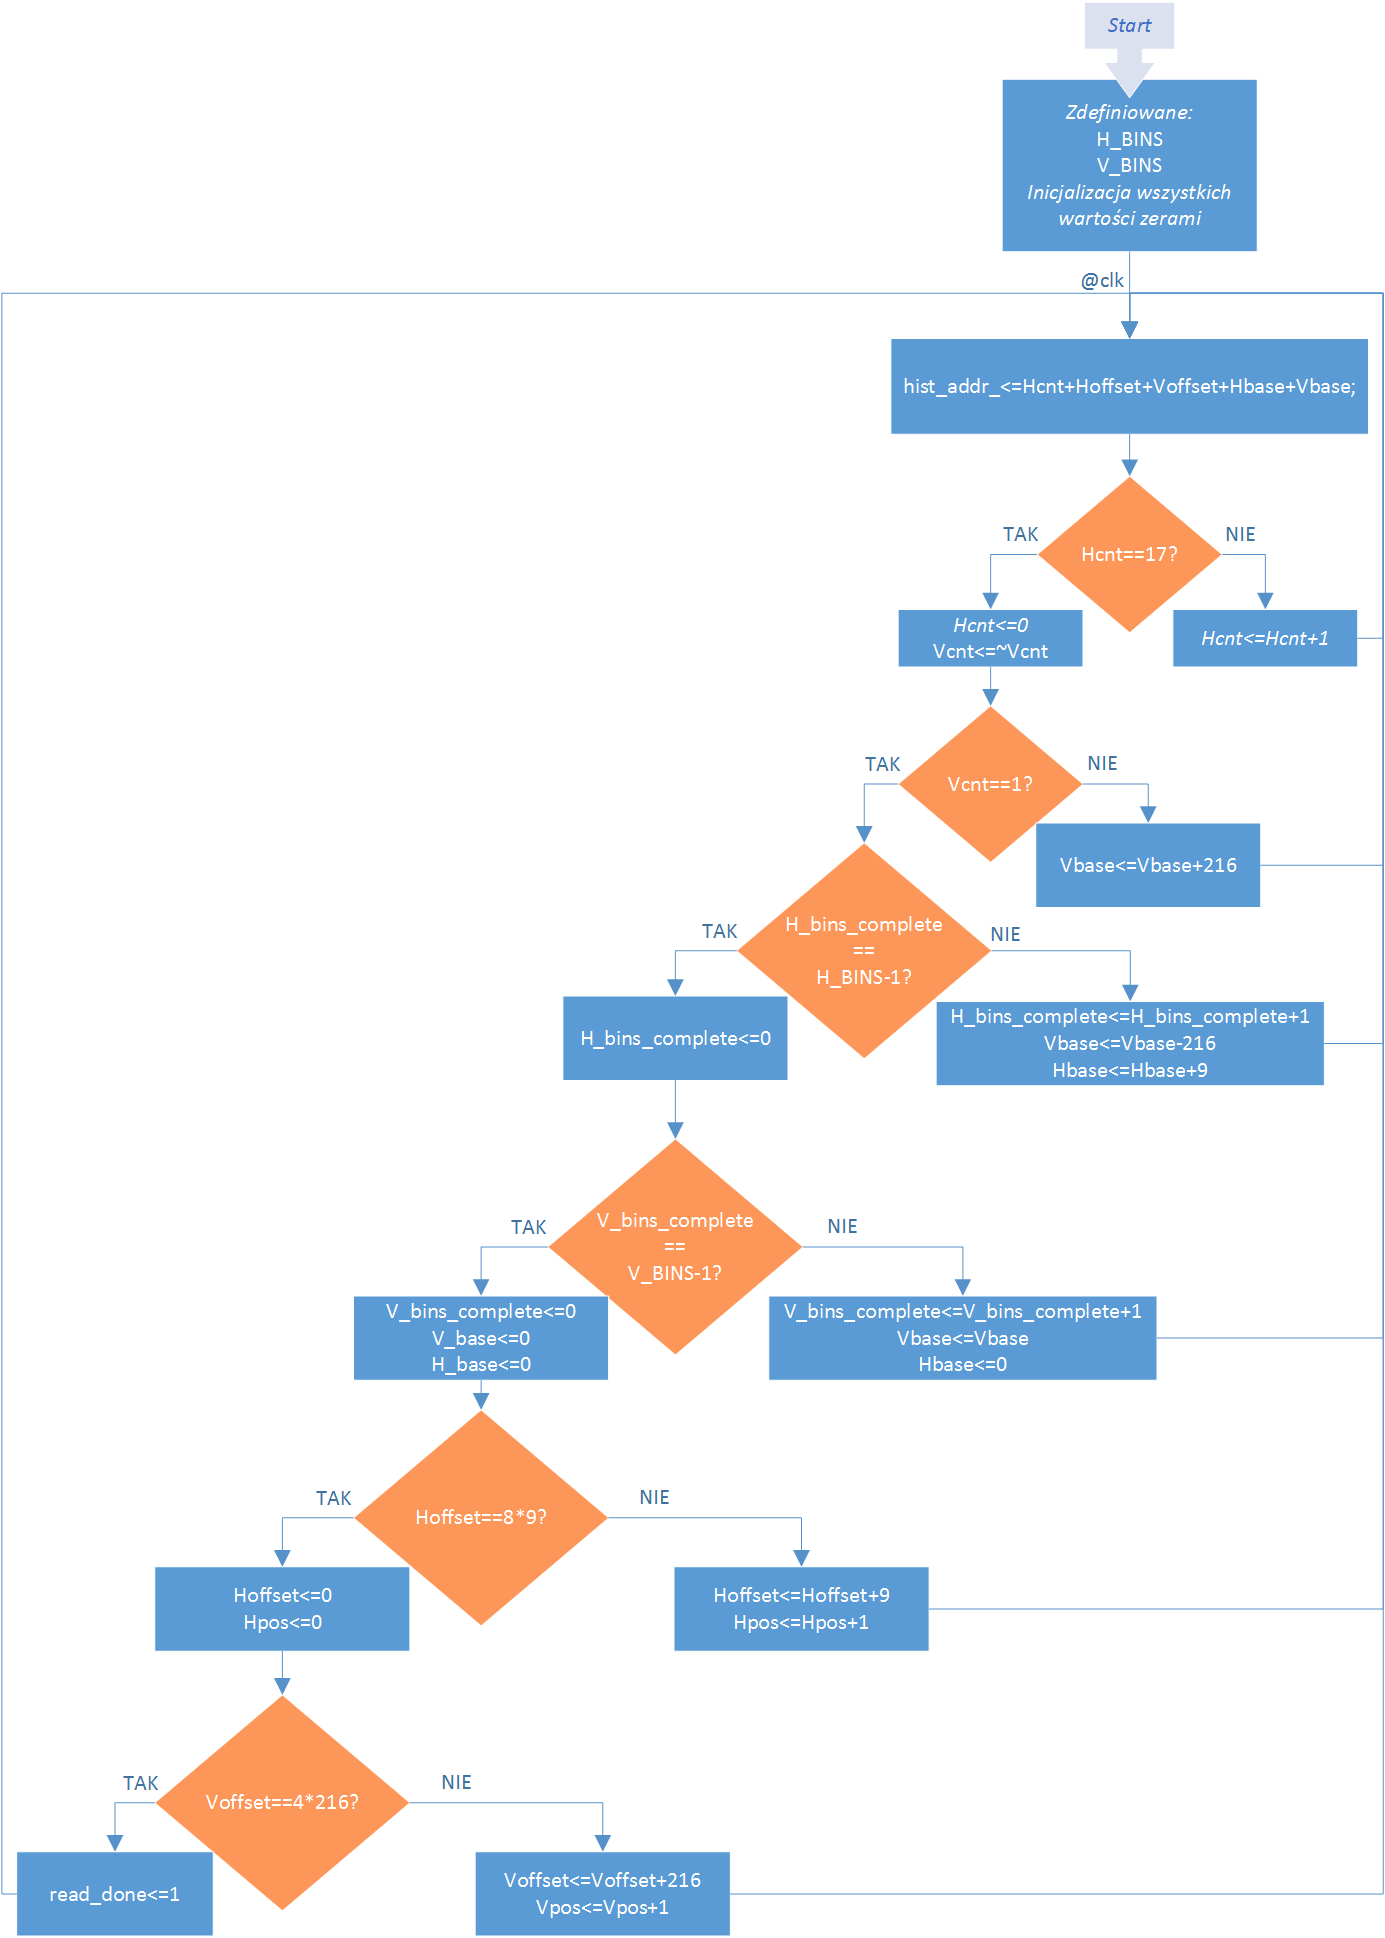
\includegraphics[width=15cm]{4_HOG_Features.png}
	\caption{Procedura wyboru adresu pamięci RAM w procesie odczytu kolejnych histogramów}
	\label{fig:hog_feature_histrogram_address}
\end{figure} 

Kolejnym etapem jest normalizacja w blokach, która ze względu na prostszą realizację została umieszczona wewnątrz procesu klasyfikacji (tym bardziej, że idea bloków właściwie nie funkcjonowała we wcześniejszych modułach). %TODO w blokach, nie bloków %ODP OK
Blokiem jest struktura 4 histogramów, czyli łącznie 36 wartości. 
Odczytane z pamięci RAM dane są podnoszone do kwadratu przez mnożarkę, a następnie sumowane z kolejnymi wynikami. %TODO a nie sumowane %ODP OK, inkrementacja następuje po sumie 36 wartości
Suma 36 takich wartości, dodatkowo zinkrementowana, jest poddawana pierwiastkowaniu i będzie stanowić mianownik w procesie normalizacji powiązanego bloku (zgodnie z równaniem \eqref{eq:HOG_norm3}). 
Moduł pierwiastkujący działa potokowo, więc zwraca również wartość pierwiastkową z niepełnych sum -- dlatego ważne jest wygenerowanie sygnału aktywnego w momencie zsumowania 36 elementów, a także zatrzaśnięcie poprawnej wartości pierwiastka na czas 36 dzieleń.

Normalizacja wymusza ponowne przejście przez odpowiednie dane z pamięci RAM. 
Zastosowanie dwuportowego modułu pozwala na uzyskanie dostępu do uprzednio przetworzonych danych na drugim porcie, podczas gdy pierwszy kontynuuje zwracanie informacji potrzebnych do obliczenia współczynników normalizacji dla kolejnych bloków. %TODO kanale-> porcie %ODP OK
Poprawną kolejność danych na drugim porcie osiągnięto przez odpowiednie opóźnienie sygnału adresowego z portu pierwszego. 

Napływające potokowo dane z portu drugiego, podzielone przez odpowiedni współczynnik normalizacji, mają ustawioną flagę \textit{normalized\_valid}.
Jej stan wysoki rozpoczyna inkrementację adresu pamięci ROM przechowującej współczynniki przesunięć (\textit{shifts}) pochodzące z procesu uczenia. %TODO nie rozumiem shifts. %ODP offset ze struktury klasyfikatora w matlabie
%TODO poza tym. nachodznie bloków na siebie powoduje, że danych jest więcej niż histogramów wejściowych %ODP zgodnie ze zdaniem nieco wyżej: Szybkie obliczenia pokazują, że dla obrazu o wymiarach $128\times 64$ powstanie $32\times 16$ komórek, a idąc dalej, $31\times 15$ bloków po 4 histogramy po 9 wartości, czyli długość wektora cech będzie wynosić 16740. 
Każda z 16740 par zostanie do siebie dodana. 
Znormalizowane elementy wektora cech mają postać U11.13, zatem należało uprzednio rozszerzyć wektor \textit{shifts} do tego formatu. 

Kolejnym krokiem jest wymnożenie każdej z sum przez właściwy współczynnik maszyny wektorów nośnych. %TODO skąd ten czynnik skalujacy ? połączyłem czynnik skalujący ze struktury matlabowskiej z dalszymi czynnikami, teraz mam dwa zestawy danych - 16740 offsetów i 16740 współczynników.
Aby to osiągnąć, należało ponownie i odpowiednio opóźnić linie adresowe uzyskujące dostęp do przestrzeni adresowej danych oraz \textit{vectors}. 
Ostateczna szerokość pojedycznego elementu wynosi S7.40.

Docelowa wartość definiująca detekcję jest sumą wszystkich 16740 przetworzonych elementów oraz jeszcze jednej stałej wyznaczonej na etapie uczenia, \textit{offset} równej $-0.6327$. 
\textit{Offset} stanowi wartość początkową sumy przy rozpoczęciu obliczeń dla kolejnego wektora cech. %TODO dla kolejnego %ODP OK
Ze względu na konieczność zapewnienia dobrej dokładności w procesie sumowania, wynik jest zapisywany w notacji S7.40.

\subsection{Przetwarzanie wyników}

Niezależnie od liczby przetwarzanych skal obrazu, etap klasyfikacji jest dla nich realizowany równolegle, przetwarzając po $5\times 9$ wektorów cech i zakończy się w tym samym momencie. Zarówno tworzenie deskryptorów, jak i klasyfikacja są zaimplementowane w modułach działających w oparciu o zegar $148.5$MHz. Pozwala to zrealizować sam etap klasyfikacji w czasie ok. $5$ms.
Kolejnym etapem jest analiza wyników ze wszystkich skal.
%TODO proszę to jaśniej opisać. Bo to jest tak, że "po kolei" dla każdej ze skal ? i z jakim zegarem ? To jest niejasne. %ODP OK
Jest on dość prosty, gdyż zakłada jedynie porównanie najlepszych rezultatów -- w modułach klasyfikacji każdej ze skal zaimplementowano logikę, która zapamiętuje swoje lokalne minima i parametry obszarów (w odpowiednich skalach), na podstawie których je osiągnięto. 
Skutkiem porównań jest wyłonienie skali z najlepszym wynikiem, a koordynaty tego obszaru zostają dostosowane do rozdzielczości $1280 \times 720$ i mogą być wykorzystane przez warstwę wyższą. %TODO natywnej (średnie słowo) %ODP OK

%TODO Ogólnie - nieco lepszy opis, szczególnie na ogólnym poziomie. I coś z tą normalizacją jest nie tak. %ODP normalizację wyjaśniłem wyżej, poprawiono


%TODO Kolejna sprawa to również jakiś schemat blokowy modułu sprzętowego.

%TODO Dalej. Zużycie zasobów przez moduł mean-shift i hog/svm - tabelki.%ODP OK

\section{Integracja układu FPGA z dronem}

Opisana w poprzednim podrozdziałach architektura sprzętowa dotyczyła dwóch algorytmów, które mogą funkcjonować niezależnie od siebie. Ostnieje jednak jeszcze najwyższa warstwa logiczna, która łączy ich działanie, zwiększając niezawodność działania systemu. Na podstawie ostatecznych wyników śledzenia podejmowane są decyzje związane z ruchem drona. Muszą być one przekazane niezależnej jednostce odpowiedzialnej za stabilizację drona -- autopilotowi. Wymagało do m.in. określenia sposobu komunikacji pomiędzy nim a układem Zynq.
%TODO do rozbudowy, ale w kontekście zawartości 'nowego" rozdziału początkowego. %ODP OK, rozbudowano rozdział początkowy.


\subsection{Zdalne uruchomienie pracy systemu}

%TODO To już może być treść tego rozdziału. Tylko oczywiście po jakimś wstępie. %ODP OK

Początkowo stworzono (i ostatecznie pozostawiono) możliwość rozpoczęcia pracy z wykorzystaniem jednego z przełączników na płycie PYNQ, gdyż prace nad projektem wymagały dość częstego uruchamiania algorytmu jeszcze bez udziału drona. 
Jednak lot maszyny lub nawet jego start praktycznie wyklucza fizyczny dostęp do układu FPGA, dlatego koniecznością stało się zdalne wyzwolenie pracy algorytmów. 
Sygnał wyzwalający nosi nazwę \textit{trigger\char`_algorithm}.

Podczas lotu maszyny użytkownik ma pod ręką jedynie aparaturę radiową, z poziomu której może jednak w dość prosty sposób wysyłać sygnały . %TODO wystawiać - potoczne %ODP OK
Aparatura jest bowiem wyposażona w szereg konfigurowalnych przełączników analogowych i cyfrowych. 
Ponadto, dane są wysyłane poprzez 16 kanałów -- przy czym do kontroli podstawowych funkcji drona wykorzystuje się zaledwie 4. %TODO raczej nie 16 kanałów tylko przez / poprzez... %ODP OK
Wybrano zatem jeden z pozostałych dostępnych kanałów, któremu przypisano funkcję trzypoziomowego przełącznika obecnego na panelu urządzenia radiowego.

Sparowany z aparaturą odbiornik, który jest zamocowany na dronie, wysyła wszystkie dane po jednym zestawie przewodów w formie PPM (ang. \textit{Pulse Position Modulation}). %TODO napisać, że odbiornik jest na dronie %ODP OK
Taki sygnał musiałby być zdekodowany w części PL układu Zynq do uzyskania użytecznej wartości. %TODO nie nie FPGA.. Zynq/lb PL %ODP OK
Proces dekodowania rozwiązuje jednak autopilot, który konwertuje 16-kanałowy PPM na znacznie prostsze sygnały PWM (ang. \textit{Pulse Width Modulation}) m.in. do kontroli silników. %TODO wystawia %ODP OK
Co więcej, Pixhawk umożliwia przypisanie reszty kanałów transmisyjnych do pomocniczych wyjść PWM. 
Rozwiązanie to znalazło zastosowanie chociażby w ustawieniu wartości zadanych serwomechanizmom odpowiedzialnym za pracę gimbala kamery.

%Ostatecznie, postanowiono ustalić warunki kwestią niejasną pozostała szerokość pulsu, który miałby wyzwolić działanie algorytmu. %TODO dalczego niejasną ? %ODP rozpisano się na ten temat poniżej
Za pomocą oprogramowania Mission Planner, służącego do konfiguracji autopilota, ustawiono zakres szerokości wysyłanego pulsu PWM na $1100-1900$us. Wybranie odpowiedniej wartości wyzwalającej pracę systemu wymagało dodatkowej weryfikacji, podczas której sprawdzono przypadek z wyłączoną aparaturą radiową (brak wejściowego sygnału PPM) i ewentualne błędy w transmisji PWM.
Do pomiarów zastosowano analizator logiczny ILA wbudowany w środowisko Vivado i stworzono prosty licznik, który jest poddawany następującym operacjom:
%TODO na którym - styl i po co to ILA - do pomiarów. %ODP OK
\begin{itemize}
	\item kasowanie na zboczu narastającym sygnału wejściowego,
	\item inkrementację podczas aktywnego stanu sygnału,
	\item przypisanie tej samej wartości w każdym innym przypadku.
\end{itemize}

Logika jest taktowana zegarem \textit{calc\char`_clk} $=100$MHz i dla poszczególnych pozycji przełącznika na aparaturze radiowej wartości licznika są przedstawione w tabeli \ref{tab:RFswitch}. %TODO do tabeli \ref{HSV_first}, "logika pracuje" styl %ODP OK
Pokazuje ona, że zakres długości pulsu nie odstaje od normy typowego sygnału PWM, mimo że jest nieco zawężony.

\newcolumntype{P}[1]{>{\centering\arraybackslash}p{#1}}
\begin{table}[h]
	\centering
	\caption{Szerokości pulsu PWM dla przełącznika odpowiedzialnego za start algorytmu}	
	\begin{tabular}{|P{3cm} |P{2cm} |P{2cm}|}
		
		\hline
		\rowcolor{lightgray} Pozycja przełącznika & Wartość licznika & Długość pulsu [ms]  \\ 
		-1	& 109000 & 1.09	\\ 
		\hline
		0	& 149000 & 1.49 \\ 
		\hline
		1	& 189000 & 1.89 \\ 
		\hline
	\end{tabular}
	\label{tab:RFswitch}
\end{table}

Na tej podstawie określono, że warunkiem koniecznym do rozpoczęcia algorytmu będzie wystąpienie dwóch kolejnych pulsów o szerokości przynajmniej 1.8ms (górny limit przezornie ustawiono na 2ms). 
Analogicznie, zakończenie pracy algorytmu i powrót do ustawień domyślnych będzie miał miejsce po zmianie pozycji przełącznika z „1”, czyli po otrzymaniu dwóch kolejnych pulsów o szerokościach spoza zakresu $[1.8$ms,$2$ms$]$.
%TODO nie do końca rozumiem jak to z poza zakresu %ODP dopisano dodatkowe info

\subsection{Kontrola pracy algorytmów MeanShift oraz HOG+SVM} %TODO nad pracę -> pracy %ODP OK
Najwyższa warstwa w części programowalnej Zynq jest odpowiedzialna za integrację działania algorytmów MeanShift i HOG+SVM i zarządza sygnałami używanymi do ich niezależnego uruchamiania. %TODO FPGA-> Zynq (to rozumiem, że używa Pan PS w ogóle) i styl do poprawy. %ODP OK, PS używany, minimalnie opisany niżej
\subsubsection{Komunikacja pomiędzy PL i PS}
Nie jest to jednak najwyższy poziom zarządzania -- warstwa ta komunikuje się bowiem z aplikacją uruchomioną w części PS, która jest odpowiedzialna za nadzór nad pracą zarówno autopilota, jak i opisywanej części do tej pory PL układu Zynq.
Komunikacja pomiędzy PS a PL jest realizowana dwutorowo:
\begin{itemize}
	\item PL odbiera ustawienia konfiguracyjne z przestrzeni adresowej 32-bitowych rejestrów. Używanych jest 5 rejestrów, które są inicjalizowane w PS wartościami domyślnymi. Ich opis przedstawia tabela \ref{tab:registersIN}	
	\item PL wysyła informacje 32-bitowym sygnałem GPIO, który jest skonfigurowany w części PS do wywoływania przerwań po każdej jego zmianie. Utworzone są również 2 dodatkowe rejestry, z których dane odczytywane są w PS podczas obsługi tego przerwania. Strukturę przedstawia tabela \ref {tab:registersOUT}
\end{itemize} 

\newcolumntype{P}[1]{>{\centering\arraybackslash}p{#1}}
\begin{table}[h]
	\centering
	\caption{Informacje wysyłane do PS w postaci rejestrów}	
	\begin{tabular}{|P{1.4cm} |p{9.5cm}| p{1.25cm}| p{1.75cm}|}
		
		\hline
		\rowcolor{lightgray} Adres rejestru & Sygnały & Format & Pozycja w rejestrze  \\ 
	    --\newline (GPIO)	& \textit{PL\_to\_PS\_control} -- wymuszenie ruchu drona w oparciu o dane rejestru 0x04\newline
	    \textit{PL\_to\_PS\_status} -- status pracy algorytmów MS/HOG+SVM\newline
		\textit{trigger\char`_algorithm} -- rozpoczęcie misji (sygnał z aparatury radiowej) & 
		U1.0  \newline\newline
		U4.0 \newline\newline
		U1.0  & [12:12]\newline\newline[7:4]\newline\newline[0:0]\\ 
		\hline
		0x04	& $y_{pos}$ -- odegłość do punktu zadanego na osi x obrazu\newline
		$x_{pos}$ -- odległość do punktu zadanego na osi y obrazu\newline
		$z_{scale}$-- wartość skali dla ostatnich detekcji & 
		S10.0  \newline
		S10.0 \newline
		U3.2  & [30:20]\newline[18:8]\newline[4:0] \\ 
		\hline

	\end{tabular}
	\label{tab:registersOUT}
\end{table}

\newcolumntype{P}[1]{>{\centering\arraybackslash}p{#1}}
\begin{table}[h]
	\centering
	\caption{Informacje odbierane z PS w postaci rejestrów}	
	\begin{tabular}{|P{2cm} |p{8cm}| P{1.5cm}| P{2cm}|}
		
		\hline
		\rowcolor{lightgray} Adres rejestru & Sygnał & Format & Wartość domyślna   \\ 
		0x00	& \textit{PS\_to\_PL\_run\_alg} -- kontrola pracy maszyny stanów w PL nadzorującej algorytmy MS/HOG+SVM: \newline0 - nieaktywna\newline1 - aktywna & U1.0& $0$\\ 
		\hline
		0x04	& \textit{SVM\_threshold} -- wartość progu & S7.24 &$-0.1$\\ 
		\hline
		0x08	& \textit{SVM\_strong\_threshold} -- wartość progu drugiego stopnia & S7.24 &$-1$\\ 
		\hline
		0x0C	& \textit{SVM\_lost\_iter} -- maksymalna ilość iteracji opartych wyłącznie na wyniku MeanShift & U15.0 & $100$\\ 
		\hline
		0x10	& \textit{SVM\_iter\_between\_control} -- ilość iteracji algorytmu SVM pomiędzy aktualizacjami uchybu regulacji do PS & U6.0 & $15$\\ 
		\hline
	\end{tabular}
	\label{tab:registersIN}
\end{table}

Do rozpoczęcia pracy algorytmów wymagane jest otrzymanie informacji o gotowości drona, czyli ustabilizowaniu pozycji w powietrzu. Służy do tego rejestr \textit{PS\_to\_PL\_run\_alg} opisany w tabeli \ref{tab:registersIN}


%Zanim jednak przyjdzie na to pora, zadaniem maszyny stanu jest oczekiwanie na informację o gotowości drona, tj. ustabilizowaniu pozycji w powietrzu. %TODO styl. "zbyt powieściowy" %ODP OK

%TODO napisać co wysyła %ODP wyżej opisano całą komunikację PS-PL
\subsubsection{Pierwsza detekcja osoby}
Po otrzymaniu takiego sygnału kolejnym etapem jest skanowanie obrazu w celu pierwszej detekcji postaci. %TODO co znaczy pierwotna %ODP OK
Przy założeniu, że osoba nie pojawi się w górnej i dolnej części ramki obrazu, można ograniczyć obszar poszukiwań do jej środkowego pasa. Wykorzystywany w tym celu algorytm HOG+SVM uruchamiany jest cyklicznie na sąsiednich oknach detekcji w obrębie tego pasa. Przedstawia to ilustracja \ref{fig:scan_scheme}. %TODO na przesuwanym - styl i niejasne. Tak samo to pokryć. %ODP OK
Każda ze skal dysponuje obszarem detekcji o wymiarze $144\times 96$, z którego wybierane jest okno detekcji  $128\times 64$ o najniższej wartości odpowiedzi. %TODO nie najlepszy fragment, tylko okno detekcji o najwyżej wartości odpowiedzi. %ODP OK, tyle że u mnie musi być jak najniższa

Chcąc zapewnić wysoką dokładność detekcji, należy uwzględnić wielkość obszarów dla poszczególnych skal w odniesieniu do oryginalnego obrazu. Okazuje się, że najmniejszą powierzchnię ma obszar związany z najmniejszym współczynnikiem skali - na jego podstawie należy więc oprzeć przesunięcia obszaru poszukiwań. Porównanie skal przedstawia tabela \ref{tab:scale_window_cover}. %TODO też niejsane + \ref do tabeli

Ponadto, analizując działanie algorytmu w pojedynczej skali, dla obszarów o rozmiarach $128\times 64$ oraz $144\times 96$  wyczerpującej analizie poddawanych jest jednorazowo jedynie $20\times 36$ pikseli. By przeanalizować wszystkie okna detekcji $128\times 64$, konieczne jest współdzielenie obszarów pikseli pomiędzy kolejnymi iteracjami algorytmu HOG+SVM. %TODO tego nie rozumiem %ODP opisano nieco więcej 
%TODO może po prostu rysunek schematyczny do tego by wszystko dobrze wyjaśnił %ODP Średnio wiem, jak się tego podjąć żeby z miejsca tłumaczyło czemu jest tak a nie inaczej;)

\newcolumntype{P}[1]{>{\centering\arraybackslash}p{#1}}
\begin{table}[h]
	\centering
	\captionsetup{justification=centering,margin=1cm}
	\caption{Wielkość analizowanego obszaru HOG+SVM dla poszczególnych skal, w odniesieniu do oryginalnej wielkości obrazu}	
	\begin{tabular}{|p{1cm} |P{4cm}| P{5cm}|}
		
		\hline
		\rowcolor{lightgray} Skala & Rozmiar obszaru na oryginalnym obrazie & Uwagi \\ 
		$1$	& $144\times 96$ 	& Skala nieużywana (referencja do poniższych wartości)\\ \hline 
		\boldmath{$2$}	& \boldmath{$288\times 192$}	& Wymagane przesunięcia dla kolejnych iteracji: \boldmath{$40\times 72$}  	\\ \hline
		$2.5$	& $360\times 240$ 	& \\ \hline 			
		$3$	& $432\times 288$ 		& \\ \hline
		$3.5$	& $504\times 336$	&   	\\ \hline
		$4$	& $576\times 384$ 		& \\ \hline
		
	\end{tabular}

	\label{tab:scale_window_cover}
\end{table}
%TODO ta tabela też niejasna jest... %ODP Poprawiono opis

Pierwszy obszar detekcji jest zlokalizowany w lewym górnym rogu -- punkt centralny w $\{204,96\}$ -- i jest przemieszczany horyzontalnie o zadaną w tabeli wartość \ref{tab:scale_window_cover}. %TODO styl. obszar sam się nie porusza. %ODP OK
Po zakończonej analizie obszaru znajdującego się przy prawej krawędzi ekranu, cały proces jest powtarzany z przesunięciem wertykalnym -- i tak do osiągnięcia podobnej odległości od dolnej krawędzi obrazu. %TODO styl. dotarcia %ODP OK
\begin{figure}[h]
	\centering
	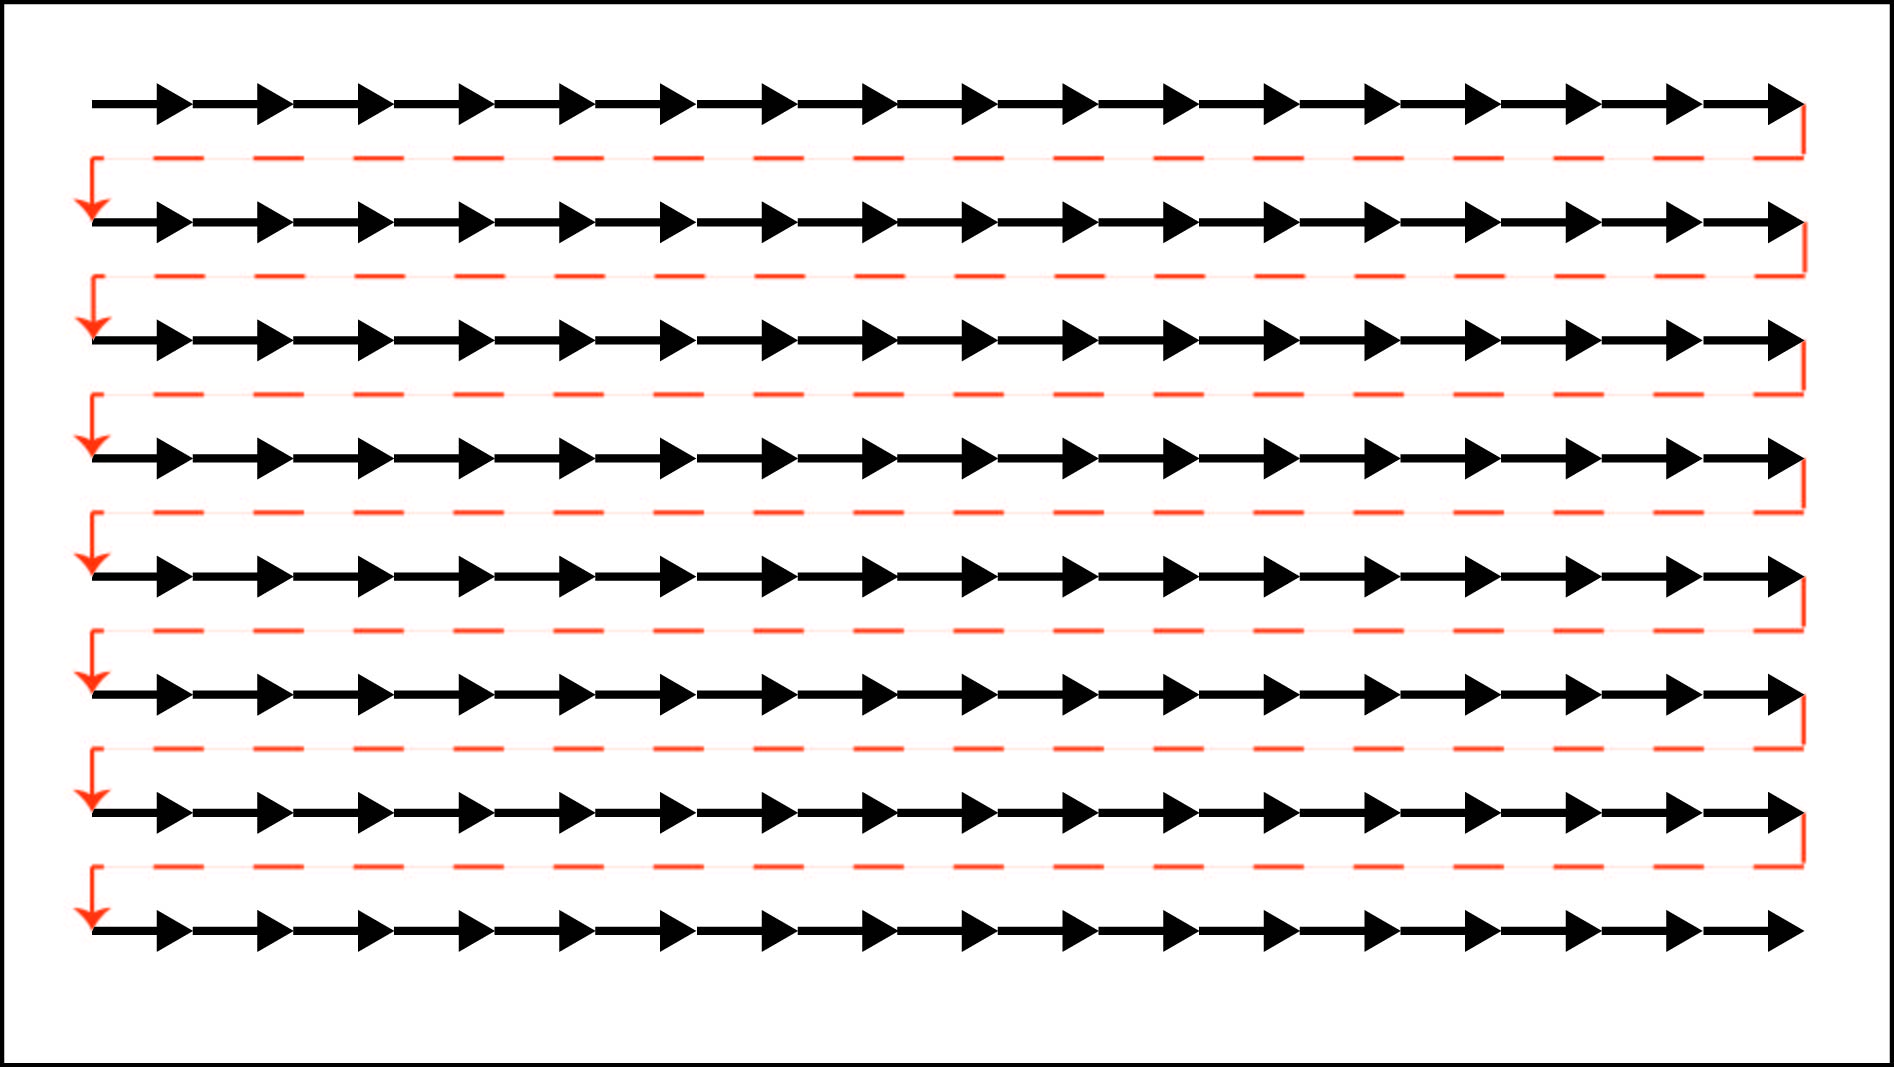
\includegraphics[width=12cm]{6_scanning.jpg}
	\caption{Proces skanowania - schemat przemieszczania okna detekcji na obrazie}
	\label{fig:scan_scheme}
\end{figure}
Skanowanie obrazu $1280\times 720$ wymaga wykonania $7\cdot16=112$ iteracji algorytmu dla kolejnych nieparzystych klatek, co trwa nieco mniej niż 4 sekundy. %TODO rozdzielczość tradycyjnie podaje się 1280 x 720, styl. przejście %ODP tak, ale to się nijak ma do tego, że jeśli traktować to jako tablicę pikseli to najpierw jednak podaje się wiersze, potem kolumny.
Proces ten może trwać krócej, jeśli w jego trakcie osiągnie się bardzo dobry wynik klasyfikacji, poniżej zadanego poziomu \textit{SVM\_strong\_threshold}=$-1$; w standardowej procedurze wystarczy zapamiętany najlepszy wynik poniżej \textit{SVM\_threshold}=$-0.1$. %TODO styl. kontroler natrafi %ODP OK

\subsubsection{Weryfikacja pierwszej detekcji}
Kolejny etap, weryfikacyjny, jest uruchamiany bezpośrednio po zakończeniu skanowania i polega na przeprowadzeniu 3 kolejnych iteracji SVM -- w trybie śledzenia (czyli na ograniczonym oknie, analizując obszar dla ostatniego wyniku SVM). %TODO podać/podkreślić, że już w ograniczonym oknie to się odbywa %ODP OK
Warunkiem przejścia przez ten etap jest, by wynik każdej iteracji był mniejszy od założonego maksimum \textit{SVM\_threshold}. 
W przeciwnym wypadku część PL przechodzi w stan bezczynności, ustawiana jest odpowiednia wartość statusu \textit{PL\_to\_PS\_status}, w odpowiedzi na którą część PS wyśle sygnał \textit{PS\_to\_PL\_run\_alg} rozpoczynający ponownie etap skanowania. Mechanizm ten stworzono, by kwestie decyzyjne związaną z dalszym postępowaniem przenieść do PS.

%TODO wprowadziłbym podział na podrozdziały.
%TODO a to czy to się powiodło/czy nie jest jakoś sygnalizowane ? %ODP Opisano wyżej
\subsubsection{Śledzenie}
Standardowe śledzenie opiera się na zweryfikowaniu wyniku ostatniej iteracji HOG+SVM, jednak proces uwzględnia jeszcze kilka elementów:
\begin{itemize}
	\item start algorytmu MeanShift -- wcześniej niedostępny algorytm MS ma możliwość rozpoczęcia pracy po zarejestrowaniu poprawnego wyniku klasyfikacji SVM (wartość mniejsza niż \textit{SVM\_strong\_threshold}). %TODO dobrego -> poprawnego %ODP OK
	Wzorcem dla MS zostanie obszar z kolejnej klatki obrazu -- kwadrat o środku w $\{x,y-30\}$ -- gdzie $\{x,y\}$ to aktualny środek obszaru wyliczonego przez algorytm SVM. 
	Podane przesunięcie w pionie pozwala rozpocząć śledzenie MS na obszarze w obrębie klatki piersiowej, wartość dobrano empirycznie.
	
	\item wyłączenie algorytmu MeanShift -- MS może przesunąć obszar śledzenia poza śledzony obiekt, na przykład w związku ze zmianą oświetlenia. %TODO słowo zbieżność chyba nie jest właściwe %ODP OK
	By się przed tym ustrzec, konieczne jest wyłączenie algorytmu, by w stosownym momencie ponownie go uruchomić. 
	Odpowiedni warunek sprawdza, czy punkt MeanShift nie jest zbyt oddalony od punktu zwracanego przez poprawnie działający algorytm SVM.
	
	\item utrata śledzonego obiektu -- jeśli wynik ostatniej klasyfikacji nie spełnia \textit{SVM\_threshold}, może to oznaczać potencjalną utratę śledzonej postaci z pola widzenia. 
	Wówczas położenie osoby jest określane przez wynik działania algorytmu MeanShift, który stanowić będzie również wejście dla kolejnych iteracji HOG+SVM (poprawione o wspomniane wyżej przesunięcie $30$). %TODO inicjatywa przejmowana (styl), offstet -> przesunięcie %ODP OK
	Warunkiem wyjścia z tego stanu (powrotu do standardowego śledzenia) jest osiągnięcie wyniku klasyfikacji rzędu \textit{SVM\_strong\_threshold}.
	Istotnym ograniczeniem jest wartość \textit{SVM\_lost\_iter}, która określa ilość iteracji, w których ten tryb może pracować -- domyślnie są to ok. 3 sekundy (100 iteracji), jednak użytkownik może tę wartość modyfikować poprzez zapis do rejestru 0xC z poziomu konsoli. %TODO jakie rejestry ??%ODP Opisano nieco wyżej w tabelach
	Skala w tym trybie nie jest aktualizowana -- zachowywana jest wartość z ostatnich poprawnych detekcji algorytmu HOG+SVM. %TODO to jest niejasne %ODP OK
\end{itemize} 

%TODO rozważyłbym też schamt tego

Celem śledzenia jest utrzymanie obiektu w środku kadru. Sprowadza się to do ustalenia określonych wartości zadanych:
\begin{itemize}
	\item położenie punktu środkowego SVM: $\{x_{set},y_{set}\}=\{640,450\}$ 
	\item odległość kamery od osoby: $4$m, co umożliwia pozytywną detekcję dla określonej skali obrazu: $z_{set}=3$ %TODO dlaczego tak %ODP Opisano niżej
\end{itemize}
Wartość $x_{set}$ jest dość oczywista i wyznacza dokładnie połowę szerokości kadru.
Wartość $y_{set}$ została dobrana eksperymentalnie i jest związana potrzebą utrzymania odpowiedniej wysokości przez drona -- ok $1.5$m (zależnie od skali).
Ostatecznie, dla skal użytych w projekcie: $2/2.5/3/3.5/4$, dobór $z_{set}=3$ jest najbardziej rozsądny ze względu szacowaną odległość postaci od drona -- $4$m -- oraz możliwość detekcji postaci w bliższej oraz dalszej odległości.

Uchyb regulacji jest wyznaczany po każdej iteracji algorytmu SVM. 
Opiera się na obliczeniu różnicy pomiędzy obecnymi koordynatami SVM, a ustalonymi wartościami zadanymi. %TODO jak wartością zadaną ? trzeba podać, że celem jest aby obiekt był w środku kadru %ODP uwzględniono to w tekście, ale jednak mamy do czynienia z wartościami zadanymi, od których odejmujemy aktualne wyniki - inaczej bym tego nie nazwał.
Ponadto, w przypadku skali zdecydowano, by obliczana była średnia krocząca 4 ostatnich wyników poprzez ich zsumowanie, a następnie przesunięcie bitowe o 2 w prawo, równe dzieleniu przez 4.
Taki zestaw danych jest co określoną liczbę iteracji (domyślnie 15, czyli $0.5$s) przepisywany do rejestru 0x04 do którego dostęp ma część PS. Flaga \textit{PL\_to\_PS\_control} ustawiana wówczas w sygnale GPIO wywołuje obsługę przerwania, skutkującego ruchem drona. Częstotliwość wysyłania takiego sygnału można konfigurować rejestrem \textit{SVM\_iter\_between\_control}.
%TODO jak ta komunikacja jest realizowana. %ODP OK

%TODO lepiej opisać ten temat, szczególnie te skala, bo to jest niejasne %ODP OK

\subsection{Komunikacja FPGA<->autopilot} %TODO Zynq

Wymiana informacji pomiędzy autopilotem a układem SoC bazuje na transmisji UART o standardowej prędkości równej 115200 bodów. 
Za transmisję po stronie układu SoC jest odpowiedzialna część PS, jednak istnieje możliwość lokalizacji sygnałów RxD oraz TxD po stronie części PL (wybór spośród większej liczby pinów) \cite{PYNQ_sch}. 
Z kolei na autopilocie skonfigurowano port TELEM 2 \cite{PixhawkSerial}. Warstwą transportową jest protokół MAVLink, który opisano w dodatku \ref{subsec:MAVLink}

Został on zaprojektowany w postaci plików nagłówkowych -- taka forma umożliwia łatwe wykorzystanie w aplikacji tworzonej na jeden z rdzeni procesora ARM dostępnego na SoC Zynq. %TODO raczej na jeden z rdzeni. %ODP OK
Ponadto, każda z dostępnych wiadomości ma swój podzbiór funkcji umożliwiających proste pakowanie w zestaw bajtów lub poprawne sparsowanie odebranych informacji.

%TODO To by się przydało opisać w jakimś dodatku, a tu podać ref %ODP OK


\subsubsection{Aplikacja uruchomiona na procesorze ARM układu SoC Zynq}

O ile część PL układu Zynq jest tworzona w środowisku Xilinx Vivado, to narzędziem deweloperskim obsługującym PS jest inny program będący częścią pakietu firmy Xilinx -- SDK (Software Development Kit). %TODO styl. suity !!! -> pakietu %ODP OK
By jednak możliwe było rozpoczęcie pracy, konieczne jest zaimportowanie z Vivado tzw. konfiguracji sprzętowej, czyli informacji o dostępnych w PS peryferiach, oraz połączeniach pomiędzy PS a PL.

Jednym z nich jest GPIO, do którego podłączony został sygnał \textit{trigger\char`_algorithm}, status algorytmów oraz wartości uchybu regulacji. %TODO "wystawienie" %ODP OK
Odpowiednio skonfigurowane GPIO może generować przerwania, co wykorzystano jako reakcję na zmianę stanu któregokolwiek z opisanych wyżej sygnałów.

Pozostałymi peryferiami są dwa interfejsy UART. 
Lokalizacją dla pierwszego interfejsu UART są dwa piny, które połączono z odpowiednim portem autopilota. 
Aplikacja, korzystając z biblioteki MAVLink, jest w stanie zdekodować i sparsować ramki przychodzące oraz odpowiednio spakować komendy wysyłane do autopilota.

Drugi interfejs UART, wyprowadzony domyślnie na wyjście microUSB płyty PYNQ, stanowi połączenie z komputerem jako element różnorakich testów i debugowania w trakcie implementacji. 
Utworzono dla niego prostą formę terminala, który w odpowiedzi na komendy wpisywane z klawiatury komputera umożliwia zapis i odczyt z rejestrów testowych, wysyłanie określonych wiadomości do autopilota, ale przede wszystkim wyświetla odpowiednio sparsowane informacje wysyłane przez autopilot.

W aplikacji zaimplementowano nadrzędną maszynę stanu, której częstotliwość pracy jest nadana przez odbierane co sekundę wiadomości z autopilota o ID=0, które noszą nazwę „HEARTBEAT”. %TODO "tempo pracy" %ODP OK
Odpowiada ona za przygotowanie maszyny do śledzenia: uzbrojenie (komenda ARM), start (komenda TAKEOFF) i odczekanie określonego czasu przed rozpoczęciem skanowania. Wysłanie nowej komendy ruchu w trakcie etapu śledzenia jest realizowane niezależnie  podczas obsługi przerwania związanego z GPIO, po otrzymaniu sygnału \textit{PL\_to\_PS\_control}. Wykorzystywana jest w tym celu komenda SET\_POSITION\_TARGET\_LOCAL\_NED, której opis znajduje się w dodatku \ref{commands}. Warto zaznaczyć, że o ile oprogramowanie autopilota ArduCopter wyróżnia 14 trybów lotu drona, to trybem, który realizuje komendy ruchu wysyłane protokołem MAVLink, jest tryb GUIDED. Zostało to szerzej opisane w dodatku \ref{flightmodes}.
%TODO to jest niejasne, bo nie ma opisu jak się tym dronem steruje... %ODP OK, opisano w dodatku

Podstawowym warunkiem pracy maszyny stanu jest obecność sygnału \textit{trigger\char`_algorithm}. 
Po jego zboczu narastającym następuje próba uzbrojenia drona; po zmianie stanu sygnału na niski (zmiana stanu przełącznika aparatury radiowej) procesor wyśle komendę rozpoczynającą proces lądowania. %TODO dlaczego lądowania. %ODP Bo założyłem, że jest to koniec misji.
Bardziej szczegółowy opis komunikacji z dronem przedstawia schemat \ref{fig:PL_FSM_sch}.
Ostatecznie, przesunięcia dla każdej osi są obliczane według wzorów:
\begin{equation}
\left.\begin{aligned}
x_{mov}&= \frac{\boldmath{z_{set}}-z_{new}}{x_w}\\
y_{mov}&= \frac{x_{new}-\boldmath{x_{set}}}{z_{new}\cdot y_w}\\
z_{mov}&= \frac{y_{new}-\boldmath{y_{set}}}{z_{new}\cdot z_w},\\
\end{aligned}\right.
\end{equation}
%TODO jakoś dla mnie te skale są niejasne. %ODP Opisano wyżej i tutaj
gdzie: $y_{new}$, $x_{new}$, $z_{new}$ to informacje pochodzące z algorytmów MS/HOG+SVM, a \textit{$x_w$, $y_w$, $z_w$} są empirycznie dobranymi współczynnikami dopasowującymi wartości do jednostek. Nie bez znaczenia jest także skojarzona z wynikiem detekcji skala obrazu -- dla mniejszych skal (obiekt dalej od kamery) potrzebny jest większy ruch drona. Warto zwrócić uwagę na zmianę osi układu współrzędnych drona:
\begin{itemize}
	\item \textit{x} -- oś pozioma odpowiadająca kierunkowi ruchu samolotu (aspekt głębokości na obrazie),
	\item \textit{y} -- oś pozioma prostopadła do osi \textit{x},
	\item \textit{z} -- oś pionowa, zwrócona w dół.
\end{itemize}

\begin{figure}[ht]
	\centering
	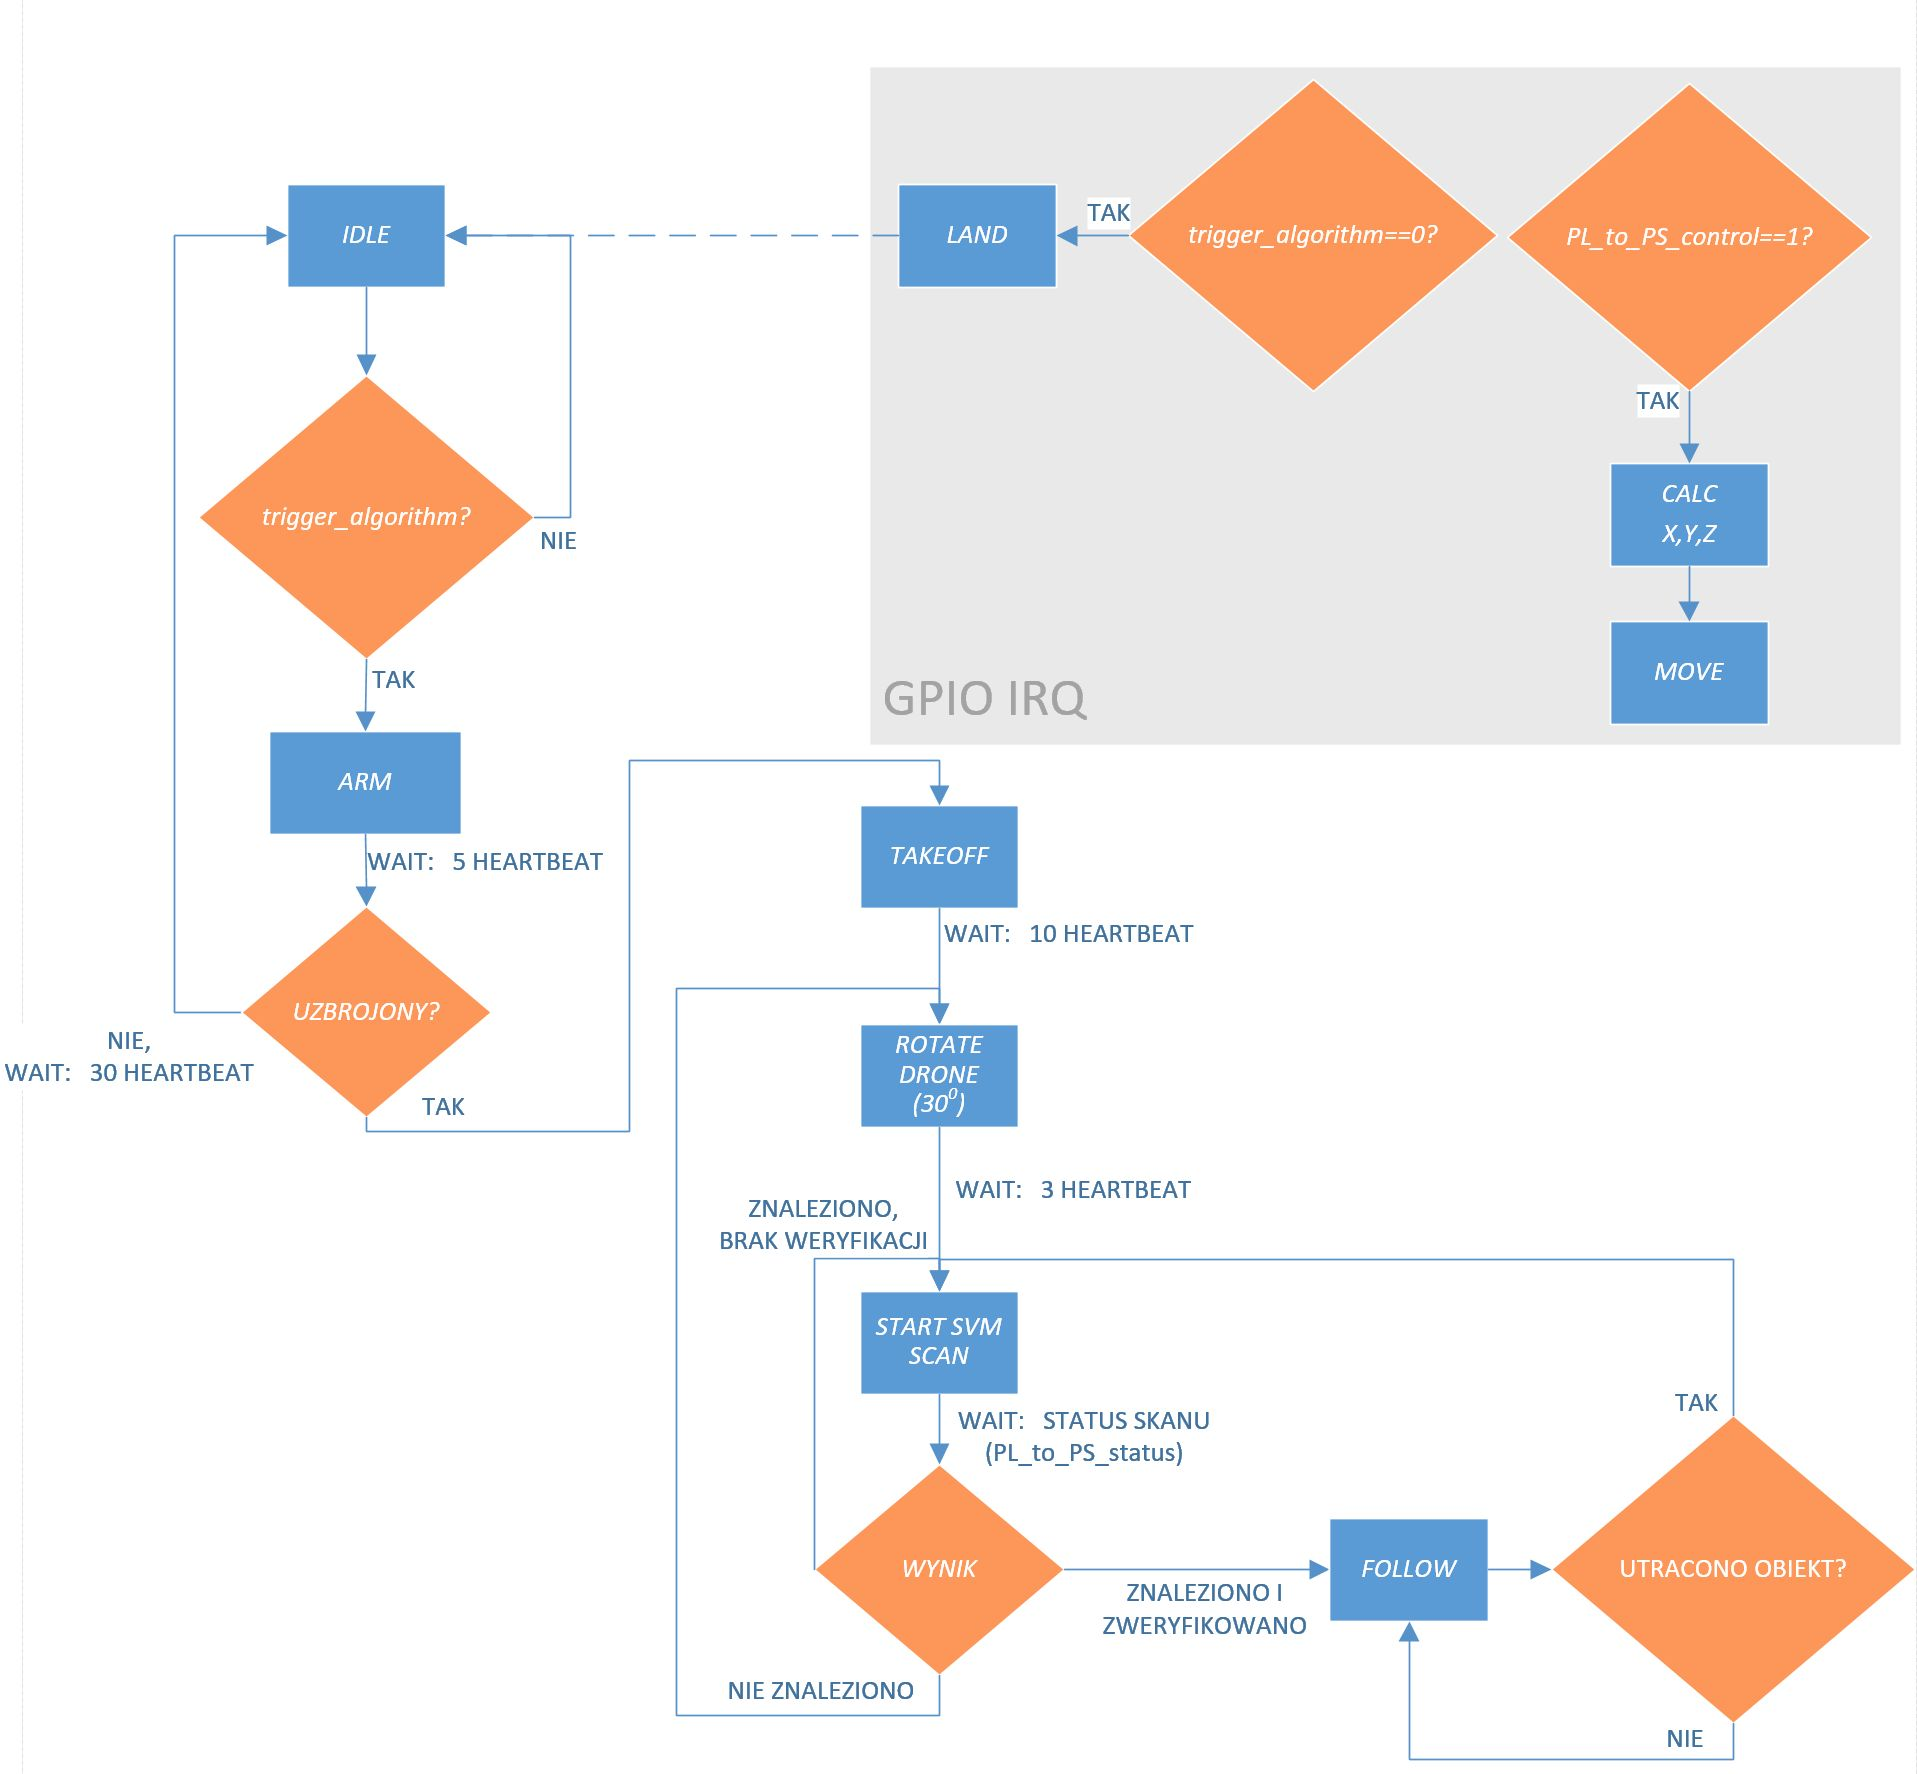
\includegraphics[width=16cm]{5_PS_FSM.jpg}
	\caption{Schemat działania aplikacji w PS}
	\label{fig:PL_FSM_sch}
\end{figure}
Domyślnie, maszyna stanu znajduje się w trybie bezczynności i oczekuje na pojawienie się sygnału \textit{trigger\char`_algorithm}. Wówczas podejmowana jest próba uzbrojenia z czasem oczekiwania 5 sekund. Autopilot wykonuje wtedy serię pomiarów weryfikacyjnych. Często ma jednak miejsce sytuacja, w której dron nie zostanie uzbrojony np. w wyniku niedokładnych pomiarów GPS. Jeśli proces ten się nie powiódł (informacja o stanie drona jest przesyłana z wiadomością HEARTBEAT), mija kolejne 30 sekund, i ponawiana jest próba uzbrojenia. W przeciwnym wypadku wysyłana jest komenda TAKEOFF z parametrem określającym docelową wysokość drona. Po kolejnych 10 sekundach dron potwierdza responsywność, obracając się o 30 stopni zgodnie z ruchem wskazówek zegara i po 3 sekundach rozpoczyna proces skanowania. PS jest informowane o stanie tego procesu poprzez sygnał \textit{PL\_to\_PS\_status} -- w oparciu o aktualizację jego wartości maszyna stanu wymusza obrót urządzenia i nowe skanowanie (brak detekcji,) powtórzenie skanowania dla obecnej orientacji (brak weryfikacji), lub przechodzi do trybu śledzenia. W maszynie stanu ten etap został on zrealizowany dość pasywnie, bowiem analizuje jedynie stan detekcji i w przypadku permanentnej utraty obiektu z pola widzenia następuje powrót do procedury skanowania. Za wydawanie komend ruchu odpowiada funkcja obsługi przerwania GPIO, która jest uruchamiana po każdej zmianie tego sygnału.
%TODO Brak omówienia schematu

%TODO a jakieś ograniczenia na ten ruch. min z max z maks zmiana ?

\section{Podsumowanie stworzonej architektury}

Ostatecznie architekturę programowo-sprzętową może przedstawić schemat \ref{fig:5_top_scheme}, opisujący najważniejsze zależności pomiędzy modułami. Zauważyć można podobieństwo sygnałów związanych z implementacją poszczególnych algorytmów - upraszcza to ich integrację w module TOP\_LAYER.

\begin{figure}[ht]
	\centering
	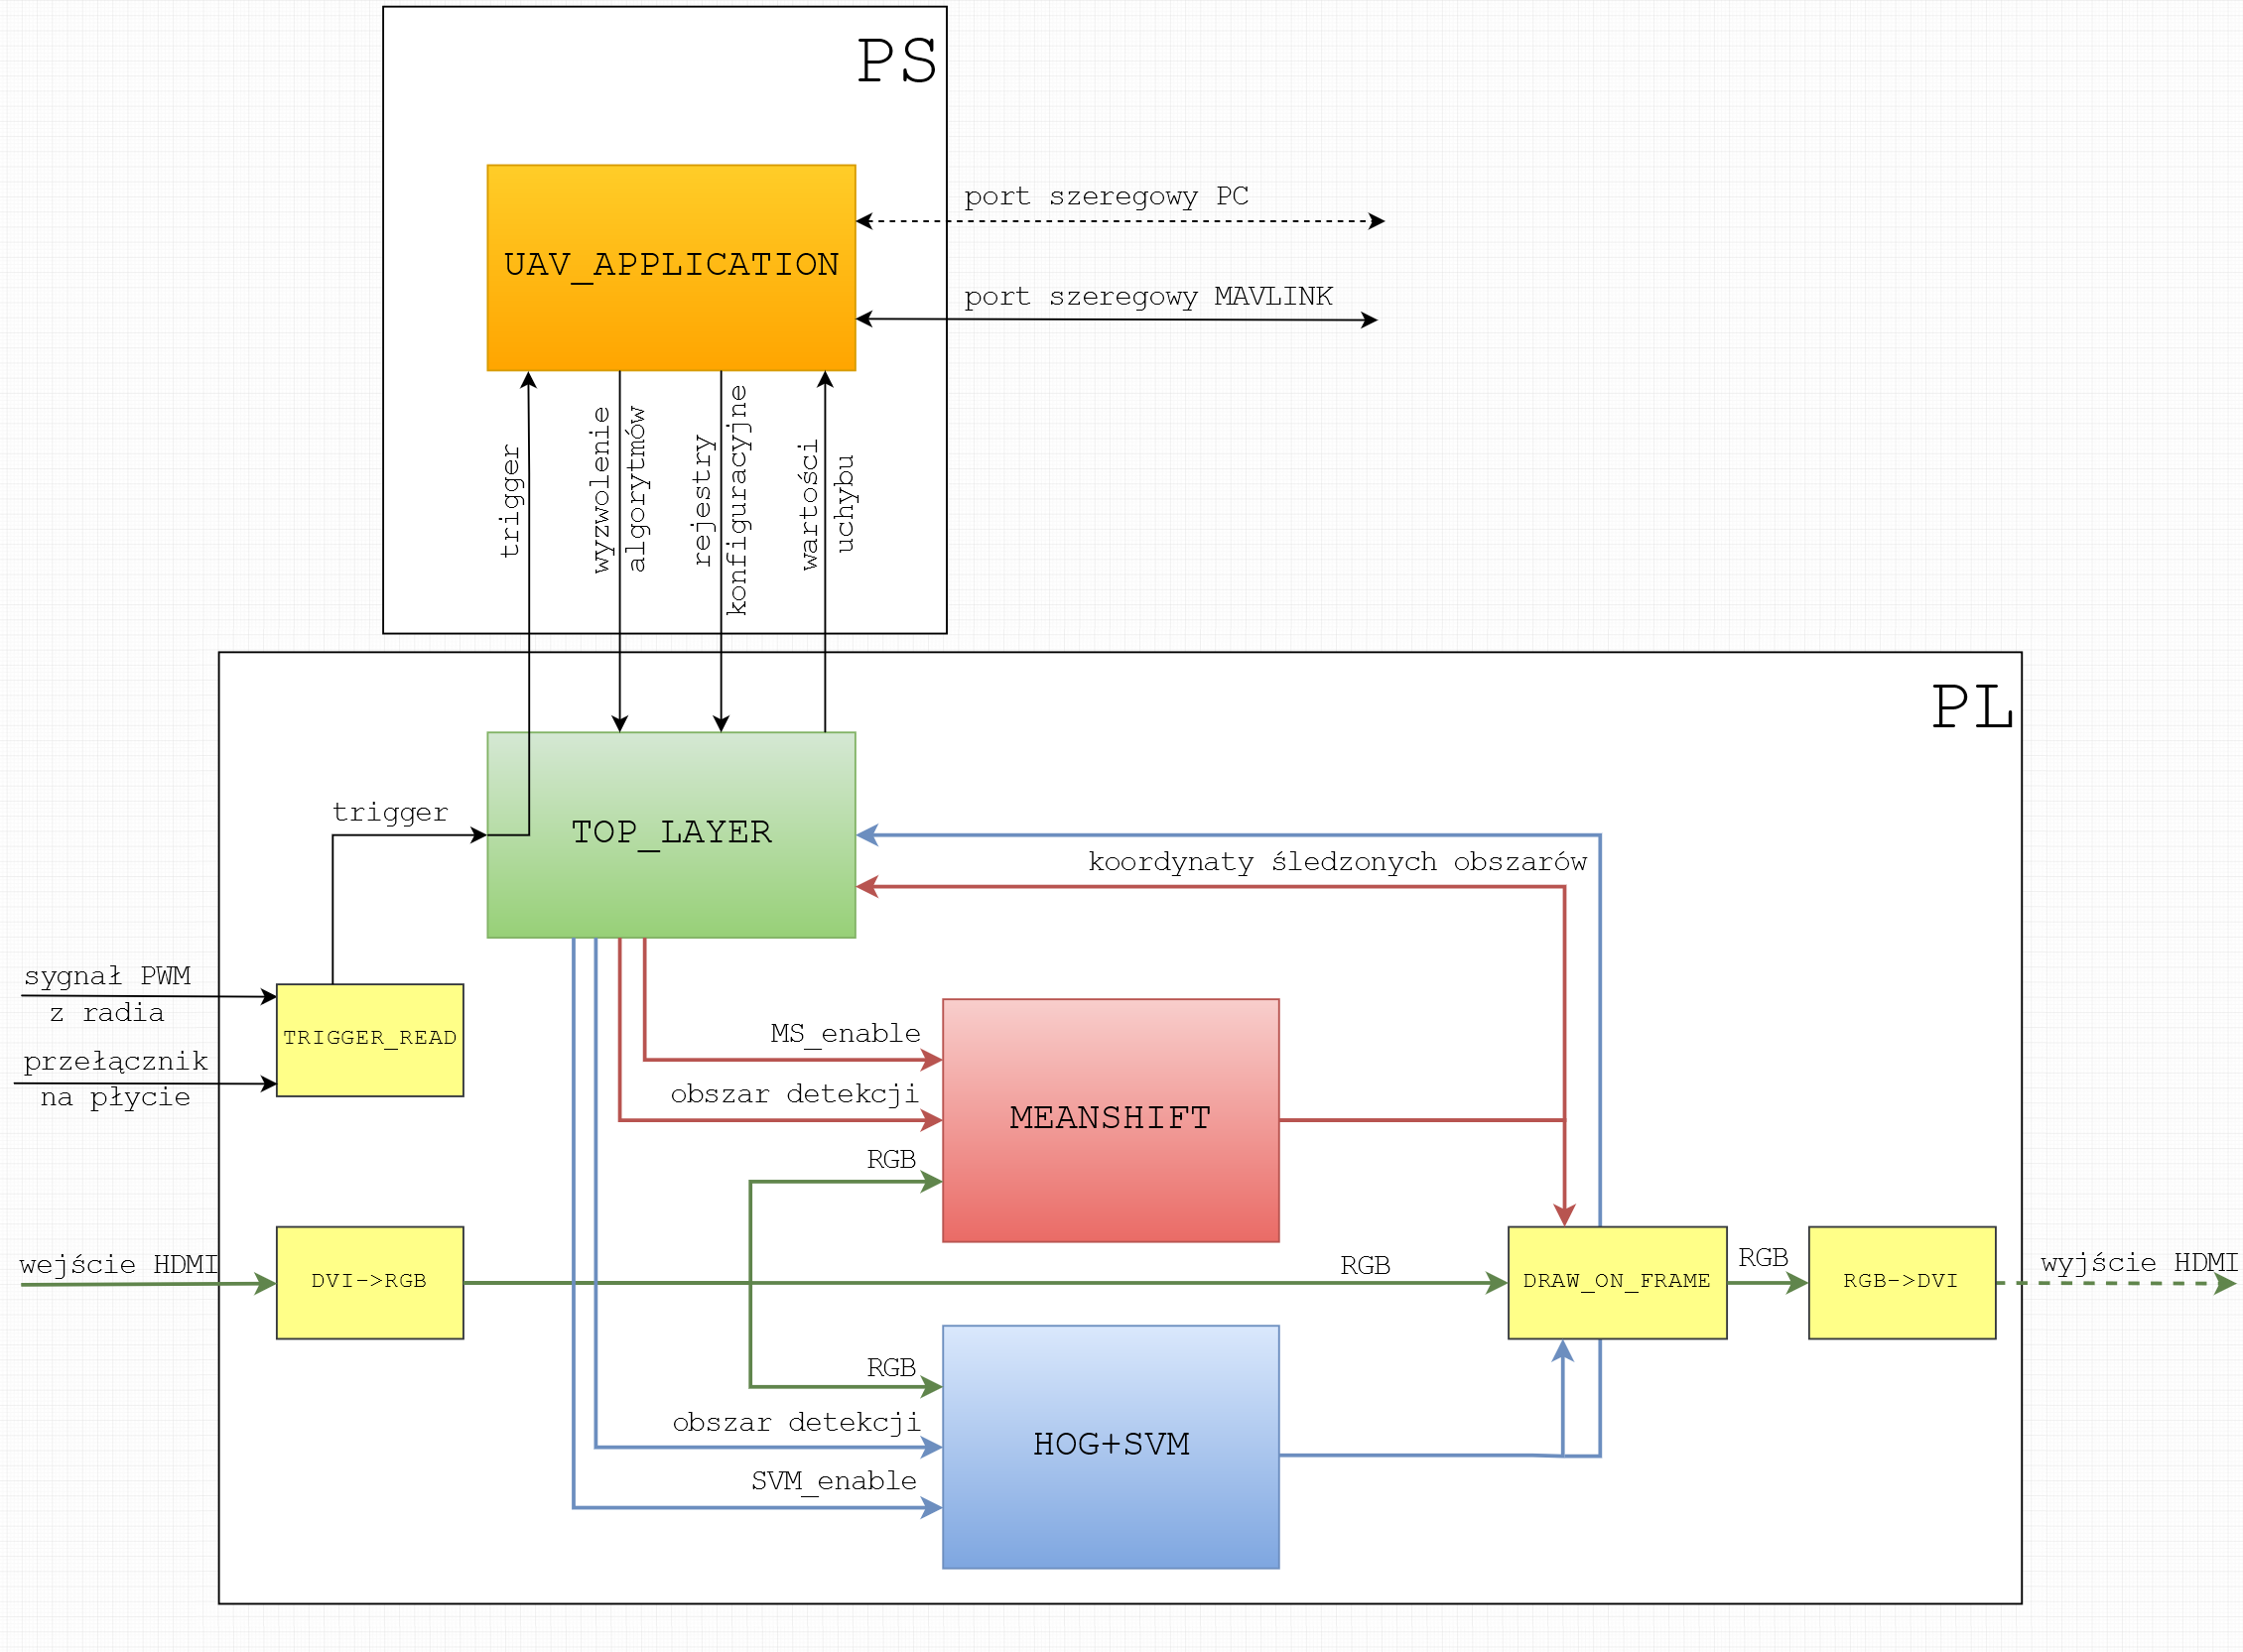
\includegraphics[width=16cm]{5_top_scheme.png}
	\caption{Schemat architektury programowo-sprzętowej}
	\label{fig:5_top_scheme}
\end{figure}

Proces implementacji sprzętowej szedł w parze z nadzorem wykorzystania zasobów w układzie. Nieodpowiednie zagospodarowanie dostępnymi w logice elementami mogłoby mieć wpływ na rozmieszczenie (routing) sygnałów i problemy związane z czasami ich ustalania lub podtrzymania (setup/hold time). Tabele \ref{tab:utilizationMS}, \ref{tab:utilizationHOG} oraz \ref{tab:utilizationOverall} przedstawiają wykorzystanie zasobów w układzie Zynq 7Z020.
\begin{table}[ht]
	\centering
	\caption{Wykorzystanie zasobów dla implementacji algorytmu MeanShift}
	\captionsetup{justification=centering,margin=1cm}
	\begin{tabular}{|P{3cm} |P{3cm} |P{3cm}|P{4cm}|}	
		\hline
		\rowcolor{lightgray} Rodzaj zasobu & Wykorzystane & Dostępne & Wykorzystanie [\%]\\ 
		LUT		& 5255	& 53200 & 9.8\\ 
		\hline
		FF		& 8562	& 106400 & 8.0\\ 
		\hline
		BRAM	& 25.5	& 140 & 18.2\\ 
		\hline
		DSP		& 28	& 220 & 12.7\\ 
		\hline		
	\end{tabular}

	\label{tab:utilizationMS}
\end{table}

\begin{table}[ht]
	\centering
	\caption{Wykorzystanie zasobów dla implementacji algorytmu HOG+SVM}
	\captionsetup{justification=centering,margin=1cm}
	\begin{tabular}{|P{3cm} |P{3cm} |P{3cm}|P{4cm}|}	
		\hline
		\rowcolor{lightgray} Rodzaj zasobu & Wykorzystane & Dostępne & Wykorzystanie [\%]\\ 
		LUT		& 23894	& 53200 & 44.9\\ 
		\hline
		FF		& 32668	& 106400 & 30.7\\ 
		\hline
		BRAM	& 66	& 140 & 47.1\\ 
		\hline
		DSP		& 55	& 220 & 25\\ 
		\hline		
	\end{tabular}
	\label{tab:utilizationHOG}
\end{table}

\begin{table}[ht]
	\centering
	\caption{Wykorzystanie zasobów - pełna architektura}	
	\captionsetup{justification=centering,margin=1cm}
	\begin{tabular}{|P{3cm} |P{3cm} |P{3cm}|P{4cm}|}	
		\hline
		\rowcolor{lightgray} Rodzaj zasobu & Wykorzystane & Dostępne & Wykorzystanie [\%]\\ 
		LUT		& 33729	& 53200 & 63.4\\ 
		\hline
		FF		& 46385	& 106400 & 43.6\\ 
		\hline
		BRAM	& 92	& 140 & 65.7\\ 
		\hline
		DSP		& 83	& 220 & 37.7\\ 
		\hline		
	\end{tabular}
	\label{tab:utilizationOverall}
\end{table} 

Dodatkowo, postanowiono dokonać estymacji poboru mocy przez układ. W tym celu w środowisku Vivado wygenerowano raport w oparciu o określenie temperatury otoczenia równej $25^{\circ}$C i wybór najbardziej pesymistycznego poziomu estymacji. Z dokumentu wynika, że całkowity pobór mocy w układzie nie powinien przekraczać $3.5$W, z czego jednak aż $1.3$W to wartość pobierana przez część PS. Fragment logiki realizujący metodę HOG+SVM potrzebuje $0.99$W, natomiast MeanShift zaledwie $0.11$W.